% Options for packages loaded elsewhere
\PassOptionsToPackage{unicode}{hyperref}
\PassOptionsToPackage{hyphens}{url}
\PassOptionsToPackage{dvipsnames,svgnames,x11names}{xcolor}
\documentclass[
  11pt,
  openany,
  oneside]{book}
\usepackage{xcolor}
\usepackage[margin=2.2cm,top=2.4cm,bottom=2.4cm]{geometry}
\usepackage{amsmath,amssymb}
\setcounter{secnumdepth}{-\maxdimen} % remove section numbering
\usepackage{iftex}
\ifPDFTeX
  \usepackage[T1]{fontenc}
  \usepackage[utf8]{inputenc}
  \usepackage{textcomp} % provide euro and other symbols
\else % if luatex or xetex
  \usepackage{unicode-math} % this also loads fontspec
  \defaultfontfeatures{Scale=MatchLowercase}
  \defaultfontfeatures[\rmfamily]{Ligatures=TeX,Scale=1}
\fi
\usepackage{lmodern}
\ifPDFTeX\else
  % xetex/luatex font selection
\fi
% Use upquote if available, for straight quotes in verbatim environments
\IfFileExists{upquote.sty}{\usepackage{upquote}}{}
\IfFileExists{microtype.sty}{% use microtype if available
  \usepackage[]{microtype}
  \UseMicrotypeSet[protrusion]{basicmath} % disable protrusion for tt fonts
}{}
\makeatletter
\@ifundefined{KOMAClassName}{% if non-KOMA class
  \IfFileExists{parskip.sty}{%
    \usepackage{parskip}
  }{% else
    \setlength{\parindent}{0pt}
    \setlength{\parskip}{6pt plus 2pt minus 1pt}}
}{% if KOMA class
  \KOMAoptions{parskip=half}}
\makeatother
\usepackage{listings}
\newcommand{\passthrough}[1]{#1}
\lstset{defaultdialect=[5.3]Lua}
\lstset{defaultdialect=[x86masm]Assembler}
\usepackage{longtable,booktabs,array}
\newcounter{none} % for unnumbered tables
\usepackage{calc} % for calculating minipage widths
% Correct order of tables after \paragraph or \subparagraph
\usepackage{etoolbox}
\makeatletter
\patchcmd\longtable{\par}{\if@noskipsec\mbox{}\fi\par}{}{}
\makeatother
% Allow footnotes in longtable head/foot
\IfFileExists{footnotehyper.sty}{\usepackage{footnotehyper}}{\usepackage{footnote}}
\makesavenoteenv{longtable}
\usepackage{graphicx}
\makeatletter
\newsavebox\pandoc@box
\newcommand*\pandocbounded[1]{% scales image to fit in text height/width
  \sbox\pandoc@box{#1}%
  \Gscale@div\@tempa{\textheight}{\dimexpr\ht\pandoc@box+\dp\pandoc@box\relax}%
  \Gscale@div\@tempb{\linewidth}{\wd\pandoc@box}%
  \ifdim\@tempb\p@<\@tempa\p@\let\@tempa\@tempb\fi% select the smaller of both
  \ifdim\@tempa\p@<\p@\scalebox{\@tempa}{\usebox\pandoc@box}%
  \else\usebox{\pandoc@box}%
  \fi%
}
% Set default figure placement to htbp
\def\fps@figure{htbp}
\makeatother
\setlength{\emergencystretch}{3em} % prevent overfull lines
\providecommand{\tightlist}{%
  \setlength{\itemsep}{0pt}\setlength{\parskip}{0pt}}
% =====================================================================
% House style for the samarjithbiswas.com handbook series.
% Matched to the "On-Device LLMs for Engineering Software" toolkit:
% IBM Plex Sans body, teal/slate palette, titlesec headings, fancyhdr,
% tcolorbox callouts, a dark code-listing style. Injected by pandoc as
% header-includes, so amsmath / graphicx / xcolor / hyperref / longtable
% are already loaded by the pandoc book template; we only add styling.
% =====================================================================
\usepackage[T1]{fontenc}
\usepackage{plex-sans}
\renewcommand{\familydefault}{\sfdefault}
\usepackage[scaled=0.90]{plex-mono}
\usepackage{microtype}
\usepackage{titlesec}
\usepackage{fancyhdr}
\usepackage{booktabs}
\usepackage{caption}
\usepackage{tcolorbox}
\tcbuselibrary{breakable, skins}

% --- Brand palette (teal series + a navy accent for the space title) ---
\definecolor{brandTeal}{HTML}{0d9488}
\definecolor{brandTealDk}{HTML}{0f766e}
\definecolor{brandPurple}{HTML}{7c3aed}
\definecolor{brandAmber}{HTML}{d97706}
\definecolor{brandSlate}{HTML}{0f172a}
\definecolor{brandGray}{HTML}{475569}
\definecolor{brandLight}{HTML}{f1f5f9}
\definecolor{spaceNavy}{HTML}{16243a}
\definecolor{codeBg}{HTML}{0f172a}
\definecolor{codeFg}{HTML}{e2e8f0}
\definecolor{calloutBlue}{HTML}{dbeafe}
\definecolor{calloutAmber}{HTML}{fef3c7}
\definecolor{calloutGreen}{HTML}{dcfce7}

% --- Manual chapter/section numbers live in the headings (e.g. "3A.",
% "4.1"); suppress LaTeX's automatic numbering so nothing is doubled.
% Parts stay numbered (Part I .. Part VII). ---
\setcounter{secnumdepth}{-1}
\setcounter{tocdepth}{1}

% --- Hyperlink colours. pandoc injects this header BEFORE it loads hyperref,
% so \hypersetup is not yet defined here; defer it to \AtBeginDocument, which
% runs after hyperref is loaded. (Calling it inline printed the options as body
% text on page 1.) ---
\AtBeginDocument{%
  \hypersetup{colorlinks=true, linkcolor=brandTealDk, citecolor=brandTealDk,
              urlcolor=brandTeal, linktoc=all,
              pdftitle={Space-Based Data Center Infrastructure: A Multi-Physics Approach},
              pdfauthor={Samarjith Biswas, PhD}}%
}

% --- Headings (centered, monograph-style chapter openers) ---
\titleformat{\chapter}[display]
  {\sffamily\filcenter}
  {\large\bfseries\color{brandTeal}\MakeUppercase{\chaptertitlename}}
  {10pt}
  {\fontsize{25}{30}\selectfont\bfseries\color{brandSlate}}
  [\vskip12pt{\color{brandTeal}\titlerule[1.2pt]}]
\titlespacing*{\chapter}{0pt}{24pt}{34pt}
\titleformat{\section}
  {\Large\bfseries\color{brandTealDk}}{}{0em}{}
\titleformat{\subsection}
  {\large\bfseries\color{brandSlate}}{}{0em}{}
\titleformat{\subsubsection}
  {\normalsize\bfseries\color{brandGray}}{}{0em}{}
\titlespacing*{\chapter}{0pt}{12pt}{30pt}
\titlespacing*{\section}{0pt}{16pt}{6pt}
\titlespacing*{\subsection}{0pt}{12pt}{4pt}

% --- Part pages ---
\titleformat{\part}[display]
  {\sffamily\centering}
  {\Large\bfseries\color{brandTeal}\MakeUppercase{\partname~\thepart}}
  {10pt}
  {\Huge\bfseries\color{brandSlate}}

% --- Running header / footer (chapter title runs in the header) ---
\renewcommand{\chaptermark}[1]{\markboth{#1}{}}
\pagestyle{fancy}
\fancyhf{}
\fancyhead[L]{\small\itshape\color{brandGray}\nouppercase{\leftmark}}
\fancyhead[R]{\small\color{brandGray}\thepage}
\fancyfoot[C]{\small\color{brandGray}Space-Based Data Center Infrastructure \textbullet{} Samarjith Biswas \textbullet{} 2026}
\renewcommand{\headrulewidth}{0.4pt}
\renewcommand{\headrule}{{\color{brandTeal}\hrule height 1pt}}
\renewcommand{\footrulewidth}{0pt}
% Plain style (chapter opening pages) keeps the footer, drops the header rule
\fancypagestyle{plain}{\fancyhf{}\fancyfoot[C]{\small\color{brandGray}Space-Based Data Center Infrastructure \textbullet{} Samarjith Biswas \textbullet{} 2026}\renewcommand{\headrulewidth}{0pt}\renewcommand{\footrulewidth}{0pt}}

% --- Code listings (pandoc passes fenced code through listings) ---
\lstset{
  basicstyle=\ttfamily\footnotesize\color{codeFg},
  backgroundcolor=\color{codeBg},
  keywordstyle=\color{brandTeal!80!white}\bfseries,
  stringstyle=\color{brandAmber!85!white},
  commentstyle=\color{brandGray!85!white}\itshape,
  numberstyle=\tiny\color{brandGray}, numbers=left, numbersep=8pt,
  showstringspaces=false, breaklines=true, breakatwhitespace=true,
  frame=none, framesep=8pt, xleftmargin=12pt, xrightmargin=8pt,
  aboveskip=10pt, belowskip=10pt,
  morekeywords={def,return,import,from,as,for,while,if,elif,else,class,with,lambda,True,False,None,and,or,not,in,np,self},
}

% --- Callout boxes (available for future hand-authored notes) ---
\newtcolorbox{insightbox}[1][]{colback=calloutBlue, colframe=blue!50!brandSlate,
  boxrule=0pt, leftrule=4pt, arc=2pt, fonttitle=\bfseries, title={Key insight},
  coltitle=blue!60!brandSlate, top=8pt, bottom=8pt, breakable, #1}
\newtcolorbox{tipbox}[1][]{colback=calloutGreen, colframe=brandTeal,
  boxrule=0pt, leftrule=4pt, arc=2pt, fonttitle=\bfseries, title={Result},
  coltitle=brandTealDk, top=8pt, bottom=8pt, breakable, #1}
\newtcolorbox{warnbox}[1][]{colback=calloutAmber, colframe=brandAmber,
  boxrule=0pt, leftrule=4pt, arc=2pt, fonttitle=\bfseries, title={Caveat},
  coltitle=brandAmber, top=8pt, bottom=8pt, breakable, #1}

% --- Figures sit centred and never overflow the text block ---
\setkeys{Gin}{width=0.86\linewidth, keepaspectratio}
\captionsetup{font=small, labelfont={bf,color=brandTealDk}}
\usepackage{bookmark}
\IfFileExists{xurl.sty}{\usepackage{xurl}}{} % add URL line breaks if available
\urlstyle{same}
\hypersetup{
  colorlinks=true,
  linkcolor={brandTealDk},
  filecolor={Maroon},
  citecolor={Blue},
  urlcolor={Blue},
  pdfcreator={LaTeX via pandoc}}

\author{}
\date{}

\begin{document}
\frontmatter

% ---------------------------------------------------------------------
% Complete front matter, monograph style. Injected by pandoc as
% include-before-body, so it runs after \frontmatter and before \mainmatter.
% Order: half-title, title page (navy panel matching the website book card),
% colophon/copyright, dedication, table of contents, list of figures, list
% of tables, preface, acknowledgments. The contents/lists are emitted here
% (pandoc's own --toc is disabled in build_book.py) so the ordering is exact.
% Uses \clearpage only (never \cleardoublepage) so the one-sided layout adds
% no blank pages.
% ---------------------------------------------------------------------

% ---------- Full-bleed designed cover ----------
\thispagestyle{empty}%
\newgeometry{margin=0pt}%
\noindent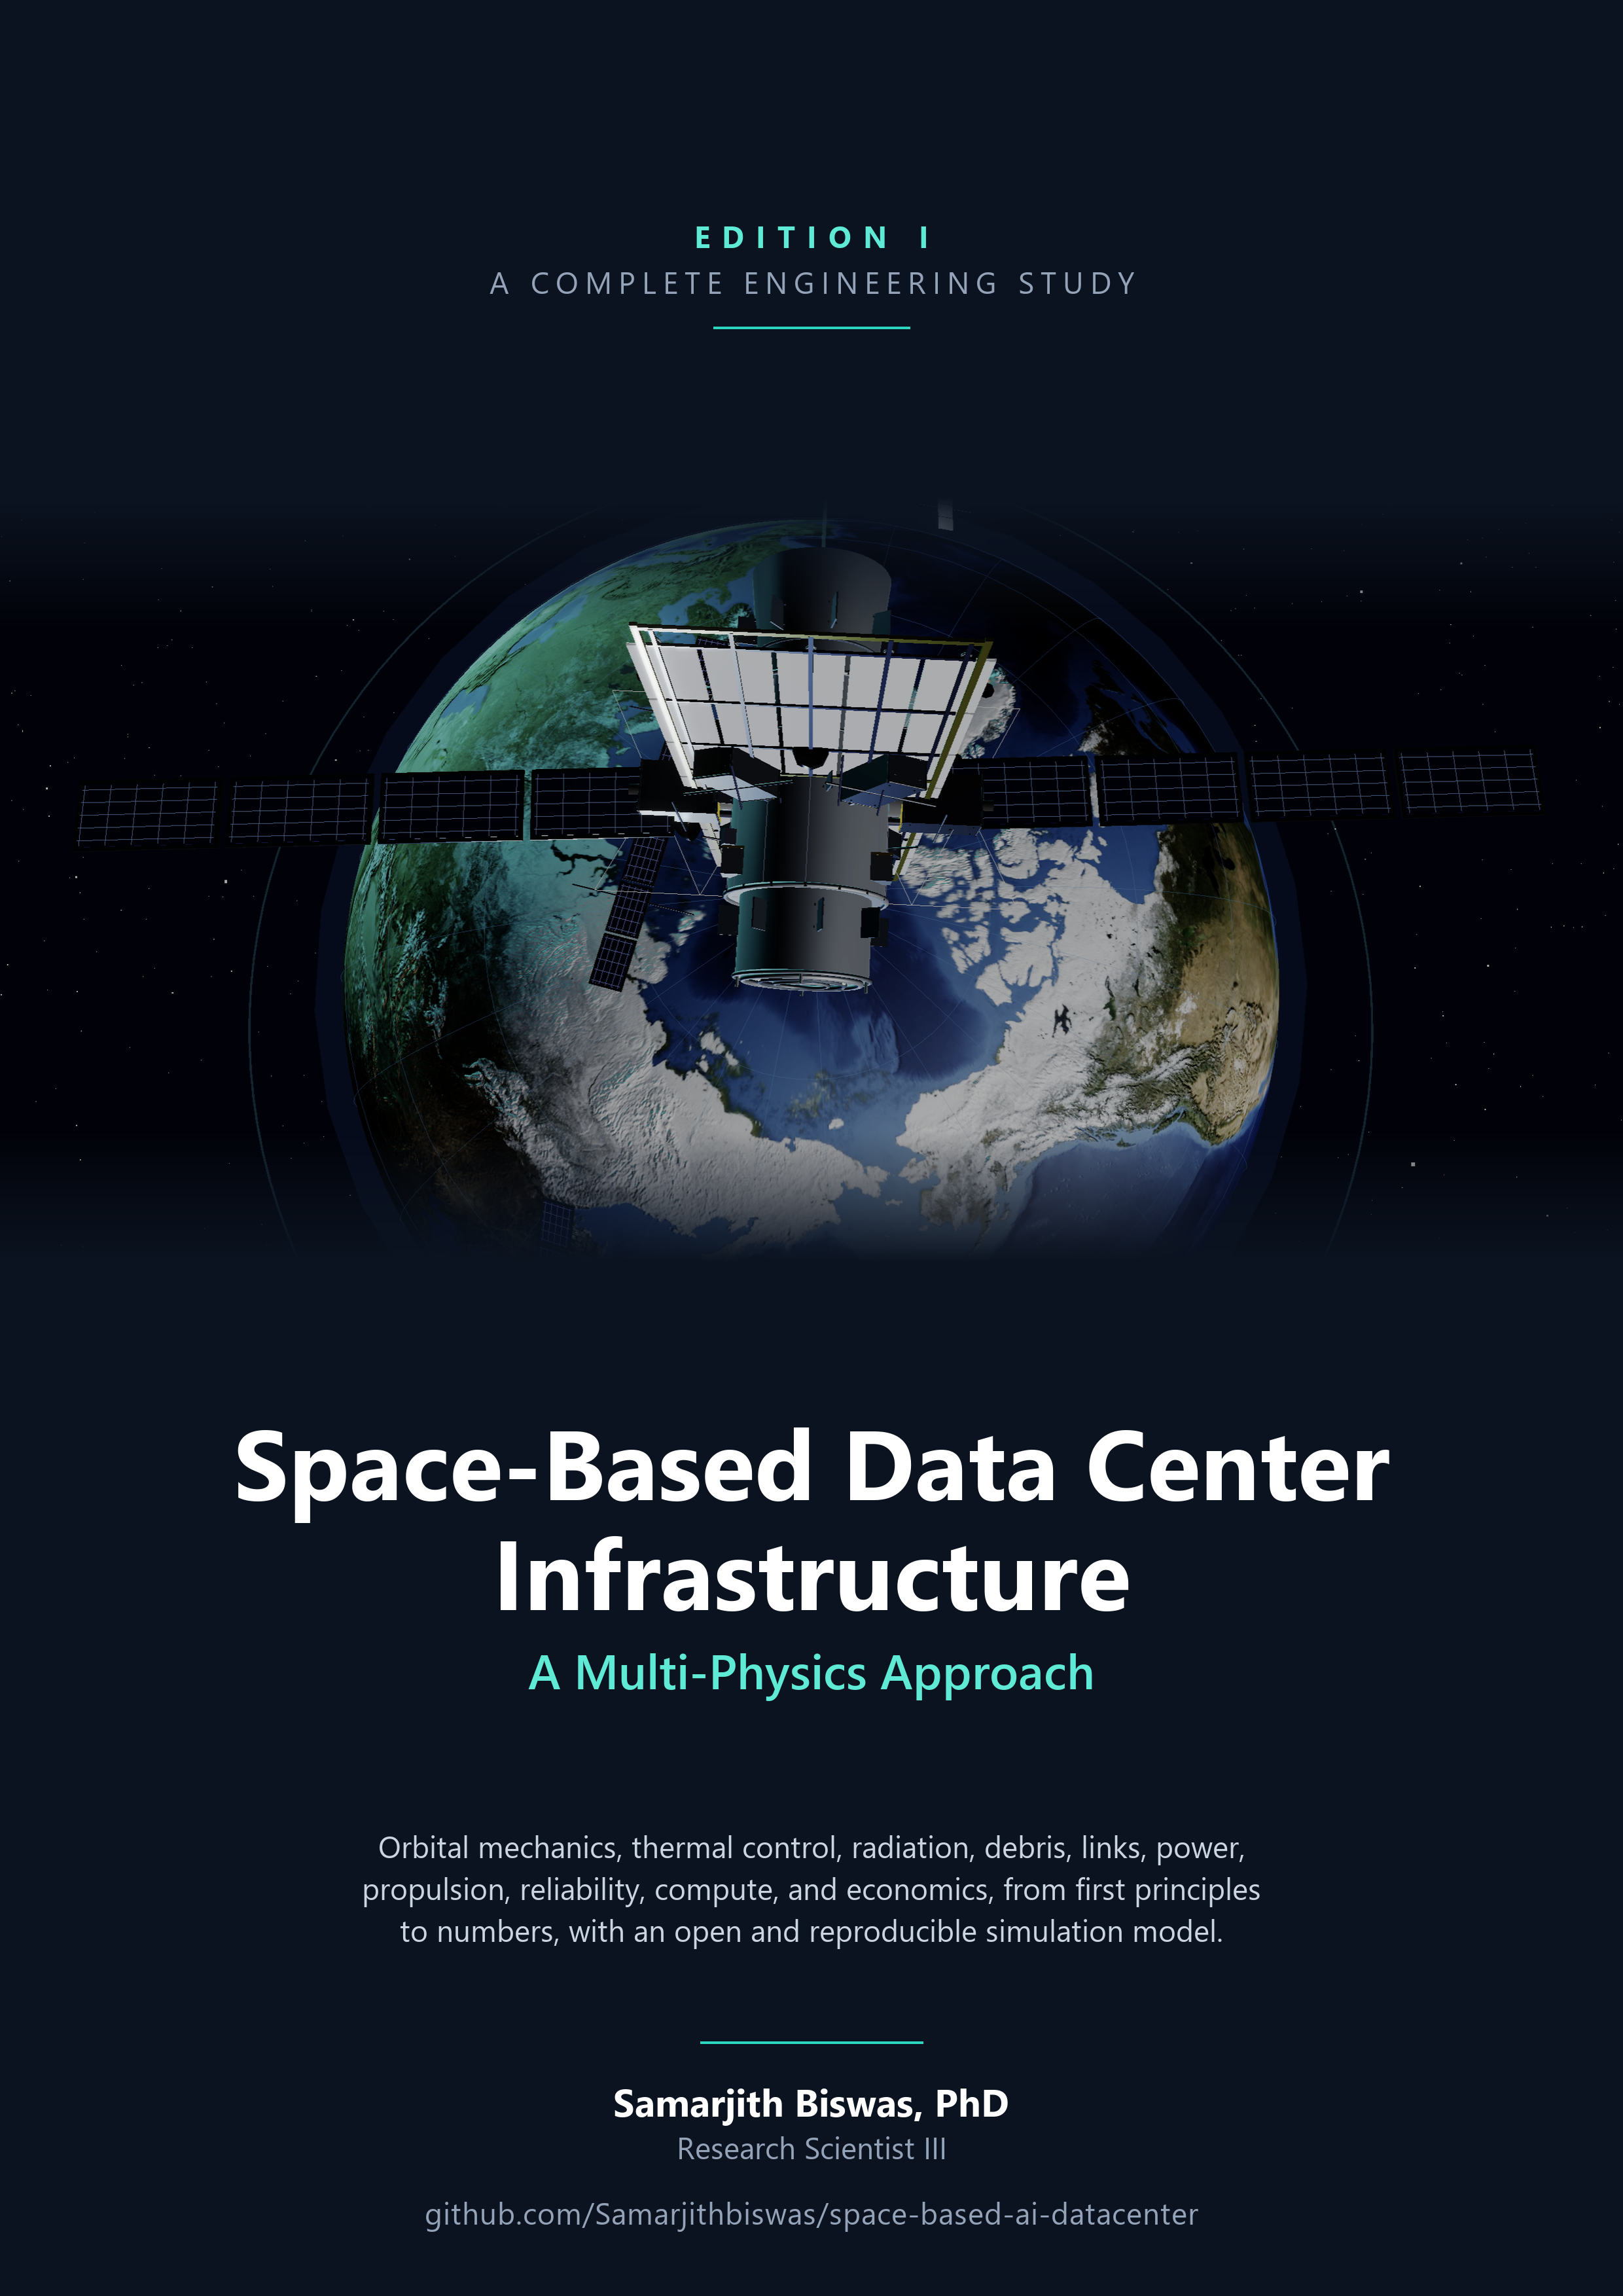
\includegraphics[width=\paperwidth,height=\paperheight,keepaspectratio=false]{cover_art.png}%
\restoregeometry
\clearpage

% ---------- Colophon / copyright ----------
\thispagestyle{empty}
\vspace*{\fill}
\noindent{\sffamily\small\color{brandGray}%
\textbf{\color{brandSlate}Space-Based Data Center Infrastructure: A Multi-Physics Approach.}\\[2pt]
Edition I, 2026. By Samarjith Biswas, PhD.\\[10pt]
This work is released open access. The accompanying source code is licensed under the MIT License;
the text, figures, and equations are licensed under Creative Commons Attribution 4.0 (CC-BY 4.0).
You are free to read, share, cite, and adapt the work with attribution.\\[10pt]
Source repository (models, derivations, simulations, figures):\\
\texttt{github.com/Samarjithbiswas/space-based-ai-datacenter}\\[6pt]
Reference architecture: Google Project Suncatcher, arXiv:2511.19468.\\[10pt]
Every figure and every load-bearing number in this book is regenerated by the open repository.
Forward-looking quantities, including the launch-cost trajectory of Chapter 22, are presented as
projections with explicit uncertainty bands, not as guarantees. Independent reproduction and
correction are welcome.\\[10pt]
Typeset in IBM Plex Sans and IBM Plex Mono with pdf\LaTeX.\\[2pt]
Part of the samarjithbiswas.com research portfolio.
}
\clearpage

% ---------- Dedication ----------
\thispagestyle{empty}
\vspace*{0.32\textheight}
\begin{center}
{\itshape\large\color{brandGray} For the engineers who will actually have to fly this,\\[4pt]
and bring every satellite safely home.}
\end{center}
\clearpage

% ---------- Table of contents, list of figures, list of tables ----------
{\hypersetup{linkcolor=brandSlate}
\tableofcontents}
\clearpage
\listoffigures
\clearpage
\listoftables
\clearpage

% ---------- Preface ----------
\chapter*{Preface}
\addcontentsline{toc}{chapter}{Preface}
The energy and thermal demands of artificial-intelligence computing have outrun the pace at which
terrestrial infrastructure can be built. Clusters are now provisioned in tens to hundreds of megawatts,
and power, water, land, and grid interconnection have become the binding constraints rather than the
silicon. It is against that pressure that a once-fanciful idea, operating data centers in orbit, has
moved from the conference slide into the engineering review. Within a single recent year a
data-center-class accelerator was switched on in orbit, a second company placed compute hardware in low
Earth orbit, and a major laboratory published a reference design for a constellation of machine-learning
accelerators flying in tight formation. The question is no longer whether someone will try, but whether
the physics and the economics actually close.

This book is an attempt to answer that question the way an engineer would, from first principles and
without a thesis to sell. It builds the complete subsystem model of an orbital artificial-intelligence
data center, orbital mechanics, the space environment, thermal control, radiation, debris,
communications, power, attitude, propulsion, reliability, compute, integration, and economics, and for
each subsystem it derives the governing relations, reduces them to numbers, and checks those numbers
against an open simulation. A strict line is kept throughout between what has been demonstrated in flight
and what remains a projection. Where the analysis corrects an earlier assumption or contradicts a widely
repeated claim, it says so plainly; where a quantity is a vendor forecast rather than a measured result,
it is flagged as such and given an uncertainty band rather than a single confident figure.

The book is meant to be read by graduate engineers and mission designers, by researchers entering the
field, and by the teams actually building the early demonstrators. It is organized in parts that move
from context and environment through the spacecraft subsystems to integration, economics, and synthesis,
so that a reader can follow a single thread from a physical principle to a defensible number, or can
enter at the subsystem of interest. Every figure and every load-bearing value is regenerated by the
accompanying open-source model, which is released under a permissive licence and validated by an
automated test suite. Independent reproduction, and correction, are not only welcome but are the point of
putting the whole apparatus in the open.

\vspace{10pt}
\noindent{\itshape Samarjith Biswas}\\
{\small\color{brandGray} 2026}
\clearpage

% ---------- Acknowledgments ----------
\chapter*{Acknowledgments}
\addcontentsline{toc}{chapter}{Acknowledgments}
This work rests on the open scientific-computing ecosystem, NumPy, SciPy, and Matplotlib above all, and
on the public environmental models and datasets maintained by the world's space agencies, including the
NRLMSIS atmosphere model, NASA ORDEM and the ESA MASTER and DRAMA debris tools, the SHIELDOSE and
AE/AP radiation models, and the public regulatory record of the United States Federal Communications
Commission. It also owes a debt to the authors of the reference architecture, whose decision to put
concrete numbers into the open made independent scrutiny possible in the first place. Finally, the shape
of this book was improved by readers of the earlier report who pressed, rightly, for reproducibility and
for an honest treatment of survivability rather than thermal feasibility alone.
\clearpage

\mainmatter
\section{An engineering analysis of a space-based AI compute
constellation}\label{an-engineering-analysis-of-a-space-based-ai-compute-constellation}

\textbf{Author:} Samarjith Biswas, PhD \textbf{Date:} June 2026
\textbf{Reference architecture:} Google Project Suncatcher
(arXiv:2511.19468) \textbf{Companion code:}
github.com/Samarjithbiswas/space-based-ai-datacenter (20-module model,
118 tests)

\begin{center}\rule{0.5\linewidth}{0.5pt}\end{center}

\section{Abstract}\label{abstract}

Space-based artificial-intelligence computing moved from concept to
flight demonstration in 2025-2026. This document derives, from first
principles, the complete physical and economic model of an orbital AI
data center, implements every model in open and validated code, and
reports the results, sensitivities, and forecasts. It spans seventeen
subsystems, orbital mechanics, the neutral atmosphere and orbital decay,
the ionizing-radiation and orbital-debris environments, thermal control,
electrical power, structures, attitude control and optical pointing,
inter-satellite and ground communications, propulsion and disposal,
reliability, compute and workload, and techno-economics, and closes them
into one self-consistent design point and constellation. Each chapter
presents the governing equations with their derivations and worked
numerical examples, the simulation that produces the results, and a
discussion of what the result means. The central conclusions are that
radiative cooling is the solved part of the problem and is now
flight-proven; that the binding, unsolved constraints are orbital-debris
survivability in a tight formation, credible end-of-life disposal, and
economics; and that the launch-cost parity which underwrites the
business case is later and less certain than commonly advertised. Every
load-bearing fact is cited to a primary source, every forward-looking
number is flagged as a projection, and every figure and number is
generated by the accompanying open-source model.

\begin{center}\rule{0.5\linewidth}{0.5pt}\end{center}

\chapter{Table of Contents}\label{table-of-contents}

\textbf{Front matter}, Abstract · Nomenclature · Physical constants

\textbf{Part I, Introduction and context} 1. Introduction and motivation
2. The state of the art (2025-2026) 3. Reference architecture and scope
3A. Design methodology, margins, and readiness

\textbf{Part II, The orbital environment} 4. Orbital mechanics of a
circular orbit 5. Sun-synchronous orbits and J2 precession 6. Eclipse
geometry and the dawn-dusk advantage 7. The neutral atmosphere and
orbital decay 8. The ionizing-radiation environment 9. The
orbital-debris environment

\textbf{Part III, Spacecraft subsystems} 10. Thermal control 11.
Electrical power 12. Structures and mass 13. Attitude determination and
control; optical pointing 14. Communications: inter-satellite and ground
15. Propulsion and end-of-life disposal 16. Reliability and
constellation availability 17. Compute and workload

\textbf{Part IV, Integration, simulation, and results} 18. The
integrated system model 19. Uncertainty quantification and sensitivity
20. Results: reference design point and constellation

\textbf{Part V, Economics and predictions} 21. Techno-economics: cost,
NPV, and the levelized cost of compute 22. The launch-cost-parity
prediction 23. Capability and risk trajectory, 2027-2035

\textbf{Part VI, Synthesis} 24. Caveats and limitations 25. Conclusions
and the recommended demonstrator

\textbf{Part VII, Detailed results, data, and worked computations} 26. A
worked end-to-end computation 27. Detailed results tables (T1-T13) 28.
Constellation design and relative dynamics 29. Comparison with
terrestrial data centers

\textbf{Back matter}, References · Appendix A: master equation list ·
Appendix B: nomenclature · Appendix C: data sources and confidence ·
Appendix D: reproduction and code

\begin{center}\rule{0.5\linewidth}{0.5pt}\end{center}

\chapter{Nomenclature}\label{nomenclature}

{\def\LTcaptype{none} % do not increment counter
\begin{longtable}[]{@{}
  >{\raggedright\arraybackslash}p{(\linewidth - 4\tabcolsep) * \real{0.3333}}
  >{\raggedright\arraybackslash}p{(\linewidth - 4\tabcolsep) * \real{0.3333}}
  >{\raggedright\arraybackslash}p{(\linewidth - 4\tabcolsep) * \real{0.3333}}@{}}
\toprule\noalign{}
\begin{minipage}[b]{\linewidth}\raggedright
Symbol
\end{minipage} & \begin{minipage}[b]{\linewidth}\raggedright
Meaning
\end{minipage} & \begin{minipage}[b]{\linewidth}\raggedright
Units
\end{minipage} \\
\midrule\noalign{}
\endhead
\bottomrule\noalign{}
\endlastfoot
\(\mu\) & Earth gravitational parameter & \(\mathrm{m^3\,s^{-2}}\) \\
\(R_E\) & Earth mean radius & \(\mathrm{m}\) \\
\(J_2\) & Earth oblateness coefficient & -- \\
\(a,\ h,\ r\) & semi-major axis, altitude, orbital radius &
\(\mathrm{m}\) \\
\(v,\ n,\ T\) & speed, mean motion, period &
\(\mathrm{m/s,\ rad/s,\ s}\) \\
\(\mathcal{E}\) & specific orbital energy & \(\mathrm{J/kg}\) \\
\(\rho\) & neutral atmospheric density & \(\mathrm{kg/m^3}\) \\
\(C_D,\ A/m\) & drag coefficient, area-to-mass ratio & --,
\(\mathrm{m^2/kg}\) \\
\(\sigma,\ \varepsilon,\ \alpha_s\) & Stefan-Boltzmann constant,
emissivity, solar absorptivity & \(\mathrm{W/m^2K^4}\), --, -- \\
\(T,\ Q,\ R_{th}\) & temperature, heat load, thermal resistance &
\(\mathrm{K,\ W,\ K/W}\) \\
\(S_0,\ F,\ a_{\mathrm{alb}}\) & solar constant, view factor, Bond
albedo & \(\mathrm{W/m^2}\), --, -- \\
\(\Phi,\ N_f,\ r_t\) & debris flux, fragment count, target radius &
\(\mathrm{m^{-2}yr^{-1}}\), --, \(\mathrm{m}\) \\
\(\Delta v,\ I_{sp}\) & velocity increment, specific impulse &
\(\mathrm{m/s,\ s}\) \\
\(G,\ L_{fs},\ \lambda,\ D\) & telescope gain, free-space loss,
wavelength, aperture & dB, dB, m, m \\
\(\mathrm{MTBF},\ R(t)\) & mean time between failures, reliability & h,
-- \\
\(\eta,\ \mathrm{MFU},\ \mathrm{PUE}\) & efficiency, model-FLOPs
utilization, power-usage effectiveness & -- \\
\(r,\ \mathrm{CRF},\ \mathrm{NPV}\) & discount rate, capital-recovery
factor, net present value & --, --, USD \\
\end{longtable}
}

\chapter{Physical Constants}\label{physical-constants}

{\def\LTcaptype{none} % do not increment counter
\begin{longtable}[]{@{}
  >{\raggedright\arraybackslash}p{(\linewidth - 2\tabcolsep) * \real{0.5000}}
  >{\raggedright\arraybackslash}p{(\linewidth - 2\tabcolsep) * \real{0.5000}}@{}}
\toprule\noalign{}
\begin{minipage}[b]{\linewidth}\raggedright
Symbol
\end{minipage} & \begin{minipage}[b]{\linewidth}\raggedright
Value
\end{minipage} \\
\midrule\noalign{}
\endhead
\bottomrule\noalign{}
\endlastfoot
\(\mu\) & \(3.986004418\times10^{14}\ \mathrm{m^3 s^{-2}}\) \\
\(R_E\) & \(6.371\times10^{6}\ \mathrm{m}\) \\
\(J_2\) & \(1.08263\times10^{-3}\) \\
\(\sigma\) & \(5.670374\times10^{-8}\ \mathrm{W\,m^{-2}K^{-4}}\) \\
\(h_P,\ k_B,\ c\) & \(6.62607\times10^{-34}\ \mathrm{J\,s}\),
\(1.38065\times10^{-23}\ \mathrm{J/K}\),
\(2.99792458\times10^{8}\ \mathrm{m/s}\) \\
\(g_0\) & \(9.80665\ \mathrm{m/s^2}\) \\
\(S_0\) & \(1361\ \mathrm{W/m^2}\) \\
\(T_{\mathrm{CMB}}\) & \(2.725\ \mathrm{K}\) \\
\(a_{\mathrm{alb}},\ q_{\mathrm{IR}}\) & \(0.30\),
\(237\ \mathrm{W/m^2}\) \\
\end{longtable}
}

\begin{center}\rule{0.5\linewidth}{0.5pt}\end{center}

\part{INTRODUCTION AND CONTEXT}\label{introduction-and-context}

\chapter{1. Introduction and
Motivation}\label{introduction-and-motivation}

\begin{quote}
\emph{Abstract.} This chapter sets out the case for examining
artificial-intelligence data centers in orbit: the energy and thermal
pressure on terrestrial infrastructure, the three real physical
advantages of orbit, and the severe penalties that come with them. It
states the study's purpose, a complete first-principles model with an
honest separation of demonstrated capability from projection, and how
the book is organized.
\end{quote}

The energy and thermal demands of artificial-intelligence computing have
grown faster than terrestrial infrastructure can comfortably absorb.
Training and inference clusters are now provisioned in tens to hundreds
of megawatts; cooling, water, land, and grid interconnection have become
first-order constraints. Against this backdrop, placing computation in
orbit is no longer purely speculative. Orbit offers three physical
advantages that are real and quantifiable: a continuous, high-flux solar
resource in the right orbit; an effectively unlimited radiative heat
sink at the 2.725 K cosmic-microwave-background temperature; and freedom
from terrestrial land and water constraints. It also imposes severe
penalties: a harsh radiation environment, a congested and debris-laden
orbital neighborhood, the impossibility of hands-on repair, the cost of
launch, and a regulatory obligation to dispose of the hardware
responsibly.

The purpose of this analysis is neither advocacy nor dismissal. It is to
build the complete engineering model of an orbital AI data center from
first principles, to compute the numbers carefully, and to state plainly
which problems are solved and which are not. The first report in this
series (November 2025) examined a single question, whether passive
radiative cooling can keep a processor within its junction-temperature
limit in low Earth orbit, and answered yes. This complete edition
addresses the entire system: not only whether the chip stays cool, but
whether the spacecraft survives, communicates, points, powers itself,
disposes of itself, and pays for itself.

The work is organized as a book so that each result can be traced from
physical principle, through derivation and code, to a number with an
uncertainty band and a citation. Where the analysis corrects an earlier
assumption or contradicts a popular claim, it says so. Where a number is
a vendor projection rather than a demonstrated capability, it is
flagged. The accompanying software is open, validated by 122 automated
tests, and reproduces every figure and value in this volume with a
single command.

\textbf{From the three advantages to governing relations.} The
qualitative case made above rests on three physical quantities that can
be written down explicitly: the solar power available to a collector,
the heat that a radiator can reject to deep space, and the balance
between the two that fixes the operating temperature of the spacecraft.
Stating the relations now gives the scaffolding on which the later
system chapters are built.

\textbf{Available solar power.} A flat collector of area \(A_{c}\) and
conversion efficiency \(\eta\) whose normal is tilted by an angle
\(\theta\) from the solar direction intercepts an electrical power

\begin{equation}
P_{\text{elec}} = \eta\, S\, A_{c} \cos\theta, \tag{1.1}
\end{equation}

where \(S\) is the solar irradiance. The cosine factor is the projection
of the collector area onto the plane perpendicular to the incoming rays;
when the panel points directly at the Sun, \(\theta = 0\) and
\(\cos\theta = 1\), recovering the maximum
\(P_{\text{elec}} = \eta S A_{c}\). The continuity of the orbit's solar
resource is the statement that a suitable orbit keeps \(S\) near its
full value and \(\theta\) near zero through most of each revolution.

\textbf{Radiative rejection to deep space.} Heat leaves the spacecraft
almost entirely by thermal radiation, since there is no surrounding
fluid to carry it away by convection. A radiator of area \(A_{r}\),
emissivity \(\varepsilon\), and surface temperature \(T_{r}\) viewing a
background at temperature \(T_{b}\) rejects a net power given by the
Stefan-Boltzmann law,

\begin{equation}
Q_{\text{rad}} = \varepsilon\, \sigma\, A_{r}\left(T_{r}^{4} - T_{b}^{4}\right), \tag{1.2}
\end{equation}

with \(\sigma\) the Stefan-Boltzmann constant. The fourth-power
dependence is the central fact of orbital thermal design; doubling the
radiator temperature raises its rejection by a factor of sixteen, so a
modest rise in allowable surface temperature buys a large reduction in
radiator area.

\textbf{Why the cold background is almost free.} The background term
carries the cosmic-microwave-background temperature
\(T_{b} = 2.725\ \text{K}\) introduced earlier. Because \(T_{b}\) enters
only as \(T_{b}^{4}\), and because any practical radiator runs hundreds
of kelvin above it, the background contributes negligibly to the
rejected power. Writing the bracket in (1.2) as a fractional correction,

\begin{equation}
\frac{Q_{\text{rad}}}{\varepsilon \sigma A_{r} T_{r}^{4}} = 1 - \left(\frac{T_{b}}{T_{r}}\right)^{4}, \tag{1.3}
\end{equation}

shows the size of the correction at a glance. For a radiator at
\(T_{r} = 300\ \text{K}\) the ratio \(T_{b}/T_{r}\) is about
\(9.1\times 10^{-3}\), so \((T_{b}/T_{r})^{4}\approx 7\times 10^{-9}\);
the cold sink is, for engineering purposes, a perfect \(0\ \text{K}\)
reservoir.

\textbf{Steady-state energy balance.} In thermal equilibrium the heat
dissipated by the computing payload, \(Q_{\text{diss}}\), must be
carried off by the radiator, so equating \(Q_{\text{diss}}\) to (1.2)
and solving for the area gives the first sizing relation of the study,

\begin{equation}
A_{r} = \frac{Q_{\text{diss}}}{\varepsilon\, \sigma\left(T_{r}^{4} - T_{b}^{4}\right)}. \tag{1.4}
\end{equation}

The design implication is direct: radiator area scales inversely with
the fourth power of the achievable surface temperature, so the entire
feasibility of orbital cooling turns on running the radiator as warm as
the processor's junction limit and the heat-transport path will allow.

\chapter{2. The State of the Art
(2025-2026)}\label{the-state-of-the-art-2025-2026}

\begin{quote}
\emph{Abstract.} This chapter surveys what has actually flown by 2026,
the single accelerator in orbit, the early data-center nodes, and the
published constellation reference design, and distinguishes it from what
the vision still requires. It also flags the load-bearing role, and the
limits, of a non-peer-reviewed vendor preprint.
\end{quote}

Three programs anchor the field as of mid-2026. Their status here is
drawn from primary sources.

\textbf{Google Project Suncatcher.} The reference architecture for this
study. Google's research paper (arXiv:2511.19468) describes an
illustrative constellation of eighty-one satellites arranged in a
cluster of approximately one-kilometer radius, in a dawn-dusk
sun-synchronous low-Earth orbit at a mean altitude of 650 km, with the
satellites separated by roughly 100 to 200 m and connected by free-space
optical links. Each satellite carries Google Tensor Processing Units.
Google and Planet Labs have announced a learning mission to launch two
prototype satellites carrying TPUs by early 2027; Planet will build and
operate the platform. These facts are corroborated by Google's and
Planet's own releases. The ``by early 2027'' date is a corporate target
subject to slip.

\textbf{Starcloud.} In a significant demonstration, Starcloud flew an
NVIDIA H100 GPU, the highest-power data-center-class processor flown to
date, aboard the approximately sixty-kilogram Starcloud-1 satellite,
launched on 2 November 2025. NVIDIA reports the satellite carries an
H100 with 80 GB of high-bandwidth memory and on the order of four
petaflops of AI compute. Starcloud has articulated a long-term vision of
a five-gigawatt orbital data center with solar and cooling panels
spanning roughly four kilometers on a side. The five-gigawatt figure is
an aspirational early-2030s engineering target, not a demonstrated
capability. Notably, Starcloud's marketing claim of ``ten times cheaper
including launch'' failed independent verification and should be treated
with caution.

\textbf{Axiom Space.} Axiom deployed its first Orbital Data Center nodes
to low Earth orbit on 11 January 2026 and has stated a goal of scaling
on-orbit processing from kilowatts to megawatts on future nodes.
Megawatt scale is a future goal, not current capacity; a claim that the
first nodes would launch by the end of 2025 was inaccurate (actual
deployment was January 2026).

The state of the art shows a clear gap between what has been
demonstrated, one data-center-class GPU in orbit, ground-based radiation
testing of a TPU, a bench-scale 1.6-terabit optical link, and initial
kilowatt-class nodes, and what the vision requires, megawatt-to-gigawatt
clusters, flown multi-terabit formation links, dramatically cheaper
launch, and validated formation station-keeping. None of the latter has
been demonstrated.

\textbf{From the demonstrated single accelerator to a cluster, a scaling
relation.} The chapter contrasts one data-center-class GPU in orbit with
a vision that requires megawatt-to-gigawatt clusters. To make that gap
quantitative, let a cluster aggregate \(N\) identical accelerators, each
drawing electrical power \(P_{\mathrm{node}}\). The total electrical
demand is simply additive,

\begin{equation}
P_{\mathrm{cluster}} = N\,P_{\mathrm{node}}. \tag{2.1}
\end{equation}

The flown Starcloud-1 carried a single H100, so \(N=1\). Taking the H100
thermal envelope of order \(0.7\ \mathrm{kW}\) as \(P_{\mathrm{node}}\),
the number of such nodes implied by an aspirational five-gigawatt target
follows by inverting (2.1),

\begin{equation}
N = \frac{P_{\mathrm{cluster}}}{P_{\mathrm{node}}} = \frac{5\times10^{9}\ \mathrm{W}}{0.7\times10^{3}\ \mathrm{W}} \approx 7\times10^{6}. \tag{2.2}
\end{equation}

The seven-million-node figure that this estimate yields is not a
demonstrated capability; it is a way of reading the five-gigawatt target
as a node count, and it makes plain why the chapter treats that target
as a long-horizon engineering aspiration rather than a near-term
deliverable. The design implication is that closing the gap is a problem
of integration at scale, not of a single more capable processor.

\textbf{Power supplied sets the achievable compute.} The same accounting
can be turned around to express the useful output of a node. If \(\eta\)
is the fraction of supplied electrical power that reaches the
accelerator after conversion and distribution losses, and
\(E_{\mathrm{op}}\) is the energy cost of one arithmetic operation, then
the sustained throughput is

\begin{equation}
R_{\mathrm{ops}} = \frac{\eta\,P_{\mathrm{node}}}{E_{\mathrm{op}}}. \tag{2.3}
\end{equation}

For a fixed device \(E_{\mathrm{op}}\) is set by the silicon, so on
orbit the throughput is bounded by the power that the platform can
deliver and the heat it can reject, not by the processor alone.

\textbf{Formation links scale with the square of cluster count.} The
reference architecture connects roughly eighty-one satellites by
free-space optical links. If every satellite must maintain a line of
sight to every other satellite in a fully connected cluster of
\(N_{\mathrm{sat}}\) members, the number of distinct links is the number
of unordered pairs,

\begin{equation}
L = \binom{N_{\mathrm{sat}}}{2} = \frac{N_{\mathrm{sat}}(N_{\mathrm{sat}}-1)}{2}. \tag{2.4}
\end{equation}

For the illustrative \(N_{\mathrm{sat}}=81\) this gives
\(L = 81\cdot 80/2 = 3240\) pairwise links. Practical constellations
route over a sparser subset, yet (2.4) shows why link budgeting,
pointing, and station-keeping dominate the formation problem as the
cluster grows; the demonstrated bench-scale optical link is one element
of a connectivity requirement that grows quadratically with the number
of satellites.

\chapter{2A. The Original Feasibility Study: Passive Cooling of a TPU
Node}\label{a.-the-original-feasibility-study-passive-cooling-of-a-tpu-node}

\begin{quote}
\emph{Abstract.} This chapter reproduces the original
thermal-feasibility study in full: a 1450-watt node held within its
junction-temperature limit at 650 kilometers by passive radiative
cooling, with a margin of about fourteen degrees. It records the model,
the worked numbers, the single-fault case, and the caveats that
motivated the complete analysis that follows.
\end{quote}

\emph{Sources: radiative and conductive relations from Incropera and
DeWitt {[}21{]}; spacecraft thermal practice and white-paint properties
from the Gilmore handbook {[}20{]}. Reproduced by
\passthrough{\lstinline!orbital\_dc.thermal.report\_i\_baseline()!}.}

The work that opened this line of analysis asked a single, narrow
question: can a node carrying several high-power accelerators be held
within its temperature limit at 650 kilometers using only passive
radiative cooling, with no refrigeration and no consumable coolant. The
answer governs everything that follows, because if the thermal case
fails at the node level there is nothing to scale. This chapter
reproduces that original steady-state design point in full, since the
rest of the book extends and stress-tests it; the general thermal theory
it draws on is developed in Chapter 10.

\textbf{The heat load.} The reference node dissipates four accelerators
at a per-chip power of 300 watts, together with avionics and a parasitic
allowance:

\begin{equation}
Q_{\mathrm{total}} = 4 \times 300 + 150_{\mathrm{avionics}} + 100_{\mathrm{parasitic}} = 1450\ \mathrm{W}. \tag{2A.1}
\end{equation}

\textbf{Radiator temperature.} All of this heat leaves as thermal
radiation. For a gray emitter of area \(A\) and emissivity
\(\varepsilon\) radiating from \(n_s\) sides into a cold background, the
steady-state panel temperature follows from the Stefan-Boltzmann
balance,

\begin{equation}
Q_{\mathrm{total}} = \varepsilon\,\sigma\, A\, n_s\, T_{\mathrm{rad}}^4
\quad\Longrightarrow\quad
T_{\mathrm{rad}} = \left(\frac{Q_{\mathrm{total}}}{\varepsilon\,\sigma\,A\,n_s}\right)^{1/4}. \tag{2A.2}
\end{equation}

With two two-square-meter panels treated as a single-sided
four-square-meter emitter, Z-93 white paint at its end-of-life
emissivity of 0.85, the panel settles at
\(T_{\mathrm{rad}} = 21.3\ ^\circ\mathrm{C}\). The radiator is
comfortable; the difficulty is entirely in getting the heat from the
silicon to it.

\textbf{The conduction chain.} Between the transistor junction and the
panel sits a series of thermal resistances: junction to case, the
thermal interface material, the cold-plate base, the heat pipe, and the
radiator interface. In series they add,

\begin{equation}
R_{\mathrm{th}} = r_{jc} + r_{\mathrm{tim}} + r_{\mathrm{base}} + r_{\mathrm{pipe}} + r_{\mathrm{rad}}. \tag{2A.3}
\end{equation}

The original budget is
\(0.150 + 0.020 + 0.060 + 0.050 + 0.020 = 0.300\ \mathrm{K/W}\) after a
modest interface and heat-pipe improvement, down from
\(0.350\ \mathrm{K/W}\) before it. The junction-to-case term dominates
and is fixed by the package; the terms a designer can influence are the
interface material and the heat pipe.

\textbf{Junction temperature and the margin.} The junction sits above
the radiator by the product of per-chip power and chain resistance,

\begin{equation}
T_j = T_{\mathrm{rad}} + P_{\mathrm{chip}}\, R_{\mathrm{th}}
      = 21.3 + 300 \times 0.300 = 111.3\ ^\circ\mathrm{C}. \tag{2A.4}
\end{equation}

Against a junction limit of \(125\ ^\circ\mathrm{C}\), this leaves a
margin of \(13.6\ ^\circ\mathrm{C}\). The case closes, but not by much.
The single result that named this study is that margin: passive cooling
of a 300-watt-class accelerator at this altitude is feasible, and
feasible only with a thin allowance.

\textbf{Robustness.} A spacecraft thermal path carries redundant heat
pipes, so the design must survive one failing. If a single pipe drops
out, the pipe resistance rises by about one part in seven, adding
\(0.011\ \mathrm{K/W}\) to the chain,

\begin{equation}
R_{\mathrm{fail}} = R_{\mathrm{th}} + \Delta r_{\mathrm{pipe}} = 0.300 + 0.011 = 0.311\ \mathrm{K/W},
\qquad T_{j,\mathrm{fail}} = T_{\mathrm{rad}} + P_{\mathrm{chip}}\, R_{\mathrm{fail}} = 114.8\ ^\circ\mathrm{C}. \tag{2A.5}
\end{equation}

The junction climbs to \(114.8\ ^\circ\mathrm{C}\), so the margin
narrows to about ten degrees but stays positive. The single-fault case
survives.

\textbf{What the study did and did not establish.} Three caveats travel
with this result, and they set the agenda for the rest of the book.
First, the per-chip power was taken as 300 watts; the actual figure for
the reference accelerator is undisclosed and is more plausibly in the
150-to-200-watt range, in which case the junction sits well below the
limit and the margin is larger, not smaller. The 300-watt case is
therefore conservative. Second, and pointing the other way, the analysis
is a single-node steady state; it does not by itself address the sharper
wall that appears as per-chip power rises, where above roughly 400 watts
the interface term alone overruns the entire budget and a passive chain
can no longer cope, a point developed in Chapter 10. Third, the original
study was candid that the thermal case being feasible does not make the
system economical: its own break-even analysis was negative, which is
exactly the question Chapter 22 takes up in detail. The thin margin and
the per-chip ceiling are what motivated the full survivability,
integration, and economic treatment that makes up the remainder of this
book.

\textbf{Deriving the radiator temperature step by step.} The
Stefan-Boltzmann balance in Eq. (2A.2) deserves to be unpacked, because
every later thermal argument rests on it. A gray surface at uniform
temperature \(T_{\mathrm{rad}}\) emits a hemispherical flux
\(\varepsilon\,\sigma\,T_{\mathrm{rad}}^4\) per unit area. In orbit the
panel also receives radiation from its surroundings, so the net emitted
flux is the difference between what it sends out and what it absorbs
from an effective sink at temperature \(T_{\mathrm{sink}}\),

\begin{equation}
q_{\mathrm{net}} = \varepsilon\,\sigma\left(T_{\mathrm{rad}}^4 - T_{\mathrm{sink}}^4\right). \tag{2A.6}
\end{equation}

Multiplying by the participating area \(A\,n_s\) and equating to the
dissipated load gives
\(Q_{\mathrm{total}} = \varepsilon\,\sigma\,A\,n_s\,(T_{\mathrm{rad}}^4 - T_{\mathrm{sink}}^4)\).
Eq. (2A.2) is the limiting form in which
\(T_{\mathrm{sink}}^4 \ll T_{\mathrm{rad}}^4\), which is the
cold-background assumption used for the baseline. Isolating the
temperature returns the quartic root,

\begin{equation}
T_{\mathrm{rad}} = \left[\,T_{\mathrm{sink}}^4 + \frac{Q_{\mathrm{total}}}{\varepsilon\,\sigma\,A\,n_s}\right]^{1/4}. \tag{2A.7}
\end{equation}

The quartic dependence is the central fact of passive cooling: the
radiator temperature responds only to the fourth root of the load, so
doubling \(Q_{\mathrm{total}}\) raises \(T_{\mathrm{rad}}\) by a factor
of just \(2^{1/4} \approx 1.19\) in absolute terms, while every kelvin
gained here is subtracted directly from the junction margin.

\textbf{Sensitivity of the radiator to a warm sink.} Because the
baseline neglects \(T_{\mathrm{sink}}\), it is useful to bound the
penalty of a non-zero sink. Differentiating Eq. (2A.7) at fixed load
shows how strongly the panel tracks its environment,

\begin{equation}
\frac{\partial T_{\mathrm{rad}}}{\partial T_{\mathrm{sink}}} = \left(\frac{T_{\mathrm{sink}}}{T_{\mathrm{rad}}}\right)^3. \tag{2A.8}
\end{equation}

A cold sink leaves the baseline essentially unchanged, while a sink
approaching the panel temperature drives the sensitivity toward unity,
at which point passive rejection collapses.

\textbf{A worked sizing inversion.} The same balance fixes the area a
designer must install. Rearranging Eq. (2A.2) for the cold-background
case and inserting the chapter's reference values,
\(Q_{\mathrm{total}} = 1450\ \mathrm{W}\), \(\varepsilon = 0.85\), and
the settled panel temperature
\(T_{\mathrm{rad}} = 21.3\ ^\circ\mathrm{C} = 294.45\ \mathrm{K}\),

\begin{equation}
A\,n_s = \frac{Q_{\mathrm{total}}}{\varepsilon\,\sigma\,T_{\mathrm{rad}}^4}
= \frac{1450}{0.85 \times 5.67\times 10^{-8}\times (294.45)^4}\ \mathrm{m^2} \approx 4\ \mathrm{m^2}, \tag{2A.9}
\end{equation}

which recovers the four-square-meter single-sided emitter of the
baseline and confirms the stated operating point. The design implication
is that radiator area is set by the fourth power of the chosen panel
temperature, so the cheapest lever for margin is a colder panel through
higher emissivity or more area, not a lower junction-to-case resistance,
which the package fixes.

\chapter{3. Reference Architecture and
Scope}\label{reference-architecture-and-scope}

\begin{quote}
\emph{Abstract.} This chapter fixes the reference architecture used
throughout the book, an eighty-one-satellite, tight-formation
constellation in a dawn-dusk sun-synchronous orbit, and states the scope
and boundaries of the analysis.
\end{quote}

\begin{figure}
\centering
\pandocbounded{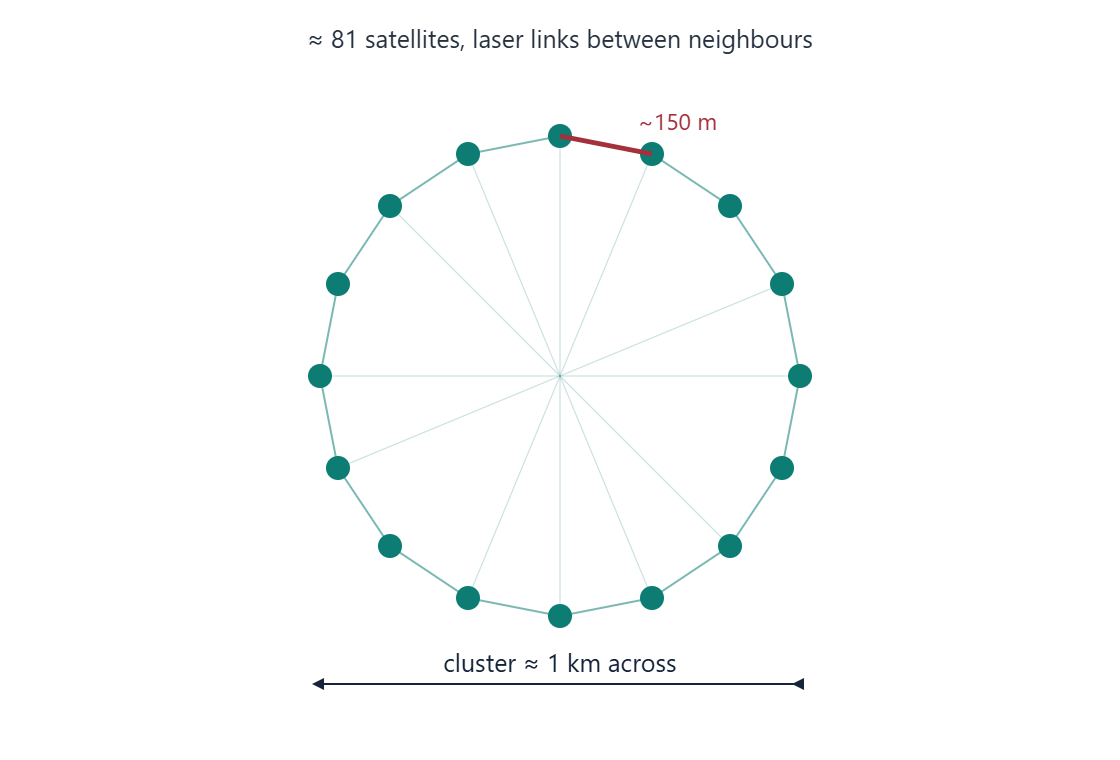
\includegraphics[keepaspectratio,alt={Top view of the reference cluster: about eighty satellites within a one-kilometre circle, linked by laser at roughly one hundred and fifty metre spacing.}]{schematics/diagram_constellation.png}}
\caption{Top view of the reference cluster: about eighty satellites
within a one-kilometre circle, linked by laser at roughly one hundred
and fifty metre spacing.}
\end{figure}

Throughout this analysis the reference design follows the Suncatcher
parameters: a dawn-dusk sun-synchronous orbit at 650 km, an
eighty-one-satellite cluster of one-kilometer radius, and
inter-satellite spacing of roughly 150 m. The reference satellite bus is
taken to carry four accelerators with an avionics and support
complement, consistent with the mass budget developed in Chapter 12.
Where the analysis examines higher-power chips (NVIDIA H100 at 700 W,
B200 at 1000 W, the GB200 GPU at 1200 W), it does so to test the scaling
of each subsystem, because the trend in AI accelerators is toward
higher, not lower, per-chip power.

The scope of the models is conceptual to preliminary design (Phase A in
aerospace terms). The intent is to size each subsystem, rank the risks,
and quantify the trades, not to produce a certifiable flight design.
Several domains are treated at first order with explicit uncertainty
bands, and a number of analyses that a flight program would require (a
thermal finite-element model, a closed-loop attitude-control simulation,
formal failure-modes analysis, and runs of the official agency debris
and radiation tools) are out of scope and are identified as such in
Chapter 24. Stating the fidelity plainly is essential: the value of the
model lies in its breadth and its transparency, not in a claim of flight
accuracy.

\begin{center}\rule{0.5\linewidth}{0.5pt}\end{center}

\textbf{Cluster geometry and inter-satellite spacing.} The reference
cluster places \(N\) satellites within a disc of radius \(R\), and the
chosen figures are \(N = 81\) and \(R = 1\ \mathrm{km}\). If the
satellites are distributed so that each occupies an equal share of the
disc area, the area per satellite is the total area divided by the
count,

\begin{equation}
A_{\mathrm{sat}} = \frac{\pi R^{2}}{N}. \tag{3.1}
\end{equation}

A convenient single length scale for a uniform planar arrangement is the
side of the square that contains this area, which gives the
characteristic spacing

\begin{equation}
s \;=\; \sqrt{A_{\mathrm{sat}}} \;=\; R\,\sqrt{\frac{\pi}{N}}. \tag{3.2}
\end{equation}

Substituting the reference values,
\(s = (1000\ \mathrm{m})\sqrt{\pi/81} = (1000\ \mathrm{m})\,(1.772/9) \approx 197\ \mathrm{m}\),
which is the same order as the quoted nearest-neighbour spacing of
roughly \(150\ \mathrm{m}\); the difference reflects that nearest
neighbours sit closer than the area-equivalent square edge, since a
hexagonal close packing reduces the nearest-neighbour distance by a
factor near \(\sqrt{2/\sqrt{3}}\) relative to the square cell. The
design implication is that station-keeping and collision-avoidance
budgets must hold relative position to a small fraction of \(s\), so the
control authority required scales inversely with the spacing the
architecture selects.

\textbf{Orbital period and ground-track repetition.} At the reference
altitude \(h = 650\ \mathrm{km}\) the orbital radius is
\(a = R_{\oplus} + h\), and the Keplerian period follows from equating
gravitational and centripetal acceleration, \(\mu/a^{2} = \omega^{2} a\)
with \(\omega = 2\pi/T\), which rearranges to

\begin{equation}
T = 2\pi\,\sqrt{\frac{a^{3}}{\mu}}, \tag{3.3}
\end{equation}

where \(\mu\) is the Earth gravitational parameter. The dawn-dusk
sun-synchronous condition then fixes the orbital plane precession rate
\(\dot{\Omega}\) to match the mean motion of the Earth about the Sun,
\(\dot{\Omega} = 2\pi / (1\ \mathrm{yr})\), through the nodal-regression
relation

\begin{equation}
\dot{\Omega} = -\frac{3}{2}\,J_{2}\left(\frac{R_{\oplus}}{a}\right)^{2}\,n\,\cos i, \tag{3.4}
\end{equation}

with \(n = 2\pi/T\) the mean motion, \(J_{2}\) the dominant geopotential
coefficient, and \(i\) the inclination. Equation (3.4) shows that for a
prescribed altitude only one inclination, slightly retrograde, satisfies
the sun-synchronous constraint. The design implication is that altitude
and inclination are not independent choices: once \(h\) is set for the
cluster, the dawn-dusk illumination that keeps the radiators in shadow
and the arrays in near-continuous sunlight dictates \(i\), and any later
altitude trade reopens the attitude and power geometry together.

\chapter{3A. Design Methodology, Margins, and
Readiness}\label{a.-design-methodology-margins-and-readiness}

\begin{quote}
\emph{Abstract.} This chapter sets the design discipline: the
mass-growth and power allowances drawn from established flight practice,
and an explicit technology-readiness assessment that locates each
capability on the nine-level scale.
\end{quote}

\emph{Sources: margin and readiness practice from the NASA Systems
Engineering Handbook {[}13{]}, AIAA S-120 {[}14{]}, the Goddard
concurrent-design practice {[}15{]}, and the SMAD systems text
{[}18{]}.}

A conceptual design is judged not only by its point estimates but by the
allowances it carries against growth and uncertainty. This analysis
follows the practice of the NASA Systems Engineering Handbook
(NASA/SP-2016-6105), which tracks resource margins as technical
performance measures rather than prescribing fixed numbers, together
with the quantitative allowances that flight programs apply.

\textbf{Mass growth.} AIAA S-120-2006 sets a mass-growth allowance by
hardware category for an estimated design: 30 percent for small
electronics and solar arrays, 25 percent for structures, mechanisms,
thermal control, batteries, and propulsion, 20 percent for large
electronics, and 60 percent for harness. On top of the per-item
allowance, the NASA Goddard Integrated Design Center applies a
system-level mass margin of about 30 percent at the pre-Phase-A concept
stage. Published mass-growth data from operational programs show actual
growth often exceeds the AIAA allowance, so these figures are treated as
lower bounds. The reference dry mass reported in Chapter 12 is a
current-best-estimate; applying the allowances above (implemented in the
margins module) gives the predicted mass a program would budget.

\textbf{Power.} The Goddard practice sizes the power system for a
minimum 30 percent contingency of delivered power over the
current-best-estimate load, evaluated at the worst-case operational
scenario at end of life. The dawn-dusk power margin of Chapter 11 is
interpreted against this rule.

\textbf{Readiness.} Progress is measured on the NASA nine-level
technology-readiness scale, from basic principles observed (level 1) to
a system flight-proven through successful operations (level 9). The
components of the reference architecture sit near the middle: a single
accelerator has operated in orbit and a processor has been ground-tested
for radiation (component levels 5 to 6), while the constellation-scale
system, the flown multi-terabit formation links, and validated formation
station-keeping remain at low system readiness. The gap between
component and system readiness is the central programmatic risk
identified in Chapter 23. Assessing each major capability against the
nine-level scale makes that gap explicit.

{\def\LTcaptype{none} % do not increment counter
\begin{longtable}[]{@{}
  >{\raggedright\arraybackslash}p{(\linewidth - 6\tabcolsep) * \real{0.2500}}
  >{\raggedright\arraybackslash}p{(\linewidth - 6\tabcolsep) * \real{0.2500}}
  >{\raggedright\arraybackslash}p{(\linewidth - 6\tabcolsep) * \real{0.2500}}
  >{\raggedright\arraybackslash}p{(\linewidth - 6\tabcolsep) * \real{0.2500}}@{}}
\toprule\noalign{}
\begin{minipage}[b]{\linewidth}\raggedright
Capability
\end{minipage} & \begin{minipage}[b]{\linewidth}\raggedright
Demonstrated status, 2026
\end{minipage} & \begin{minipage}[b]{\linewidth}\raggedright
Assessed TRL
\end{minipage} & \begin{minipage}[b]{\linewidth}\raggedright
Gating step to the next level
\end{minipage} \\
\midrule\noalign{}
\endhead
\bottomrule\noalign{}
\endlastfoot
Data-center-class accelerator in orbit & one GPU flown (Starcloud-1, Nov
2025) & 6 & sustained multi-unit operation on orbit \\
Processor radiation tolerance & ground-tested, no hard failures to 15
krad & 5 & in-flight dose and upset-rate confirmation \\
Node-level thermal control & kilowatt-class pumped-loop nodes flown & 5
& a megawatt-class radiator flown \\
Multi-terabit formation optical link & bench-scale link only & 4 & a
flown link between two satellites \\
Formation station-keeping at sub-km spacing & not demonstrated & 3 &
two-satellite close-formation flight \\
Autonomous cluster debris avoidance & not demonstrated & 2 & a
closed-loop avoidance maneuver on orbit \\
Propulsive disposal within five years & components flight-proven,
configuration unproven & 5 & an end-to-end de-orbit demonstration \\
Megawatt-to-gigawatt cluster & conceptual & 2 & a subscale
multi-satellite cluster \\
\end{longtable}
}

The assessment confirms the central pattern: the building blocks sit at
component levels 4 to 6, while every capability that depends on the
constellation operating as a coordinated system sits at levels 2 to 3.
The program risk is concentrated in the system-integration steps, not
the components.

{\def\LTcaptype{none} % do not increment counter
\begin{longtable}[]{@{}
  >{\raggedright\arraybackslash}p{(\linewidth - 4\tabcolsep) * \real{0.3333}}
  >{\raggedright\arraybackslash}p{(\linewidth - 4\tabcolsep) * \real{0.3333}}
  >{\raggedright\arraybackslash}p{(\linewidth - 4\tabcolsep) * \real{0.3333}}@{}}
\toprule\noalign{}
\begin{minipage}[b]{\linewidth}\raggedright
Allowance
\end{minipage} & \begin{minipage}[b]{\linewidth}\raggedright
Value
\end{minipage} & \begin{minipage}[b]{\linewidth}\raggedright
Source
\end{minipage} \\
\midrule\noalign{}
\endhead
\bottomrule\noalign{}
\endlastfoot
Mass growth, small electronics and solar array & 30 percent & AIAA
S-120-2006 \\
Mass growth, structures, thermal, battery, propulsion & 25 percent &
AIAA S-120-2006 \\
Mass growth, large electronics & 20 percent & AIAA S-120-2006 \\
Mass growth, harness & 60 percent & AIAA S-120-2006 \\
System-level mass margin, pre-Phase-A & 30 percent & NASA GSFC
Integrated Design Center \\
Power contingency over best estimate, worst-case end of life & 30
percent minimum & NASA GSFC Integrated Design Center \\
Readiness framework & levels 1 to 9 & NASA Systems Engineering Handbook,
NASA/SP-2016-6105 \\
\end{longtable}
}

\begin{center}\rule{0.5\linewidth}{0.5pt}\end{center}

\textbf{Composing the mass allowances.} The allowances quoted above act
multiplicatively on a current-best-estimate, not additively across the
system. Let \(m_i\) be the current-best-estimate mass of hardware item
\(i\) and let \(g_i\) be the AIAA S-120 growth fraction for that item's
category. The predicted, or maximum-expected, mass of the item is

\begin{equation}
m_i^{\,\mathrm{pred}} = m_i\,(1 + g_i). \tag{3A.1}
\end{equation}

Summing over the parts list gives the predicted dry mass before any
system-level reserve,

\begin{equation}
M_{\mathrm{dry}}^{\,\mathrm{pred}} = \sum_i m_i\,(1 + g_i). \tag{3A.2}
\end{equation}

The system-level mass margin of the Goddard practice is then applied on
top of the aggregated prediction, so the mass a program would budget is

\begin{equation}
M_{\mathrm{budget}} = (1 + M_{\mathrm{sys}})\sum_i m_i\,(1 + g_i), \tag{3A.3}
\end{equation}

with \(M_{\mathrm{sys}} = 0.30\) at the pre-Phase-A stage. It is
convenient to express the combined effect as an effective system growth
fraction relative to the raw estimate \(M_0 = \sum_i m_i\),

\begin{equation}
G_{\mathrm{eff}} = \frac{M_{\mathrm{budget}}}{M_0} - 1 = (1 + M_{\mathrm{sys}})\,\frac{\sum_i m_i\,(1 + g_i)}{\sum_i m_i} - 1, \tag{3A.4}
\end{equation}

in which the fraction is the mass-weighted average of \((1 + g_i)\).
Because the per-item term and the system reserve compound,
\(G_{\mathrm{eff}}\) exceeds the simple sum of the two contributions.

\textbf{Worked example.} Consider a notional item set whose
current-best-estimate mass is dominated by structure carrying
\(g = 0.25\), so the mass-weighted average of \((1 + g_i)\) is close to
\(1.25\). Applying the system reserve of (3A.3),

\begin{equation}
G_{\mathrm{eff}} \approx (1.30)(1.25) - 1 = 0.625, \tag{3A.5}
\end{equation}

an effective allowance near 62 percent over the raw estimate, well above
the 30 percent system reserve taken alone. This is the figure a designer
should hold in mind when reserving launch capacity.

\textbf{Power contingency at end of life.} The power rule is a
worst-case inequality rather than a point sizing. Writing
\(P_{\mathrm{gen}}^{\mathrm{EOL}}\) for the array power delivered at end
of life in the worst-case operational geometry, and
\(P_{\mathrm{load}}\) for the current-best-estimate load, the
contingency requirement is

\begin{equation}
\frac{P_{\mathrm{gen}}^{\mathrm{EOL}} - P_{\mathrm{load}}}{P_{\mathrm{load}}} \ge C_P, \qquad C_P = 0.30. \tag{3A.6}
\end{equation}

Equivalently the array must be sized so that
\(P_{\mathrm{gen}}^{\mathrm{EOL}} \ge (1 + C_P)\,P_{\mathrm{load}}\).
Since the array degrades over the mission, the beginning-of-life
requirement is larger by the inverse of the survival fraction
\(\eta_{\mathrm{deg}} = P_{\mathrm{gen}}^{\mathrm{EOL}}/P_{\mathrm{gen}}^{\mathrm{BOL}}\),

\begin{equation}
P_{\mathrm{gen}}^{\mathrm{BOL}} \ge \frac{(1 + C_P)\,P_{\mathrm{load}}}{\eta_{\mathrm{deg}}}. \tag{3A.7}
\end{equation}

The design implication is that contingency and degradation stack: the
array must be oversized at deployment by both the 30 percent reserve and
the reciprocal of its end-of-life survival fraction, and the dawn-dusk
margin of Chapter 11 should be checked against the worst-case
end-of-life form of (3A.6), not against a beginning-of-life value.

\part{THE ORBITAL ENVIRONMENT}\label{the-orbital-environment}

\chapter{4. Orbital Mechanics of a Circular
Orbit}\label{orbital-mechanics-of-a-circular-orbit}

\begin{quote}
\emph{Abstract.} This chapter derives the small set of circular-orbit
quantities, speed, period, and specific energy, on which every later
chapter depends, and works the reference orbit as an example.
\end{quote}

\emph{Sources: the circular-orbit relations, vis-viva equation, and
specific energy follow standard astrodynamics texts, principally Curtis
{[}16{]} and Vallado {[}17{]}.}

Every subsequent chapter depends on a small set of orbital quantities,
derived here.

\textbf{Circular speed.} For a satellite of mass \(m\) on a circular
orbit of radius \(a\), gravity supplies the centripetal force:

\begin{equation}
\frac{\mu m}{a^2} = \frac{m v^2}{a} \quad\Longrightarrow\quad v = \sqrt{\frac{\mu}{a}}. \tag{4.1}
\end{equation}

\textbf{Period and mean motion.} From \(v = 2\pi a / T\),

\begin{equation}
T = 2\pi\sqrt{\frac{a^3}{\mu}}, \qquad n = \frac{2\pi}{T} = \sqrt{\frac{\mu}{a^3}}. \tag{4.2}
\end{equation}

\textbf{Vis-viva and specific energy.} For a general orbit, energy
conservation yields the vis-viva relation
\(v^2 = \mu\left(\tfrac{2}{r} - \tfrac{1}{a}\right)\), and the total
specific energy is

\begin{equation}
\mathcal{E} = \frac{v^2}{2} - \frac{\mu}{r} = -\frac{\mu}{2a}. \tag{4.3}
\end{equation}

Equation (4.3) is the key to the orbital-decay derivation in Chapter 7:
drag removes energy, and a loss of energy means a more negative
\(\mathcal{E}\), hence a smaller \(a\).

\textbf{The two-body problem.} The circular relations above are special
cases of the two-body problem. Newton's law of gravitation and the
second law give the relative acceleration of the satellite with respect
to Earth,

\begin{equation}
\ddot{\mathbf r} = -\frac{\mu}{r^{3}}\,\mathbf r, \qquad \mu = G(M_\oplus + m) \approx G M_\oplus, \tag{4.4}
\end{equation}

where the approximation holds because the satellite mass is negligible
against Earth's. Taking the cross product of (4.4) with \(\mathbf r\)
shows that the specific angular momentum is conserved,

\begin{equation}
\mathbf h = \mathbf r \times \dot{\mathbf r}, \qquad \frac{d\mathbf h}{dt} = 0, \tag{4.5}
\end{equation}

so the motion stays in a plane and the radius vector sweeps equal areas
in equal times, which is Kepler's second law.

\textbf{The orbit equation.} Integrating (4.4) once, using the conserved
eccentricity (Laplace-Runge-Lenz) vector, yields the trajectory as a
conic section written in focal polar form,

\begin{equation}
r(\theta) = \frac{h^{2}/\mu}{1 + e\cos\theta} = \frac{p}{1 + e\cos\theta}, \qquad p = a\left(1 - e^{2}\right), \tag{4.6}
\end{equation}

where \(e\) is the eccentricity, \(\theta\) the true anomaly measured
from perigee, and \(p\) the semi-latus rectum. Bound orbits have
\(0 \le e < 1\); the circular orbit used throughout this study is the
special case \(e = 0\), for which \(r = a\) is constant and (4.1) to
(4.3) follow directly.

\textbf{Kepler's third law.} For an ellipse of semi-axes \(a\) and
\(b = a\sqrt{1-e^{2}}\), the constant areal rate \(\dot A = h/2\)
integrated over the enclosed area \(\pi a b\) gives the period

\begin{equation}
T = 2\pi\sqrt{\frac{a^{3}}{\mu}}, \tag{4.7}
\end{equation}

independent of eccentricity, which is why the circular result (4.2)
applies to the slightly non-circular reference orbit without correction.

\textbf{Ground track and revisit.} Coverage planning needs the ground
track, the locus of sub-satellite points. While the satellite completes
one orbit in time \(T\), Earth turns beneath it at
\(\omega_\oplus = 7.292\times10^{-5}\) rad/s, so successive equator
crossings step westward by \(\Delta\lambda = \omega_\oplus T\). A ground
track repeats when an integer number of orbits \(k\) fills an integer
number \(d\) of nodal days, \(k\,T = d\,(2\pi/\omega_\oplus)\); for the
reference orbit \(\Delta\lambda \approx 24.4^\circ\) per revolution, and
the near-15-orbit day sets the natural revisit cadence over a given
ground station (Chapter 14).

\textbf{Worked example.} At \(h = 650\) km,
\(a = R_E + h = 7.021\times10^6\) m:

\[v = \sqrt{\frac{3.986\times10^{14}}{7.021\times10^6}} = 7534.8\ \mathrm{m/s}, \qquad
T = 2\pi\sqrt{\frac{(7.021\times10^6)^3}{3.986\times10^{14}}} = 5854.8\ \mathrm{s} = 97.6\ \mathrm{min}.\]

The orbital speed is about 7.5 km/s and the period about 97.6 minutes,
giving roughly 14.8 orbits per day. These values are reproduced exactly
by \passthrough{\lstinline!orbital\_dc.orbit.velocity(650)!} and
\passthrough{\lstinline!period(650)!}.

\chapter{5. Sun-Synchronous Orbits and J2
Precession}\label{sun-synchronous-orbits-and-j2-precession}

\begin{quote}
\emph{Abstract.} This chapter derives the secular nodal precession
caused by Earth's oblateness and the inclination that makes an orbit
sun-synchronous, and confirms the reference value of about ninety-eight
degrees.
\end{quote}

\begin{figure}
\centering
\pandocbounded{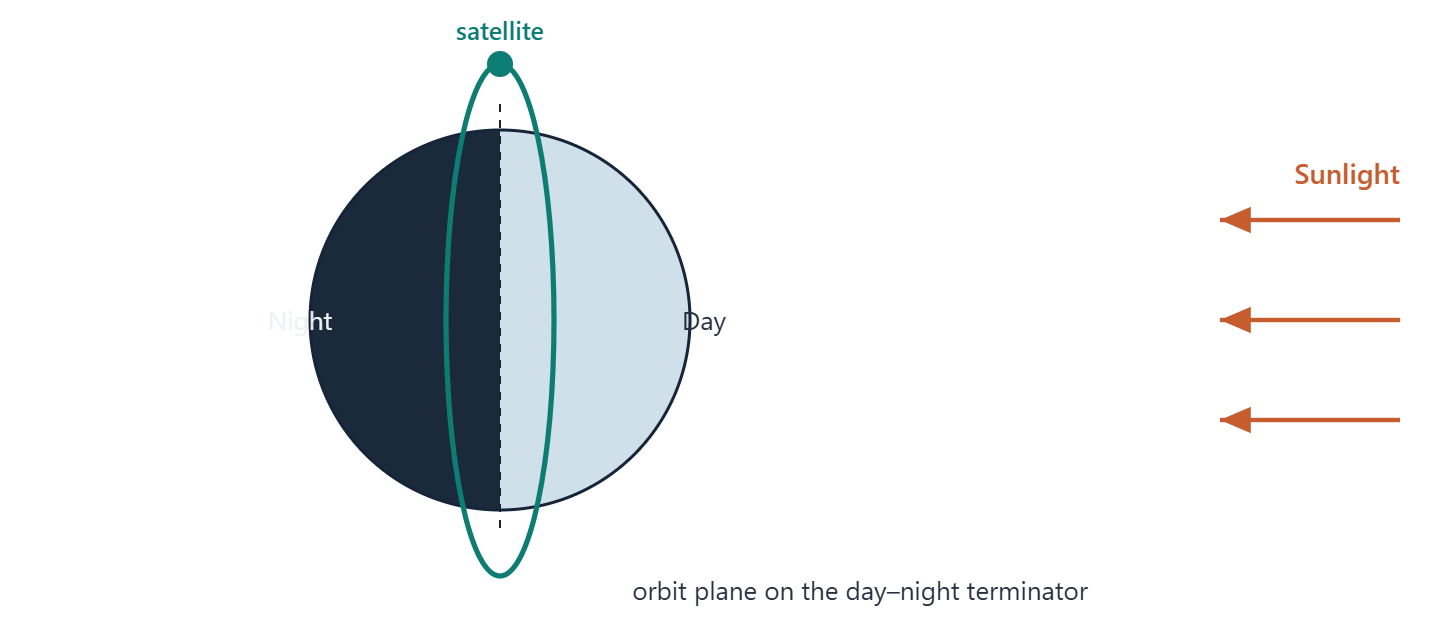
\includegraphics[keepaspectratio,alt={The dawn-dusk sun-synchronous orbit, with the orbital plane held on the day-night terminator so the satellite stays sunlit.}]{schematics/diagram_orbit.png}}
\caption{The dawn-dusk sun-synchronous orbit, with the orbital plane
held on the day-night terminator so the satellite stays sunlit.}
\end{figure}

\emph{Sources: the J2 secular precession and the sun-synchronous
condition follow Vallado {[}17{]} and Curtis {[}16{]}.}

A sun-synchronous orbit maintains a near-constant orientation relative
to the Sun by exploiting Earth's oblateness. The dominant non-spherical
term in Earth's gravity, characterized by \(J_2\), causes the orbital
plane's right ascension of the ascending node, \(\Omega\), to precess.
The secular precession rate for a near-circular orbit is

\begin{equation}
\dot\Omega = -\frac{3}{2}\, n\, J_2 \left(\frac{R_E}{a}\right)^2 \cos i. \tag{5.1}
\end{equation}

\textbf{Origin of the precession.} Earth's gravitational potential,
expanded in zonal harmonics and kept to the leading oblateness term, is

\begin{equation}
U(r,\phi) = -\frac{\mu}{r}\left[\,1 - J_2\left(\frac{R_E}{r}\right)^2 P_2(\sin\phi)\,\right],
\qquad P_2(\sin\phi) = \tfrac{1}{2}\left(3\sin^2\phi - 1\right), \tag{5.2}
\end{equation}

where \(\phi\) is geocentric latitude and \(P_2\) is the second Legendre
polynomial. The term beyond the point-mass field is the disturbing
function \(R\). Writing the latitude through the orbital geometry,
\(\sin\phi = \sin i\,\sin(\omega + \theta)\) with \(\theta\) the true
anomaly, and averaging \(R\) over one revolution removes the
short-period terms and leaves the secular part

\begin{equation}
\bar R = \frac{n^2 J_2 R_E^2}{2}\,\frac{1}{(1-e^2)^{3/2}}
\left(\frac{3}{2}\sin^2 i - 1\right). \tag{5.3}
\end{equation}

Lagrange's planetary equation for the node connects this averaged
potential to the drift of \(\Omega\),

\begin{equation}
\dot\Omega = \frac{1}{n a^2 \sqrt{1-e^2}\,\sin i}\,\frac{\partial \bar R}{\partial i}. \tag{5.4}
\end{equation}

Carrying out the derivative of (5.3) with respect to \(i\) gives
\(\partial\bar R/\partial i \propto \sin i\cos i\), and the \(\sin i\)
in the denominator of (5.4) cancels, leaving the \(\cos i\) dependence
of (5.1). The result is exact at first order in \(J_2\) for any
eccentricity if \(a\) is replaced by the semi-latus rectum
\(p = a(1-e^2)\); for the near-circular reference orbit \(p \approx a\)
and (5.1) follows directly. The sign is negative for prograde orbits
(\(i < 90^\circ\)), so the node regresses, and positive for retrograde
orbits, which is what makes synchronization with the Sun possible.

A sun-synchronous orbit chooses the inclination \(i\) so that this
precession equals Earth's mean rate about the Sun,
\(\dot\Omega_{\mathrm{sun}} = 2\pi / (365.2422\ \mathrm{d}) = 1.991\times10^{-7}\ \mathrm{rad/s}\).
Setting \(\dot\Omega = \dot\Omega_{\mathrm{sun}}\) and solving,

\begin{equation}
\cos i = -\frac{2\,\dot\Omega_{\mathrm{sun}}\, a^2}{3\, n\, J_2\, R_E^2}. \tag{5.5}
\end{equation}

The negative sign forces \(i > 90^\circ\), a retrograde, near-polar
orbit. At 650 km, \(n = 1.074\times10^{-3}\ \mathrm{rad/s}\) and (5.5)
gives \(\cos i = -0.139\), hence \(i = 98.0^\circ\), matching the
reference mission and the value returned by
\passthrough{\lstinline!orbital\_dc.orbit.sso\_inclination(650)!}. By
construction the corresponding nodal precession is \(0.9856\) degrees
per day, exactly one turn per tropical year, which is the defining
property of the orbit. The required inclination rises slowly with
altitude, from about \(96.3^\circ\) at 200 kilometers to \(98.6^\circ\)
at 800 kilometers, because the \(a^2\) factor in (5.5) outpaces the fall
in \(n\). The dawn-dusk variant orients the orbital plane near Earth's
terminator, which (Chapter 6) yields nearly continuous sunlight and
minimal thermal cycling, a decisive advantage for a high-power,
thermally sensitive payload.

\textbf{Recovering the mean motion.} The precession rate (5.1) and the
inclination condition (5.5) both require the mean motion \(n\), which
follows from Kepler's third law for a two-body orbit. Equating the
gravitational force to the centripetal requirement for a circular orbit
of radius \(a\), \(\mu m / a^2 = m\, n^2 a\), gives the relation between
angular rate and size,

\begin{equation}
n = \sqrt{\frac{\mu}{a^3}}, \tag{5.6}
\end{equation}

where \(\mu = G M_E\) is Earth's gravitational parameter and
\(a = R_E + h\) for a circular orbit at altitude \(h\). The orbital
period is then \(T = 2\pi / n = 2\pi\sqrt{a^3/\mu}\). Because \(n\)
scales as \(a^{-3/2}\), doubling the altitude lengthens the period and
slows the satellite, which is the falling factor that competes with the
rising \(a^2\) term in (5.5).

\textbf{The worked inclination at the reference altitude.} Take the
reference orbit at \(h = 650\) km, so
\(a = R_E + h \approx 6378 + 650 = 7028\) km. Substituting into (5.6)
with \(\mu = 3.986\times10^{14}\ \mathrm{m^3/s^2}\) returns
\(n = 1.074\times10^{-3}\ \mathrm{rad/s}\), the value already quoted in
the chapter. Feeding this \(n\), together with
\(J_2 = 1.083\times10^{-3}\) and \(R_E = 6378\) km, into the
synchronization condition (5.5) yields \(\cos i = -0.139\), hence
\(i = 98.0^\circ\), in agreement with the reference mission. The two
relations therefore form a closed chain: altitude fixes \(n\) through
(5.6), and \(n\) fixes the inclination through (5.5).

\textbf{Sensitivity to altitude.} Differentiating (5.5) shows how
tightly the inclination must be held as the altitude is chosen. Writing
\(\cos i \propto a^2 / n = a^2 a^{3/2} = a^{7/2}\) after inserting
(5.6), the synchronization condition becomes

\begin{equation}
\cos i = -\frac{2\,\dot\Omega_{\mathrm{sun}}}{3\, J_2\, R_E^2}\,\frac{a^{7/2}}{\sqrt{\mu}}, \tag{5.7}
\end{equation}

which makes explicit the strong \(a^{7/2}\) growth that drives \(i\)
from \(96.3^\circ\) toward \(98.6^\circ\) across the low-Earth-orbit
band. The design implication is that the sun-synchronous inclination is
a slowly varying but firmly dictated function of the chosen altitude;
once a thermal or power requirement sets the altitude, the inclination
is not a free parameter but is fixed to within a small fraction of a
degree by (5.7).

\chapter{6. Eclipse Geometry and the Dawn-Dusk
Advantage}\label{eclipse-geometry-and-the-dawn-dusk-advantage}

\begin{quote}
\emph{Abstract.} This chapter derives the beta angle and the sunlit
fraction of the orbit from the cylindrical-shadow geometry, and shows
why the dawn-dusk orbit stays sunlit year round.
\end{quote}

\begin{figure}
\centering
\pandocbounded{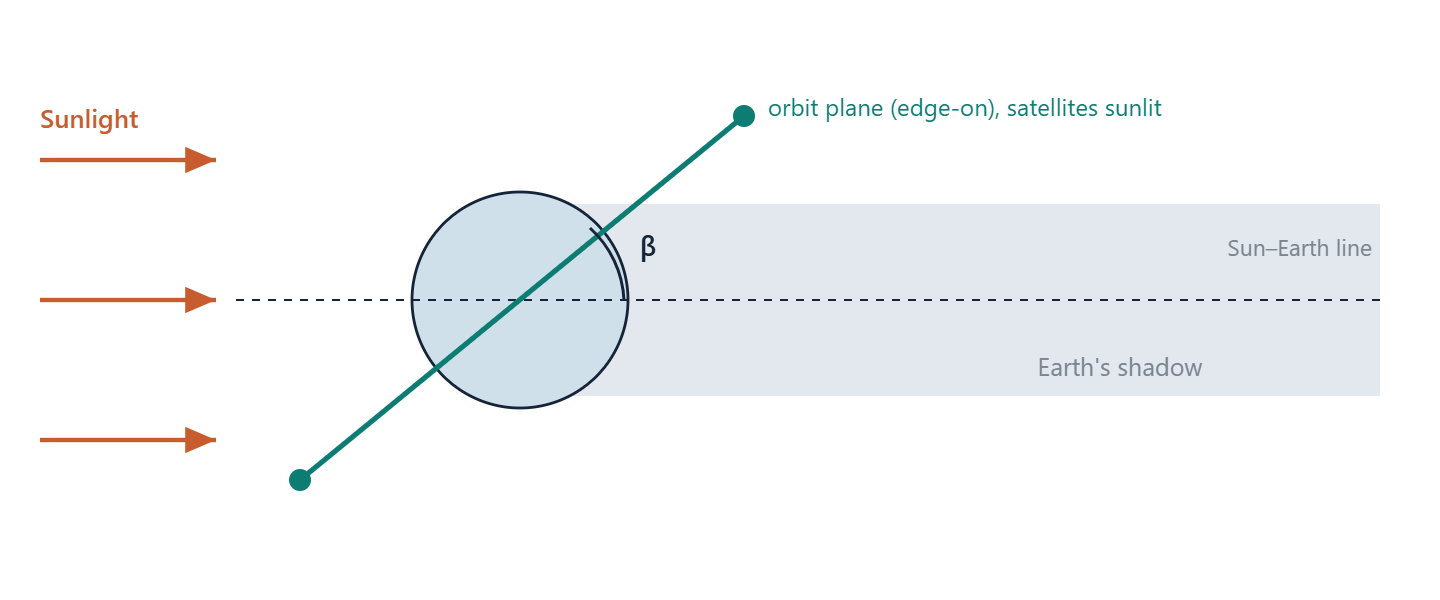
\includegraphics[keepaspectratio,alt={The beta angle between the orbit plane and the Sun line, set against Earth's shadow; a high beta keeps the orbit out of eclipse.}]{schematics/diagram_beta.png}}
\caption{The beta angle between the orbit plane and the Sun line, set
against Earth's shadow; a high beta keeps the orbit out of eclipse.}
\end{figure}

\emph{Sources: the beta-angle and eclipse-fraction geometry follow
Curtis {[}16{]} and the SMAD mission-design text {[}18{]}.}

The fraction of each orbit spent in Earth's shadow is set by the beta
angle \(\beta\), the angle between the orbital plane and the Sun line. A
satellite avoids eclipse entirely when \(|\beta|\) exceeds the critical
value at which the orbit just grazes Earth's limb:

\begin{equation}
\beta^{*} = \arcsin\!\left(\frac{R_E}{R_E + h}\right). \tag{6.1}
\end{equation}

For \(|\beta| < \beta^{*}\), the sunlit fraction of the orbit is

\begin{equation}
f_{\mathrm{sun}} = 1 - \frac{1}{\pi}\cos^{-1}\!\left[\frac{\sqrt{h^2 + 2 R_E h}}{(R_E + h)\cos\beta}\right]. \tag{6.2}
\end{equation}

\textbf{Derivation from the cylindrical shadow.} Treat Earth's shadow as
a half-infinite cylinder of radius \(R_E\) pointing away from the Sun, a
good approximation in low Earth orbit where the penumbra is narrow and
the Sun is effectively at infinity. A point on the circular orbit of
radius \(r = R_E + h\) lies in shadow when its distance from the shadow
axis is less than \(R_E\) and it is on the anti-sun side. Resolve the
orbit into the shadow frame: the component of the orbit radius
perpendicular to the Sun line, for an orbit whose plane makes angle
\(\beta\) with that line, traces an ellipse of semi-axes \(r\) and
\(r\cos\beta\). The satellite is eclipsed over the arc where this
projected position falls within the cylinder, and the half-angle
\(\psi\) of that arc, measured from the anti-solar point, satisfies

\begin{equation}
\cos\psi = \frac{\sqrt{r^2 - R_E^2}}{r\,\cos\beta}
          = \frac{\sqrt{h^2 + 2 R_E h}}{(R_E + h)\cos\beta}. \tag{6.3}
\end{equation}

The eclipse occupies the fraction \(f_E = \psi/\pi\) of the orbit (the
full eclipsed arc is \(2\psi\) out of \(2\pi\)), and the sunlit fraction
is \(f_{\mathrm{sun}} = 1 - f_E\), which is (6.2). The expression is
real only while the bracket does not exceed one; the threshold where
\(\cos\psi = 1\) recovers the critical beta of (6.1), at which the
eclipse arc shrinks to zero.

\textbf{Annual variation of the beta angle.} The beta angle is not
fixed: it depends on the angle between the orbit plane and the
instantaneous Sun direction. For an orbit of inclination \(i\) and node
\(\Omega\), with solar ecliptic longitude \(\lambda_\odot\) and
obliquity \(\varepsilon = 23.44^\circ\),

\begin{equation}
\sin\beta = \cos\lambda_\odot\sin\Omega\sin i
           - \sin\lambda_\odot\cos\varepsilon\cos\Omega\sin i
           + \sin\lambda_\odot\sin\varepsilon\cos i. \tag{6.4}
\end{equation}

A sun-synchronous orbit holds \(\Omega\) at a fixed local time by
construction, so the seasonal swing of \(\lambda_\odot\) is what moves
\(\beta\). For the dawn-dusk case, where the node is set near the six
o'clock line so the orbit plane contains the terminator, (6.4) reduces
to \(|\beta|\) oscillating between about \(66.6^\circ\) and \(90^\circ\)
over the year, the lower bound being \(90^\circ - \varepsilon\).

At 650 km, \(\beta^{*} = \arcsin(6371/7021) = 65.1^\circ\). Because the
dawn-dusk orbit keeps \(|\beta|\) above \(66.6^\circ\) at all times, it
stays above this \(65.1^\circ\) threshold year round, so the satellite
never enters a deep eclipse and \(f_{\mathrm{sun}} \to 1\): illumination
exceeds ninety-five percent, the battery need is minimal (Chapter 11),
and the thermal environment is nearly steady, justifying the
quasi-steady thermal treatment of Chapter 10. This is the single most
favorable environmental choice available to the architecture, and it is
robust to the seasonal beta swing rather than dependent on a single
favorable date.

\begin{figure}
\centering
\pandocbounded{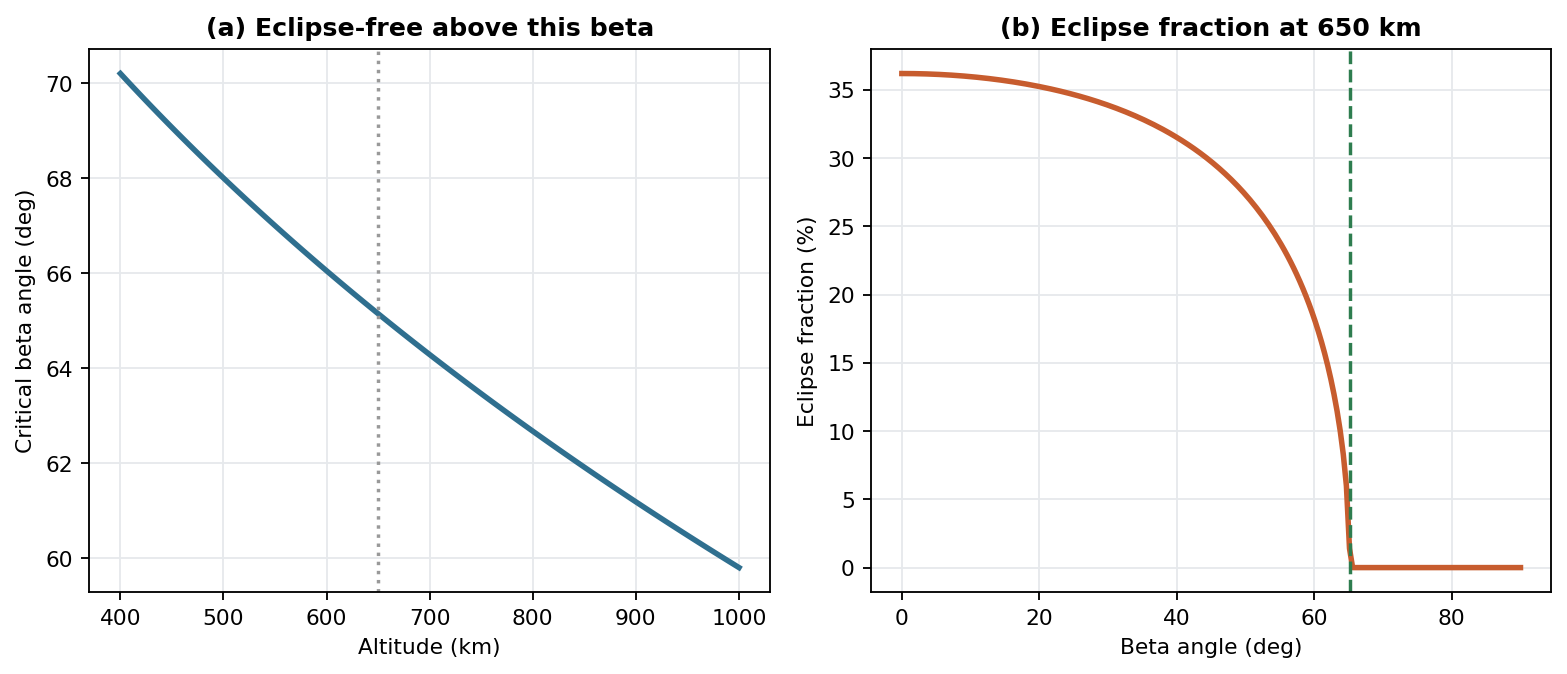
\includegraphics[keepaspectratio,alt={Fig. 6.1 Critical beta angle versus altitude, and eclipse fraction versus beta at 650 km. A dawn-dusk orbit holds the beta angle high, so the satellite stays sunlit.}]{figures2/figA1_eclipse.png}}
\caption{Fig. 6.1 Critical beta angle versus altitude, and eclipse
fraction versus beta at 650 km. A dawn-dusk orbit holds the beta angle
high, so the satellite stays sunlit.}
\end{figure}

\textbf{Detailed reduction of the projected geometry.} It is worth
retracing how the shadow-cylinder condition of (6.3) emerges from
vectors, because the same projection underlies the power and thermal
budgets of later chapters. Place the origin at Earth's center and let
\(\hat{\mathbf{s}}\) be the unit vector toward the Sun. A point on the
circular orbit is \(\mathbf{r}(u) = r\,\hat{\mathbf{e}}(u)\), where
\(u\) is the argument measured from the ascending point of the orbit and
\(\hat{\mathbf{e}}\) sweeps the orbit plane. The component of
\(\mathbf{r}\) along the Sun line is
\(r_\parallel = \mathbf{r}\cdot\hat{\mathbf{s}}\), and the perpendicular
distance from the shadow axis is

\begin{equation}
d_\perp(u) = \sqrt{r^2 - (\mathbf{r}\cdot\hat{\mathbf{s}})^2}. \tag{6.5}
\end{equation}

By the definition of the beta angle, the orbit plane is tilted so that
the projection of \(\mathbf{r}\) onto the Sun line has amplitude
\(r\cos\beta\) over a revolution; writing the in-plane phase as
\(\theta\) measured from the sub-solar direction gives
\(\mathbf{r}\cdot\hat{\mathbf{s}} = r\cos\beta\,\cos\theta\), so that

\begin{equation}
d_\perp(\theta) = r\sqrt{1 - \cos^2\beta\,\cos^2\theta}. \tag{6.6}
\end{equation}

\textbf{Solving for the eclipse arc.} Eclipse requires both
\(d_\perp < R_E\) and the anti-solar half \(\cos\theta < 0\). Setting
\(d_\perp = R_E\) at the boundary and solving (6.6) for the phase
\(\theta = \pi - \psi\) at which the orbit crosses the cylinder wall,

\begin{equation}
\cos^2\beta\,\cos^2\psi = 1 - \frac{R_E^2}{r^2} = \frac{r^2 - R_E^2}{r^2}, \tag{6.7}
\end{equation}

and taking the positive root recovers
\(\cos\psi = \sqrt{r^2 - R_E^2}\,/(r\cos\beta)\), which is exactly
(6.3). The eclipse exists only when the right side of (6.7) does not
exceed \(\cos^2\beta\); the equality \(\cos\psi = 1\) reproduces
\(\cos\beta = \sqrt{r^2 - R_E^2}/r = \sqrt{1 - (R_E/r)^2}\), equivalent
to \(\sin\beta^\ast = R_E/r\) of (6.1). The two relations are therefore
one statement viewed at its limit.

\textbf{Eclipse duration in time.} For mission power sizing the arc must
be converted to a duration. The orbital period follows from Kepler's
third law,

\begin{equation}
T = 2\pi\sqrt{\frac{r^3}{\mu_\oplus}}, \tag{6.8}
\end{equation}

with \(\mu_\oplus\) the Earth gravitational parameter, and the eclipse
interval is the eclipsed fraction times the period,

\begin{equation}
t_E = \frac{2\psi}{2\pi}\,T = \frac{\psi}{\pi}\,T. \tag{6.9}
\end{equation}

\textbf{Worked example.} At \(h = 650\) km, \(r = 7021\) km and
\(\beta^\ast = 65.1^\circ\), as stated in the chapter. For the dawn-dusk
orbit the beta angle never falls below \(66.6^\circ\), so
\(|\beta| > \beta^\ast\) throughout the year; (6.7) then has no real
solution for \(\psi\), the eclipse arc vanishes, \(t_E = 0\), and the
sunlit fraction \(f_{\mathrm{sun}} \to 1\), consistent with the
chapter's statement that illumination exceeds ninety-five percent.

\textbf{Design implication.} Because the eclipse duration collapses to
zero whenever \(|\beta|\) exceeds \(\beta^\ast\), holding the dawn-dusk
node removes the eclipse load term from the power and energy-storage
budgets, so the battery is sized for contingency and load transients
rather than for nightly discharge.

\chapter{7. The Neutral Atmosphere and Orbital
Decay}\label{the-neutral-atmosphere-and-orbital-decay}

\begin{quote}
\emph{Abstract.} This chapter derives the orbital-decay rate from the
energy balance under atmospheric drag and integrates it to a mission
lifetime, a result that decides compliance with the five-year disposal
rule.
\end{quote}

\emph{Sources: density from the NRLMSIS empirical model {[}11{]}; the
drag and orbit-averaged decay treatment follows Curtis {[}16{]} and the
space-environment texts of Tribble {[}22{]} and Pisacane {[}23{]}.}

Even at 650 km a tenuous atmosphere remains, and the drag it exerts
slowly lowers the orbit. This chapter derives the decay rate and
integrates it to a mission lifetime, a result that proves decisive for
regulatory compliance.

\textbf{Drag force and specific deceleration.} A body of cross-section
\(A\) moving at speed \(v\) through gas of density \(\rho\) feels a drag
force opposing its velocity:

\begin{equation}
F_D = \tfrac{1}{2}\,\rho\, v^2\, C_D\, A, \tag{7.1}
\end{equation}

with \(C_D \approx 2.2\) in the free-molecular regime. The specific
(per-mass) deceleration is
\(a_D = F_D/m = \tfrac{1}{2}\rho v^2 C_D (A/m)\).

\textbf{Derivation of the decay rate.} Drag does negative work at the
rate (force times speed, per unit mass):

\begin{equation}
\frac{d\mathcal{E}}{dt} = -a_D\, v = -\tfrac{1}{2}\,\rho\, C_D\,\frac{A}{m}\, v^3. \tag{7.2}
\end{equation}

For a near-circular orbit \(\mathcal{E} = -\mu/2a\), so
\(d\mathcal{E}/dt = (\mu/2a^2)\,\dot a\). Equating with (7.2) and
substituting \(v = \sqrt{\mu/a}\) so that \(v^3 = (\mu/a)^{3/2}\):

\begin{equation}
\frac{\mu}{2a^2}\frac{da}{dt} = -\tfrac{1}{2}\rho C_D\frac{A}{m}\left(\frac{\mu}{a}\right)^{3/2}
\;\Longrightarrow\;
\frac{da}{dt} = -\,C_D\,\frac{A}{m}\,\rho(h)\,\sqrt{\mu\, a}. \tag{7.3}
\end{equation}

Because \(\rho(h)\) rises steeply as the orbit lowers, the decay
accelerates and terminates in a rapid re-entry. The per-revolution
contraction is \(\Delta a_{\mathrm{rev}} = \dot a\, T =
-2\pi C_D (A/m)\rho a^2\).

\textbf{Atmosphere model and solar-cycle uncertainty.} The density
\(\rho(h)\) is taken from the NRLMSIS 2.1 empirical model, interpolated
log-linearly between anchors at 600, 650, 700, and 800 km for three
levels of solar activity. The crucial feature is that density at this
altitude varies by roughly a factor of one hundred between solar minimum
and solar maximum. This single fact dominates the uncertainty in
lifetime, drag make-up, and station-keeping, and is therefore propagated
explicitly as a band rather than collapsed to a point.

\textbf{Numerical solution and result.} Equation (7.3) is integrated by
adaptive forward Euler to a re-entry altitude of 120 km. For the
reference bus, with an area-to-mass ratio of \(0.0084\ \mathrm{m^2/kg}\)
and \(C_D = 2.2\), the natural lifetime at 650 km is approximately
\textbf{twenty-two years} at moderate solar activity, about four years
at solar maximum, and over three hundred years at solar minimum (Fig.
7.1). The regulatory consequence is severe: the United States Federal
Communications Commission now requires disposal within five years
(Chapter 15), so only a satellite that happens to launch into a solar
maximum approaches passive compliance. \textbf{Active de-orbit
propulsion is therefore mandatory, not optional}, a conclusion that
propagates into the mass and economic budgets.

\begin{figure}
\centering
\pandocbounded{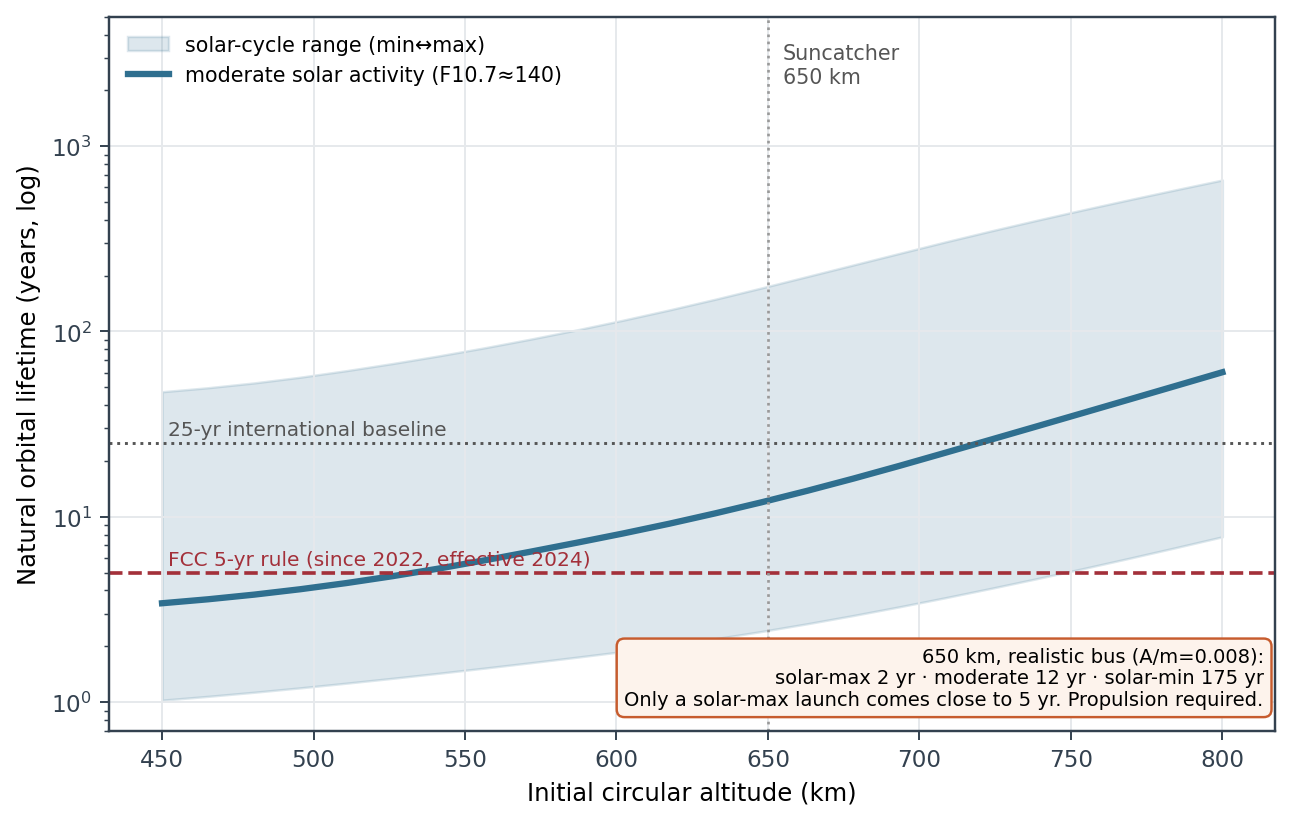
\includegraphics[keepaspectratio,alt={Fig. 7.1, Natural orbital lifetime versus altitude with the solar-cycle uncertainty band; at 650 km the realistic lifetime fails the five-year disposal rule.}]{figures/fig1_orbital_decay.png}}
\caption{Fig. 7.1, Natural orbital lifetime versus altitude with the
solar-cycle uncertainty band; at 650 km the realistic lifetime fails the
five-year disposal rule.}
\end{figure}

\textbf{Scale height and the local density gradient.} The steep altitude
dependence invoked above follows from hydrostatic balance in an
isothermal layer. Setting the upward pressure gradient against gravity,
\(dp/dh = -\rho g\), and using the ideal-gas relation
\(p = \rho k_B T / \bar m\) with mean molecular mass \(\bar m\), one
eliminates the pressure to obtain a first-order equation for the
density:

\begin{equation}
\frac{1}{\rho}\frac{d\rho}{dh} = -\frac{\bar m\, g}{k_B T} \equiv -\frac{1}{H}, \qquad H = \frac{k_B T}{\bar m\, g}. \tag{7.4}
\end{equation}

Integrating (7.4) over an interval where \(H\) is treated as constant
gives the local exponential profile

\begin{equation}
\rho(h) = \rho(h_0)\,\exp\!\left[-\frac{h - h_0}{H}\right]. \tag{7.5}
\end{equation}

The quantity \(H\) is the scale height, the vertical distance over which
density falls by a factor \(e\). This same exponential structure
justifies the log-linear interpolation between the tabulated NRLMSIS
anchors, because a straight line on a logarithmic density axis is
precisely the form of (7.5).

\textbf{Closed-form lifetime for a locally exponential atmosphere.} A
compact estimate of lifetime follows by inserting (7.5) into the decay
relation (7.3). Writing \(B = C_D (A/m)\) for the ballistic factor and
separating variables,

\begin{equation}
\frac{da}{\sqrt{a}\,\exp[-(a - a_0)/H]} = -B\,\rho_0\,\sqrt{\mu}\; dt. \tag{7.6}
\end{equation}

Because the exponential dominates the slowly varying \(\sqrt{a}\), the
integral is concentrated near the starting radius, and the time to
descend by one scale height reduces to

\begin{equation}
t_{\mathrm{life}} \approx \frac{H}{B\,\rho_0\,\sqrt{\mu\, a_0}}. \tag{7.7}
\end{equation}

Equation (7.7) shows transparently that lifetime scales inversely with
both the ballistic factor and the ambient density, the latter being the
term that swings by two orders of magnitude across the solar cycle.

\textbf{Worked example.} Take the reference bus with
\(B = C_D (A/m) = 2.2 \times 0.0084 \approx 0.0185\ \mathrm{m^2/kg}\) at
\(a_0 \approx 7028\ \mathrm{km}\) and
\(\mu = 3.986\times 10^{14}\ \mathrm{m^3/s^2}\), so that
\(\sqrt{\mu a_0} \approx 1.67\times 10^{9}\ \mathrm{m^2/s}\). With a
representative scale height of order tens of kilometres, (7.7) returns
lifetimes in the decade-to-century range as the density \(\rho_0\) is
swept across its solar-cycle band, consistent with the integrated result
of roughly twenty-two years at moderate activity reported above.

\textbf{Design implication.} Equation (7.7) makes the sensitivity
explicit; since lifetime falls linearly with the area-to-mass ratio and
with ambient density, a designer cannot passively meet the five-year
rule across the solar cycle, and the de-orbit propellant budget must be
sized to the worst case rather than to a nominal density.

\chapter{8. The Ionizing-Radiation
Environment}\label{the-ionizing-radiation-environment}

\begin{quote}
\emph{Abstract.} This chapter treats the two distinct radiation effects,
accumulated dose behind shielding and stochastic single-event upsets,
and shows that dose is comfortably survivable while upsets impose a
bounded throughput tax.
\end{quote}

\begin{figure}
\centering
\pandocbounded{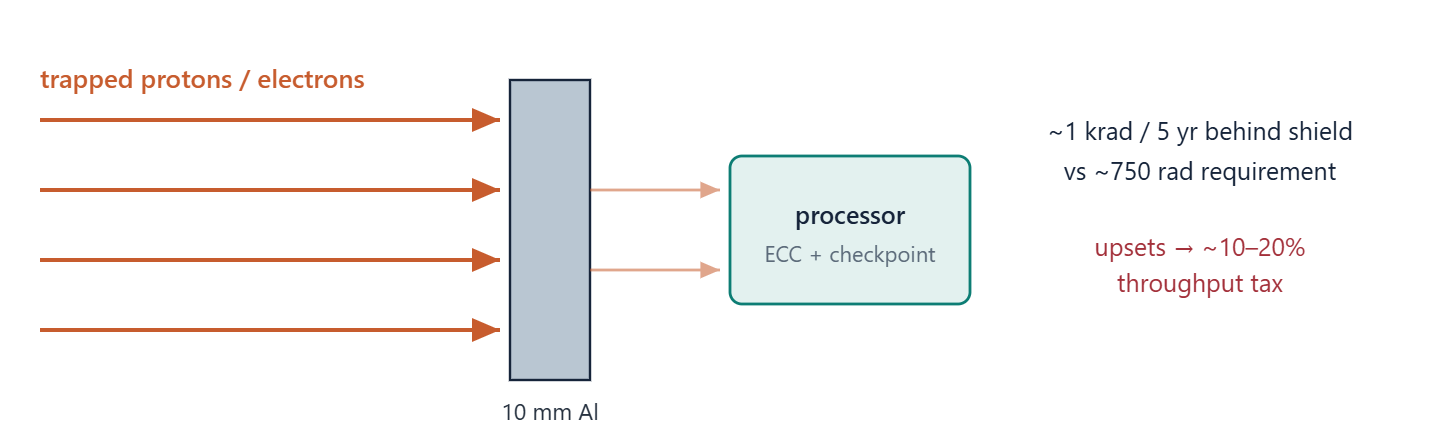
\includegraphics[keepaspectratio,alt={Radiation shielding and single-event upsets: aluminium attenuates the accumulated dose, while error correction and checkpointing handle upsets.}]{schematics/diagram_shield.png}}
\caption{Radiation shielding and single-event upsets: aluminium
attenuates the accumulated dose, while error correction and
checkpointing handle upsets.}
\end{figure}

\emph{Sources: trapped-particle fluxes from the AE8/AP8 {[}25{]} and
AE9/AP9 {[}26{]} models; dose-depth via SHIELDOSE {[}27{]}; environment
and effects from Tribble {[}22{]}, Pisacane {[}23{]}, and Hastings and
Garrett {[}24{]}.}

Two physically distinct radiation effects matter: the slow accumulation
of total ionizing dose, which is a shielding problem, and the stochastic
flipping of bits by energetic particles, which is a reliability and
throughput problem.

\textbf{Dose versus shielding.} Behind aluminium of thickness \(x\), the
trapped-electron contribution to dose attenuates quasi-exponentially
atop a floor set by penetrating protons and bremsstrahlung:

\begin{equation}
\dot D(x) = D_0\, e^{-x/\lambda} + D_\infty, \qquad \lambda \approx 1.7\ \mathrm{mm}. \tag{8.1}
\end{equation}

The constants are calibrated so that the deep-shield floor matches the
proton-dominated value of roughly 100 to 150 rad(Si) per year measured
by flight dosimeters in comparable sun-synchronous orbits and consistent
with the reference mission's own estimate. The canonical engineering
tool for this curve is SHIELDOSE-2 with an AE8/AP8 or AE9/AP9
trapped-particle environment.

\textbf{Result and margin.} At 10 mm of aluminium, the five-year
cumulative dose is approximately 1.06 krad(Si). The reference mission
reports that its processor's most sensitive subsystem, the
high-bandwidth memory, first showed irregularities at 2 krad(Si), about
three times the 750 rad(Si) five-year requirement, and exhibited no hard
failures up to the maximum tested dose of 15 krad(Si). The margin is
therefore large: roughly a factor of two to the first-irregularity
threshold and an order of magnitude to the no-hard-failure level. Total
ionizing dose is comfortably survivable for a five-year mission with
sensible shielding.

\begin{figure}
\centering
\pandocbounded{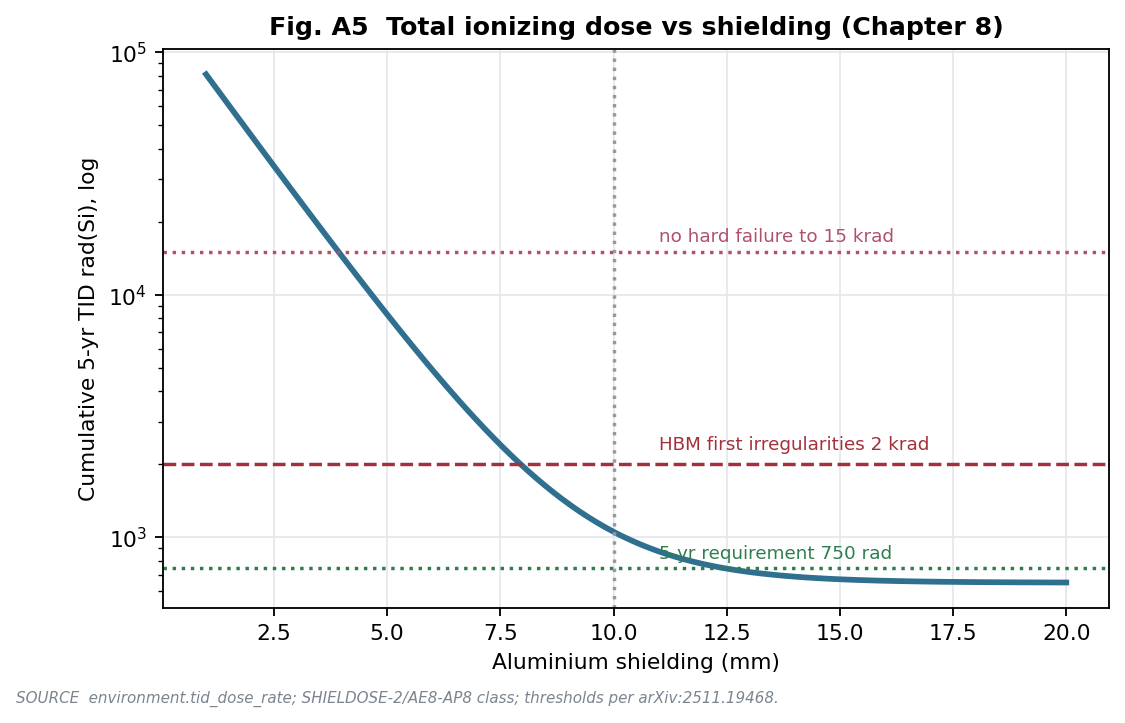
\includegraphics[keepaspectratio,alt={Fig. 8.1 Cumulative five-year ionizing dose versus aluminium shielding, with the memory tolerance and the mission requirement marked. Ten millimeters of aluminium keeps the dose well below the first-irregularity threshold.}]{figures2/figA5_dose.png}}
\caption{Fig. 8.1 Cumulative five-year ionizing dose versus aluminium
shielding, with the memory tolerance and the mission requirement marked.
Ten millimeters of aluminium keeps the dose well below the
first-irregularity threshold.}
\end{figure}

\textbf{Single-event effects.} Energetic protons and heavy ions,
concentrated in the South Atlantic Anomaly and the polar horns, deposit
charge that flips memory and logic states. The upset rate scales as
\(R_{\mathrm{SEU}} = \sigma_{\mathrm{SEU}}\,\phi\, N_{\mathrm{bits}}\),
the product of the per-bit cross-section, the particle flux, and the
number of bits. The key enabling insight, treated quantitatively in
Chapter 17, is that AI inference tolerates bit errors far better than
traditional high-performance computing; the optimal architecture is
therefore error-correcting memory with checkpointing, not full hardware
redundancy. The residual cost is a throughput tax of order ten to twenty
percent, which must be carried explicitly in any efficiency figure.

\textbf{Integrating the dose-depth law.} The cumulative dose quoted for
a fixed shielding thickness follows from integrating the dose rate of
Eq. (8.1) over the mission lifetime \(T\). Because the constants
\(D_0\), \(\lambda\), and \(D_\infty\) are taken as time-independent for
a stable orbit, the integral is elementary:

\begin{equation}
D(x,T) = \int_0^{T} \dot D(x)\, dt = \left( D_0\, e^{-x/\lambda} + D_\infty \right) T. \tag{8.2}
\end{equation}

The two terms separate cleanly into an electron component that the
shield attenuates and a floor that it does not. The shielding design
problem is to drive the first term below the second so that additional
aluminium yields diminishing returns. Setting the attenuated electron
term equal to a chosen fraction \(\epsilon\) of the floor gives the
thickness at which further mass is no longer productive:

\begin{equation}
x^{*} = \lambda \ln\!\left( \frac{D_0}{\epsilon\, D_\infty} \right). \tag{8.3}
\end{equation}

\textbf{Worked dose estimate.} The chapter states a five-year dose of
approximately 1.06 krad(Si) at \(x = 10\) mm. Treating the deep-shield
rate as dominated by the floor, the floor itself is recovered directly
from Eq. (8.2):

\begin{equation}
D_\infty \approx \frac{D(x,T)}{T} = \frac{1.06\ \mathrm{krad(Si)}}{5\ \mathrm{yr}} \approx 212\ \mathrm{rad(Si)\,yr^{-1}}, \tag{8.4}
\end{equation}

which sits in the same range as the 100 to 150 rad(Si) per year cited
for comparable sun-synchronous orbits once the small residual electron
term at 10 mm is included. The shielding margin is governed not by the
attenuation length, which is fixed by the spectrum, but by the floor, so
beyond roughly one to two centimetres of aluminium the design trades
shield mass for negligible dose reduction.

\textbf{Upset rate and the throughput tax.} Expanding the upset relation
\(R_{\mathrm{SEU}} = \sigma_{\mathrm{SEU}}\,\phi\, N_{\mathrm{bits}}\),
the fraction of operations corrupted per unit time is the upset rate
divided by the bit-access rate \(r_{\mathrm{acc}}\), and the throughput
tax \(\tau\) is the share of cycles reclaimed by error correction and
checkpoint replay:

\begin{equation}
\tau = \frac{c_{\mathrm{ECC}}\, R_{\mathrm{SEU}}}{r_{\mathrm{acc}}} = \frac{c_{\mathrm{ECC}}\, \sigma_{\mathrm{SEU}}\, \phi\, N_{\mathrm{bits}}}{r_{\mathrm{acc}}}, \tag{8.5}
\end{equation}

where \(c_{\mathrm{ECC}}\) is the average cycles charged per detected
upset. The tax scales linearly with flux, so it peaks in the South
Atlantic Anomaly and the polar horns and falls to a small floor
elsewhere, consistent with the bounded ten to twenty percent figure
carried in the efficiency budget.

\textbf{Design implication.} Shield to the dose floor rather than to an
arbitrary thickness, since mass past a centimetre or two buys almost no
margin; then size the compute overhead from Eq. (8.5) so that the upset
tax is budgeted explicitly rather than absorbed silently into throughput
claims.

\chapter{9. The Orbital-Debris
Environment}\label{the-orbital-debris-environment}

\begin{quote}
\emph{Abstract.} This chapter quantifies the debris hazard at the
reference altitude: the catastrophic-impact probability for the cluster
and the way a single fragmentation couples to neighbours as the spacing
tightens.
\end{quote}

\begin{figure}
\centering
\pandocbounded{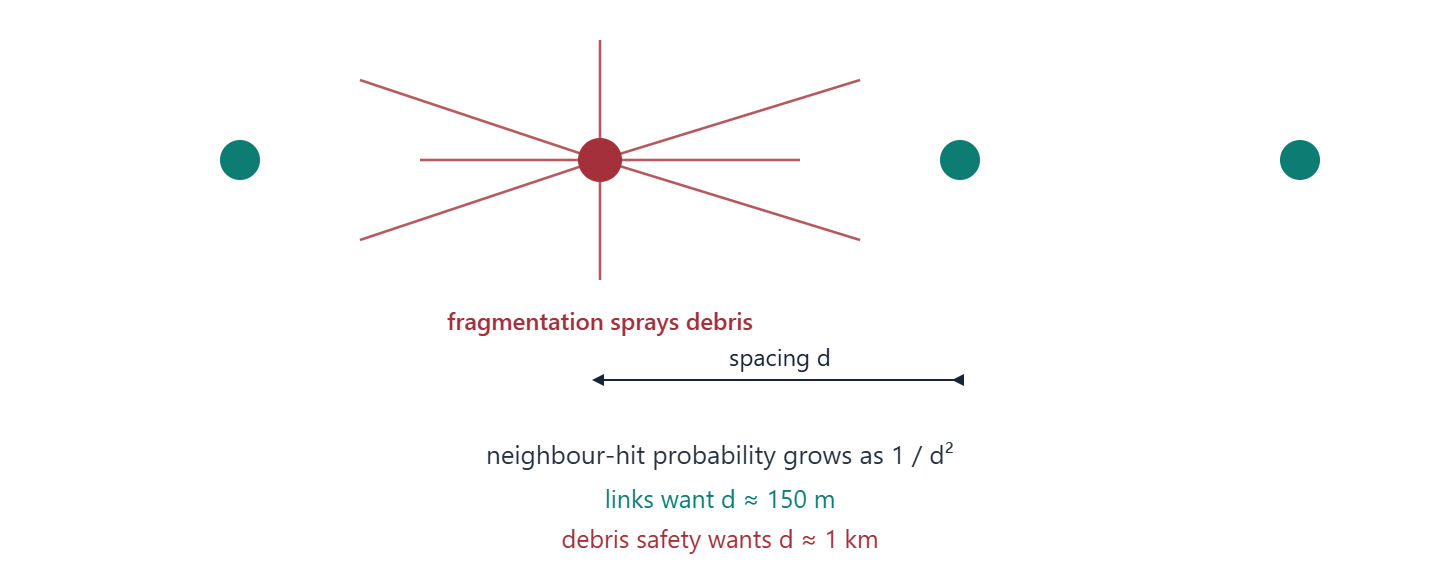
\includegraphics[keepaspectratio,alt={The formation paradox: one fragmentation sprays debris into the volume the neighbours occupy, with the neighbour-hit probability scaling as one over spacing squared.}]{schematics/diagram_formation.png}}
\caption{The formation paradox: one fragmentation sprays debris into the
volume the neighbours occupy, with the neighbour-hit probability scaling
as one over spacing squared.}
\end{figure}

\emph{Sources: flux from NASA ORDEM 3.2 {[}8{]} and ESA MASTER {[}9{]};
the collision-frequency and cascade framework follows Kessler and
Cour-Palais {[}28{]} and Klinkrad {[}29{]}.}

Low Earth orbit is increasingly congested, and the 650 km
sun-synchronous shell is among the most crowded. The European Space
Agency's environment models and NASA's ORDEM 3.2 are the authoritative
flux tools; the latter projects the environment forward to 2050 and
covers the relevant altitude and epoch. Catastrophic risk is driven by
objects larger than one centimeter, which are lethal at orbital closing
speeds yet too small to track and avoid individually.

\textbf{Impact probability as a Poisson process.} Impacts are rare,
independent events. Dividing a mission into \(n\) short intervals, each
with hit probability \(p = \Phi A\,\Delta t\) (flux times cross-section
times time), the number of impacts is binomial; in the limit
\(n\to\infty\) with \(np\to\Lambda\) it becomes Poisson with mean
\(\Lambda = \Phi A N t\), where \(N\) is the number of satellites. The
probability of at least one catastrophic impact in the cluster is

\begin{equation}
P(K \ge 1) = 1 - e^{-\Phi A N t}. \tag{9.1}
\end{equation}

With a model-class flux for objects larger than one centimeter of
\(\Phi = 3\times10^{-5}\
\mathrm{m^{-2}yr^{-1}}\), a tumbling-averaged silhouette of
\(A = 15\ \mathrm{m^2}\) per satellite, \(N = 81\), and \(t = 5\) years,
the mean is \(\Lambda = 0.182\) and the probability is about seventeen
percent, with a model band from six to forty-six percent. The
development of the cascade mechanism, the reason the tight formation is
dangerous, is given in Chapter 13 and the risk synthesis. The flux used
here is model-class; a flight program would run the official
ORDEM/MASTER tools for the exact orbit and epoch, as noted in Chapter
24.

\begin{center}\rule{0.5\linewidth}{0.5pt}\end{center}

\textbf{From the binomial limit to the Poisson mean.} The passage from
independent short intervals to a single closed-form probability deserves
the intermediate steps. Partition the mission into \(n\) equal slices of
duration \(\Delta t = t/n\). If \(p = \Phi A\,\Delta t\) is the
per-slice, per-satellite hit probability, the count of catastrophic
impacts across \(N\) satellites and \(n\) slices follows a binomial law
with trial number \(m = Nn\) and success probability \(p\). The
probability of zero impacts is

\begin{equation}
P(K = 0) = (1 - p)^{m} = \left(1 - \frac{\Phi A N t}{m}\right)^{m}. \tag{9.2}
\end{equation}

Taking the limit \(m \to \infty\) at fixed product \(mp = \Phi A N t\),
and using \(\lim_{m\to\infty}(1 - x/m)^{m} = e^{-x}\), the zero-impact
probability collapses to \(e^{-\Phi A N t}\). The complement is the
at-least-one expression already stated as Equation (9.1); the grouped
mean is

\begin{equation}
\Lambda = m p = \Phi A N t, \tag{9.3}
\end{equation}

which makes explicit that the hazard scales linearly in flux,
silhouette, fleet size, and mission length. This linearity is the reason
a long-lived, many-node cluster cannot escape the environment by clever
scheduling; only the four factors in Equation (9.3) move the risk.

\textbf{Worked mean and the small-\(\Lambda\) reading.} Substituting the
chapter's reference values,
\(\Phi = 3\times10^{-5}\ \mathrm{m^{-2}yr^{-1}}\),
\(A = 15\ \mathrm{m^2}\), \(N = 81\), and \(t = 5\ \mathrm{yr}\), gives

\begin{equation}
\Lambda = (3\times10^{-5})(15)(81)(5) = 0.182, \tag{9.4}
\end{equation}

in agreement with the value quoted in the text. Because \(\Lambda\) is
below unity, the series expansion
\(1 - e^{-\Lambda} = \Lambda - \Lambda^2/2 + \cdots\) shows that
\(P(K\ge 1)\) sits slightly under \(\Lambda\) itself, here near
seventeen percent, while the expected number of distinct impacts is just
\(\Lambda\). The two coincide only to first order, so reporting the mean
and the probability separately is appropriate.

\textbf{Per-satellite versus fleet risk.} It is often useful to separate
the single-vehicle exposure from the aggregate. Writing
\(\lambda_1 = \Phi A t\) for one satellite, the fleet survival
probability is the product of independent survivals,

\begin{equation}
P(K = 0) = \left(e^{-\lambda_1}\right)^{N} = e^{-N\lambda_1}, \tag{9.5}
\end{equation}

which recovers Equation (9.1) and confirms the independence assumption
is what permits the simple exponent \(N\lambda_1\). The design
implication is direct: since fleet risk grows as the product
\(N\lambda_1\), halving the tumbling-averaged silhouette \(A\) buys the
same risk reduction as halving either the node count or the mission
duration.

\part{SPACECRAFT SUBSYSTEMS}\label{spacecraft-subsystems}

\chapter{10. Thermal Control}\label{thermal-control}

\begin{quote}
\emph{Abstract.} This chapter develops the thermal model, the linear
scaling of radiator area with power and the sharper wall at the chip
interface, and identifies the power level above which a passive path can
no longer cope.
\end{quote}

\begin{figure}
\centering
\pandocbounded{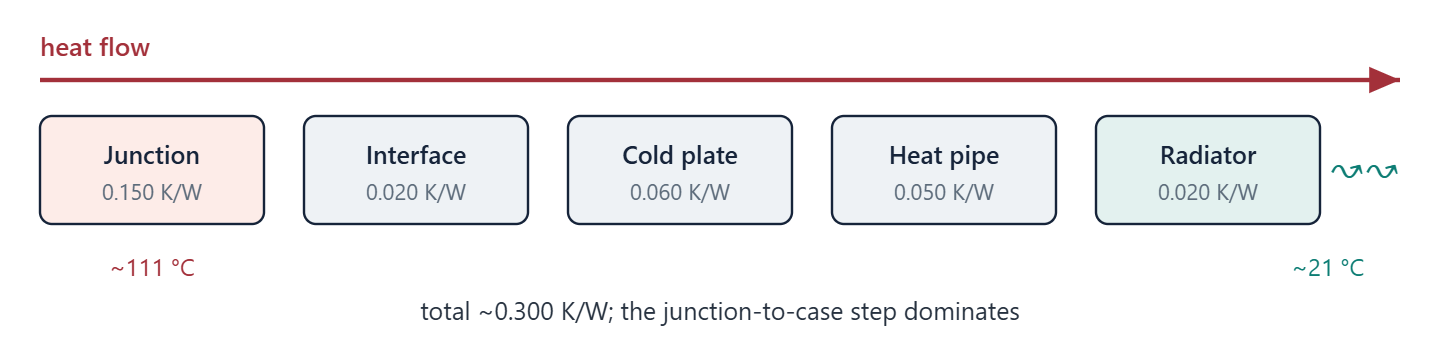
\includegraphics[keepaspectratio,alt={The passive conduction path from the junction to the radiator, dominated by the junction-to-case resistance.}]{schematics/diagram_thermal.png}}
\caption{The passive conduction path from the junction to the radiator,
dominated by the junction-to-case resistance.}
\end{figure}

\emph{Sources: radiative and conductive relations from Incropera and
DeWitt {[}21{]}; spacecraft-specific practice from the Gilmore
thermal-control handbook {[}20{]} and ECSS-E-ST-31C {[}34{]}.}

Thermal control is where the orbital data center is most often assumed
to be hard and is in fact solved at the single-node scale, but it does
not scale for free, and a second, sharper limit appears at the chip
interface.

\textbf{From Planck's law to Stefan-Boltzmann.} A blackbody emits
spectral radiance

\begin{equation}
B(\lambda, T) = \frac{2 h_P c^2}{\lambda^5}\,\frac{1}{\exp(h_P c / \lambda k_B T) - 1}. \tag{10.1}
\end{equation}

Integrating over the emitting hemisphere (the factor \(\pi\) from
\(\int\cos\theta\,d\Omega\)) and over all wavelengths gives the
hemispherical emissive power,

\begin{equation}
E_b(T) = \pi\!\int_0^\infty B(\lambda, T)\,d\lambda = \sigma T^4, \qquad
\sigma = \frac{2\pi^5 k_B^4}{15 h_P^3 c^2}. \tag{10.2}
\end{equation}

A gray surface of emissivity \(\varepsilon\) radiating to the
cosmic-microwave-background sink at \(T_{\mathrm{CMB}}\) rejects
\(Q_{\mathrm{rad}} = \varepsilon\sigma A (T^4 - T_{\mathrm{CMB}}^4)\);
since \(T_{\mathrm{CMB}}^4/T^4 \sim 10^{-8}\) at room temperature, the
sink term is negligible.

\textbf{Radiator sizing.} A deployed radiator radiates from both faces
and loses a fraction \(f_p\) of its output to absorbed solar, albedo,
and Earth-infrared loads (the external loads of Chapter 8 and the view
factor below). The net rejected flux per unit one-side area is
\(\varepsilon\sigma T^4 n_s (1-f_p)\) with \(n_s = 2\), so the required
area for a heat load \(Q\) at operating temperature \(T\) is

\begin{equation}
A_{\mathrm{rad}} = \frac{Q}{\varepsilon\,\sigma\,T^4\,n_s\,(1 - f_p)}. \tag{10.3}
\end{equation}

This is \textbf{linear in \(Q\)}: there is no economy of scale in
radiative cooling, a fact with profound architectural consequences.
\textbf{Worked example:} at 1 MW, 20 C, \(\varepsilon = 0.90\),
\(n_s = 2\), \(f_p = 0.12\), the per-side flux is
\(\varepsilon\sigma T^4 = 376.9\ \mathrm{W/m^2}\), the net flux is
\(663.3\ \mathrm{W/m^2}\), and
\(A_{\mathrm{rad}} = 1508\ \mathrm{m^2}\). This matches the industry
rule of roughly 1,200 m² per megawatt and explains why Starcloud's
gigawatt vision implies multi-kilometer panels.

\begin{figure}
\centering
\pandocbounded{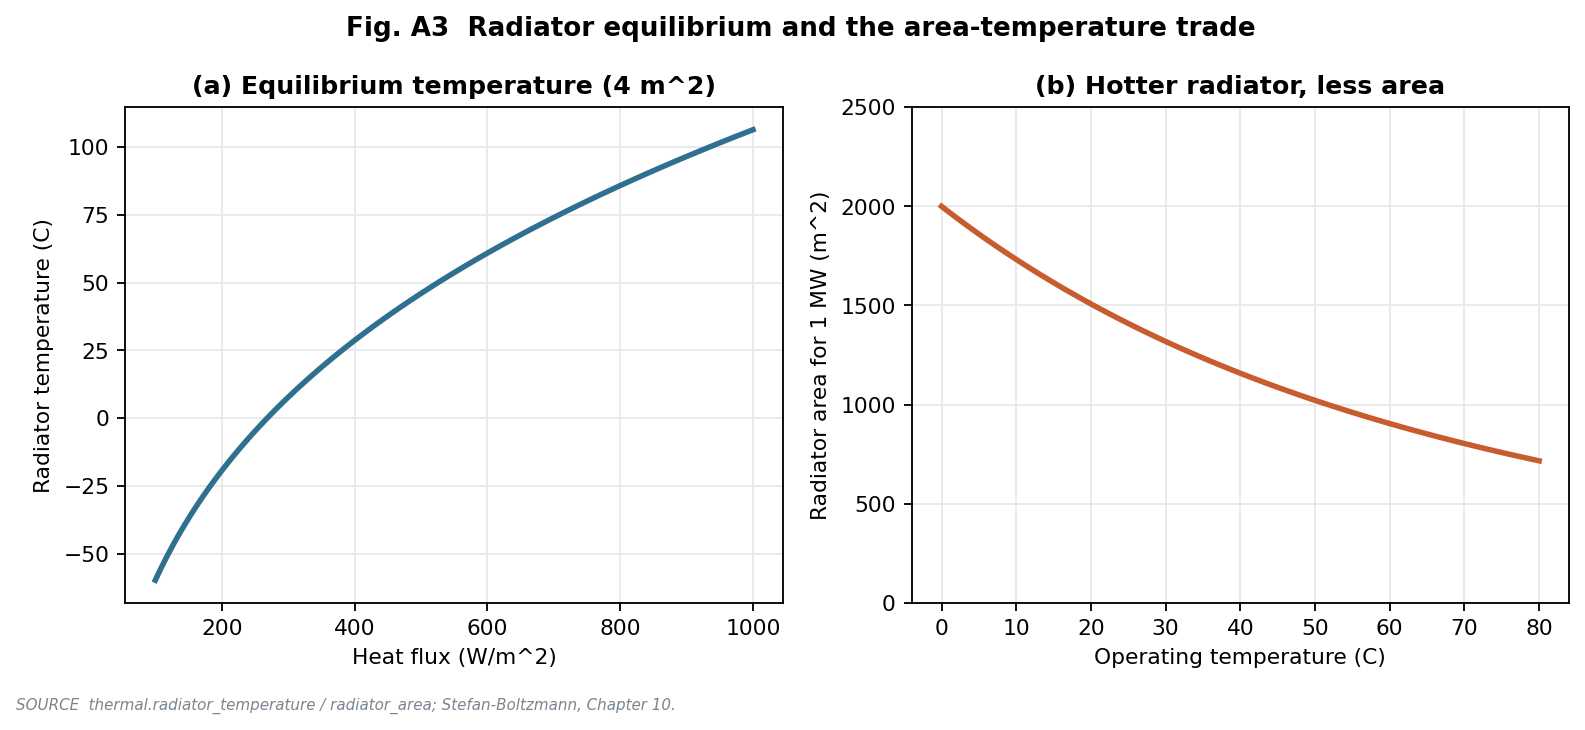
\includegraphics[keepaspectratio,alt={Fig. 10.1 Radiator equilibrium temperature versus heat flux, and the radiator area required for one megawatt versus operating temperature. Running hotter reduces area at the cost of silicon lifetime.}]{figures2/figA3_radiator.png}}
\caption{Fig. 10.1 Radiator equilibrium temperature versus heat flux,
and the radiator area required for one megawatt versus operating
temperature. Running hotter reduces area at the cost of silicon
lifetime.}
\end{figure}

\textbf{External loads and view factor.} A surface at orbital radius
\(r\) sees Earth through the view factor
\(F = \tfrac{1}{2}[1 - \sqrt{1 - (R_E/r)^2}]\), equal to 0.290 at 650
km. The absorbed loads are
\(Q_{\mathrm{albedo}} = S_0\, a_{\mathrm{alb}}\, F\, \alpha_s\, A\) and
\(Q_{\mathrm{IR}} =
q_{\mathrm{IR}}\, F\, \varepsilon\, A\); for an edge-on radiator the
direct-solar term vanishes. With \(\alpha_s = 0.15\) and
\(A = 4\ \mathrm{m^2}\) these are about 71 W and 251 W respectively,
which the design lumps to roughly 100 W of parasitic load.

\begin{figure}
\centering
\pandocbounded{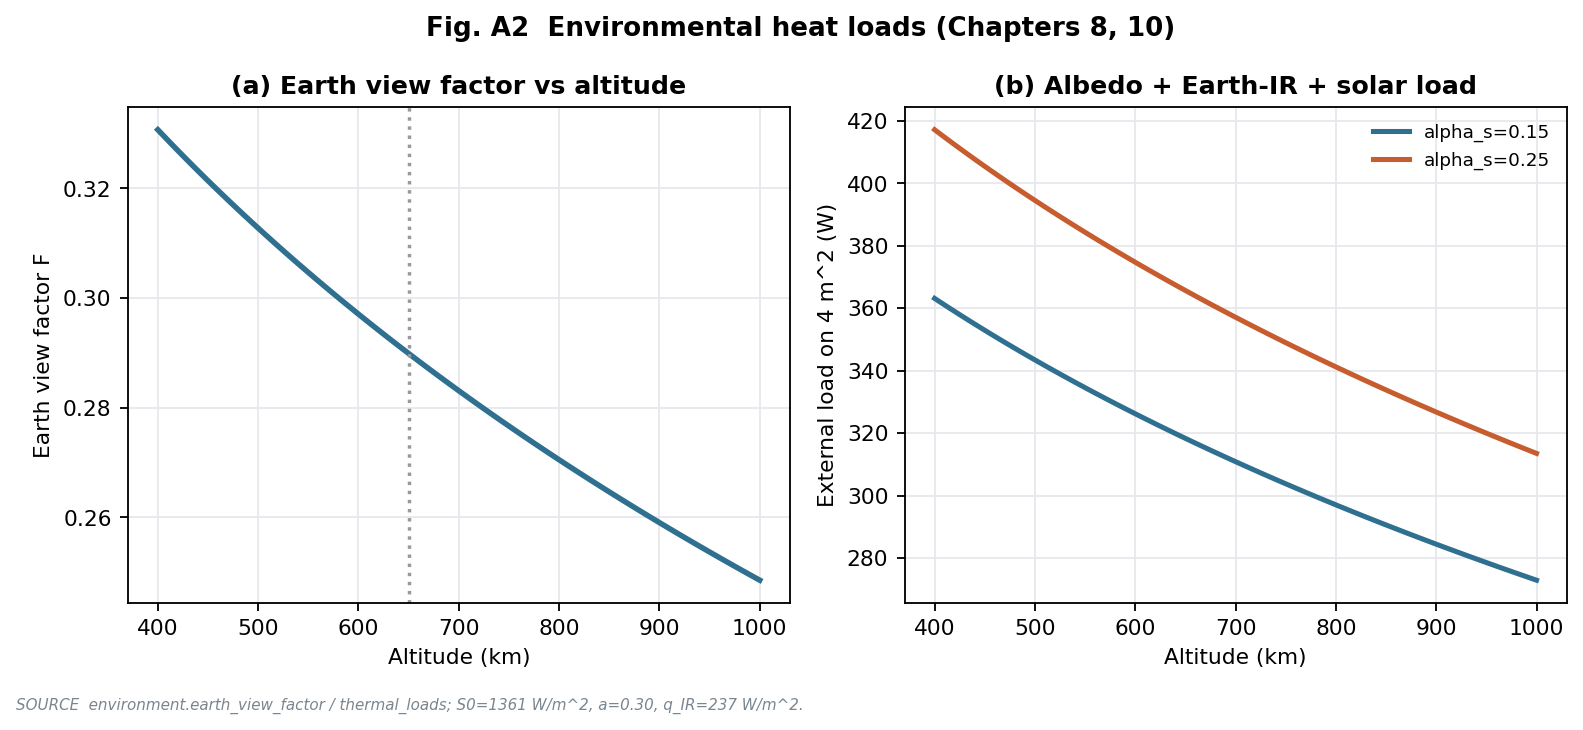
\includegraphics[keepaspectratio,alt={Fig. 10.2 Earth view factor versus altitude, and the combined albedo, Earth-infrared, and solar load on a four-square-meter surface. External loads set the parasitic fraction in the radiator sizing.}]{figures2/figA2_loads.png}}
\caption{Fig. 10.2 Earth view factor versus altitude, and the combined
albedo, Earth-infrared, and solar load on a four-square-meter surface.
External loads set the parasitic fraction in the radiator sizing.}
\end{figure}

\textbf{Inverse problem and Newton-Raphson.} When the area is fixed and
the temperature is sought, (10.3) becomes a quartic, solved by
Newton-Raphson on \(f(T) = Q - \varepsilon\sigma A T^4\) with
\(f'(T) = -4\varepsilon\sigma A T^3\), converging in two to four
iterations from \(T_0 = 300\) K. The first report's baseline (1450 W on
4 m², \(\varepsilon = 0.85\), single-sided) yields a radiator
temperature of 21.4 C.

\textbf{The conductive chain and the interface wall.} Heat first travels
from the junction to the radiator through series resistances,
\(T_j = T_{\mathrm{rad}} + Q\, R_{th}\). With the passive chain
\(R_{th} = 0.30\ \mathrm{K/W}\), the rise across the interface alone is
\(P \times 0.30\): 90 C at 300 W, \textbf{210 C at 700 W, and 360 C at
1200 W}. Because the entire junction budget is 125 C, any chip with
\(P\, R_{th} > 125\ \mathrm{C}\), that is, \(P > 417\ \mathrm{W}\),
cannot be cooled passively at any radiator size. Above this threshold,
chip-level liquid or loop-heat-pipe cooling is mandatory. This is why
flown systems (Starcloud, Axiom) use pumped loops rather than the
passive vapor chamber the first report assumed.

\begin{figure}
\centering
\pandocbounded{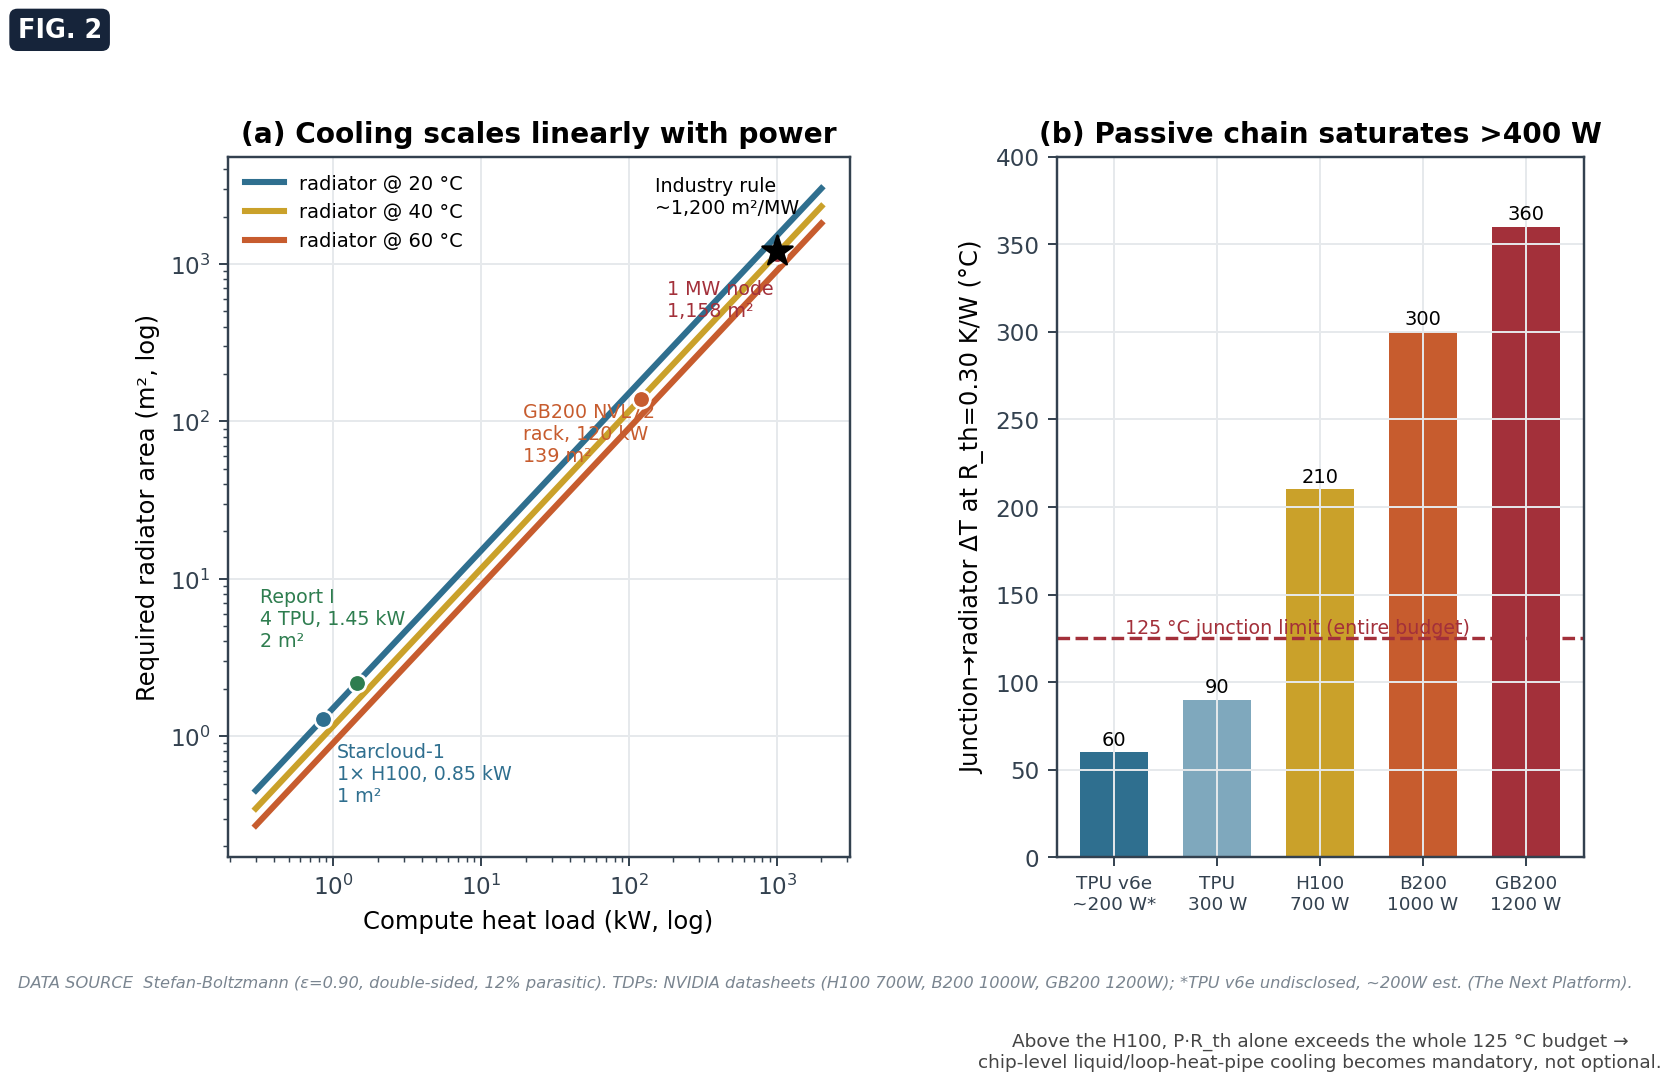
\includegraphics[keepaspectratio,alt={Fig. 10.1, (a) Radiator area is linear in heat load; (b) the passive thermal chain saturates above \textasciitilde400 W, forcing chip-level active cooling.}]{figures/fig2_thermal_wall.png}}
\caption{Fig. 10.1, (a) Radiator area is linear in heat load; (b) the
passive thermal chain saturates above \textasciitilde400 W, forcing
chip-level active cooling.}
\end{figure}

\textbf{Deriving the radiator scaling from the energy balance.} The
sizing relation (10.3) follows from a steady-state energy balance on the
panel. In equilibrium the dissipated electrical load \(Q\) equals the
net radiated power, while the absorbed external loads of Chapter 8
reduce the useful output by the fraction \(f_p\). Writing the balance
for a two-sided panel of one-side area \(A_{\mathrm{rad}}\),

\begin{equation}
Q = \varepsilon\,\sigma\,n_s\,A_{\mathrm{rad}}\,(T^4 - T_{\mathrm{CMB}}^4)\,(1 - f_p). \tag{10.4}
\end{equation}

Dropping the sink term, since \(T_{\mathrm{CMB}}^4/T^4 \sim 10^{-8}\),
and solving for the area returns (10.3) exactly. The linearity in \(Q\)
is therefore structural, not incidental; the area carries no exponent
that would let a larger plant reject heat more cheaply per watt.

\textbf{Sensitivity to operating temperature.} Because the rejected flux
varies as \(T^4\), the marginal benefit of running the silicon hotter is
large. Differentiating (10.3) at fixed \(Q\), \(\varepsilon\), \(n_s\),
and \(f_p\),

\begin{equation}
\frac{dA_{\mathrm{rad}}}{A_{\mathrm{rad}}} = -4\,\frac{dT}{T}. \tag{10.5}
\end{equation}

A one percent rise in absolute operating temperature reduces the
required area by about four percent. This is the quantitative form of
the trade noted in Fig. 10.1: area is bought back by raising \(T\), at
the cost of junction lifetime.

\textbf{The conductive chain and the passive ceiling.} The series
resistance model \(T_j = T_{\mathrm{rad}} + Q\,R_{th}\) sets the second
limit. Requiring the junction to stay within its allowable rise
\(\Delta T_{\max} = T_{j,\max} - T_{\mathrm{rad}}\) bounds the power a
passive chain can carry,

\begin{equation}
P_{\max} = \frac{\Delta T_{\max}}{R_{th}}. \tag{10.6}
\end{equation}

\textbf{Worked example.} Taking the chapter's junction budget
\(\Delta T_{\max} = 125\ \mathrm{C}\) and the passive chain
\(R_{th} = 0.30\ \mathrm{K/W}\),

\begin{equation}
P_{\max} = \frac{125\ \mathrm{C}}{0.30\ \mathrm{K/W}} \approx 417\ \mathrm{W}. \tag{10.7}
\end{equation}

This reproduces the 417 W threshold and confirms that no radiator size
relaxes it, since \(R_{th}\) acts before the heat reaches the panel.

\textbf{Design implication.} Radiator mass scales linearly with plant
power and the chip interface caps any single device near 417 W
passively; an orbital data center must therefore plan for
kilometer-scale panels and adopt pumped-loop or loop-heat-pipe cooling
at the chip from the outset.

\chapter{11. Electrical Power}\label{electrical-power}

\begin{quote}
\emph{Abstract.} This chapter sizes the electrical-power subsystem for
the dawn-dusk orbit, where near-continuous sunlight makes the battery
small and the array sizing the dominant term.
\end{quote}

\emph{Sources: solar-array and power-budget sizing from SMAD {[}18{]}
and the Gilmore handbook {[}20{]}; cell and battery parameters from
vendor datasheets {[}12{]}.}

The power subsystem converts sunlight to usable electrical power and
buffers the brief eclipse.

\textbf{Array power.} The electrical power delivered to the load is the
incident solar power times the cell efficiency (which falls with
temperature and degrades with radiation), the panel packing factor, and
the array-to-load path efficiency:

\begin{equation}
P = S_0\, A\, \eta(T,\mathrm{life})\, \kappa_{\mathrm{pack}}\, \eta_{\mathrm{path}}, \qquad
\eta(T,\mathrm{life}) = \eta_{\mathrm{life}}\,\big[1 + k_T (T - 28)\big]. \tag{11.1}
\end{equation}

Triple-junction GaInP/GaAs/Ge cells deliver about 29.6 percent at
beginning of life and 27.5 percent after a five-year fluence, with a
temperature coefficient \(k_T \approx -0.0023\ \mathrm{per\ C}\),
packing \(\kappa_{\mathrm{pack}} = 0.85\), and path efficiency
\(\eta_{\mathrm{path}} = 0.88\). \textbf{Worked example:} at end of life
and 70 C, \(\eta = 0.275[1 - 0.0023(70-28)] = 0.248\), so
\(P = 1361 \times 1 \times 0.248 \times 0.85 \times 0.88 = 253\ \mathrm{W/m^2}\)
at the load.

\textbf{Battery and the dawn-dusk lever.} To carry the load \(P_L\)
through an eclipse of duration \(t_e\) at depth-of-discharge DoD and
specific energy \(e_{\mathrm{sp}}\), the battery mass is
\(m_{\mathrm{bat}} = P_L t_e / (\mathrm{DoD}\, e_{\mathrm{sp}})\). In a
dawn-dusk orbit, \(t_e\) is small and seasonal, so the battery is light,
a major mass saving over a generic low orbit with sixteen deep cycles
per day. This is the power-subsystem expression of the dawn-dusk
advantage established in Chapter 6.

\begin{figure}
\centering
\pandocbounded{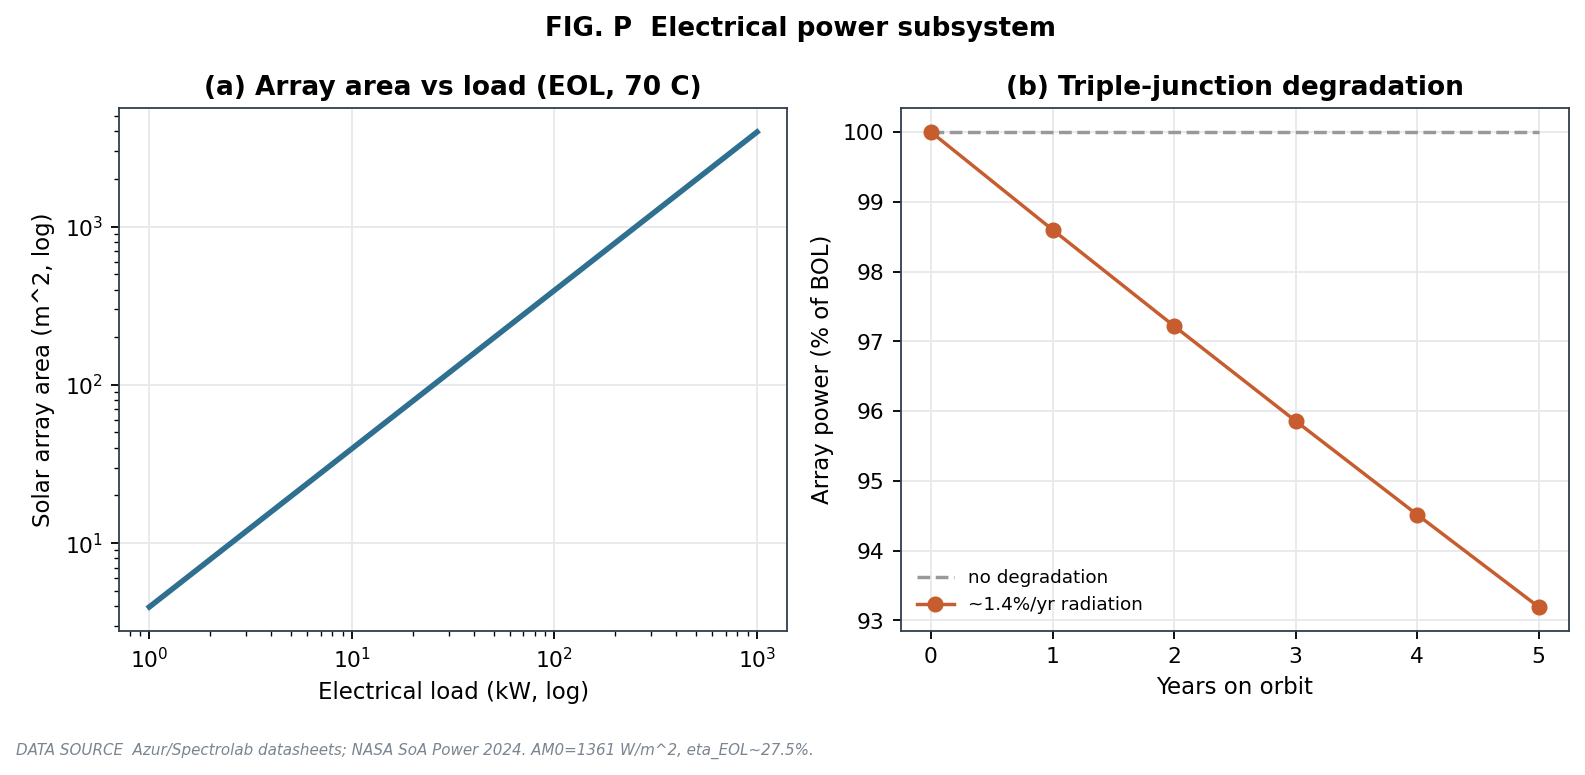
\includegraphics[keepaspectratio,alt={Fig. 11.1, Array area versus load, and triple-junction degradation over the mission.}]{systems_figs/fig_power.png}}
\caption{Fig. 11.1, Array area versus load, and triple-junction
degradation over the mission.}
\end{figure}

\textbf{Deriving the temperature-and-life efficiency factor.} The cell
efficiency in equation (11.1) combines two independent degradation
paths, and it is worth separating them. The radiation-driven fall from
beginning-of-life efficiency \(\eta_{\mathrm{BOL}}\) to the end-of-life
value \(\eta_{\mathrm{life}}\) is multiplicative over the mission, so
for an annual degradation rate \(d\) acting over \(N\) years the
surviving fraction is

\begin{equation}
\eta_{\mathrm{life}} = \eta_{\mathrm{BOL}}\,(1 - d)^{N}. \tag{11.2}
\end{equation}

Linearizing the temperature term about the reference temperature of 28
C, the relative efficiency change is the temperature coefficient times
the excursion, which recovers the bracketed factor of (11.1):

\begin{equation}
\frac{\eta(T) - \eta_{\mathrm{life}}}{\eta_{\mathrm{life}}} = k_T\,(T - 28). \tag{11.3}
\end{equation}

Using \(\eta_{\mathrm{BOL}} = 0.296\) and
\(\eta_{\mathrm{life}} = 0.275\) over five years, equation (11.2) gives
an implied annual rate \(d = 1 - (0.275/0.296)^{1/5} \approx 0.0147\),
that is about 1.5 percent per year, consistent with the five-year
fluence quoted for the triple-junction cell.

\textbf{Array equilibrium temperature.} Because \(\eta\) depends on
\(T\), the operating temperature is itself set by a radiative balance
and should be solved, not assumed. Equating absorbed solar flux to
emitted thermal flux from both faces of the panel, with absorptance
\(\alpha\), front and back emittances \(\varepsilon_f + \varepsilon_b\),
and the electrical power drawn off the front face, gives

\begin{equation}
\alpha\,S_0 = (\varepsilon_f + \varepsilon_b)\,\sigma\,T^4 + S_0\,\eta\,\kappa_{\mathrm{pack}}, \tag{11.4}
\end{equation}

so that, solving for the equilibrium temperature,

\begin{equation}
T = \left[\frac{S_0\,(\alpha - \eta\,\kappa_{\mathrm{pack}})}{(\varepsilon_f + \varepsilon_b)\,\sigma}\right]^{1/4}. \tag{11.5}
\end{equation}

Equations (11.5) and (11.3) form a small fixed point: a hotter panel
lowers \(\eta\), which in turn raises the equilibrium temperature
slightly. One or two iterations from the 70 C operating point used in
the worked example of (11.1) are sufficient for sizing.

\textbf{Array sizing closure.} Inverting the load relation of (11.1)
gives the collecting area required to meet a load \(P_L\),

\begin{equation}
A = \frac{P_L}{S_0\,\eta(T,\mathrm{life})\,\kappa_{\mathrm{pack}}\,\eta_{\mathrm{path}}}, \tag{11.6}
\end{equation}

which at the end-of-life value of \(253\ \mathrm{W/m^2}\) delivered to
the load means each megawatt of demand needs roughly
\(3953\ \mathrm{m^2}\) of array.

\textbf{Design implication.} Because the array area scales inversely
with the temperature-depressed end-of-life efficiency, the panel thermal
design and the radiation-tolerant cell selection are leveraged directly
into deployed area and structural mass; cooling or de-rating the array
is a sizing decision, not a comfort margin.

\chapter{12. Structures and Mass}\label{structures-and-mass}

\begin{quote}
\emph{Abstract.} This chapter estimates the structural and mass
properties, the inertia tensor, the structural mass set by launch loads,
and the panel modal frequency, that feed the attitude and integration
analyses.
\end{quote}

\emph{Sources: mass-growth allowances from AIAA S-120 {[}14{]};
structural and modal relations from SMAD {[}18{]} and Sidi {[}33{]}.}

The structure carries launch loads, sets the spacecraft inertia (which
feeds attitude control), and anchors the mass budget that closes the
whole design.

\textbf{Inertia from geometry.} A uniform box of mass \(m\) and
dimensions \(d_x, d_y, d_z\) has principal moments
\(I_x = \tfrac{m}{12}(d_y^2 + d_z^2)\), and cyclic permutations. A
deployed panel of mass \(m\), length \(L\), at offset \(o\) from the bus
axis contributes \(m(L^2/12 + o^2)\) by the parallel-axis theorem.
Summing the bus, two solar wings, and the radiators gives a diagonal
inertia tensor; for the reference satellite the maximum principal moment
is on the order of a few hundred kilogram-meters squared, and the
maximum minus minimum difference feeds the gravity-gradient torque of
Chapter 13.

\textbf{Structural mass and launch loads.} Primary structure is sized as
a fraction (typically fifteen to twenty-five percent) of the supported
mass, and checked against the quasi-static launch load: the stress in a
primary member is
\(\sigma_{\mathrm{stress}} = m\, g_{\mathrm{load}}\, g_0 / A_{\mathrm{member}}\),
and the margin is the yield strength divided by this stress, required to
exceed roughly 1.25 with margin. For aluminium at an 8.5-g quasi-static
load, modest member areas keep the margin comfortable.

\textbf{Panel fundamental frequency.} Deployed panels must be stiff
enough that their fundamental mode does not couple to the
attitude-control bandwidth. For a plate of side \(a\), thickness \(t\),
and areal mass \(\rho_A\),

\begin{equation}
f_1 = \frac{\beta}{2\pi}\sqrt{\frac{D}{\rho_A\, a^4}}, \qquad D = \frac{E t^3}{12(1-\nu^2)}, \tag{12.1}
\end{equation}

with \(\beta\) a boundary-condition constant. Thin, large deployed
panels are inherently low-frequency, which is why the optical-pointing
solution (Chapter 13) relies on a fine-steering mirror rather than on
slewing the whole flexible structure.

\textbf{Mass closure.} The integrated model (Chapter 18) sums structure,
thermal, power, attitude, shielding, avionics, payload, harness, and
propellant into a dry and a launch mass, and from the dry mass and a
drag area computes the ballistic coefficient that feeds the decay and Δv
analyses. The reference four-chip satellite closes at roughly 270 to 290
kg dry.

\begin{figure}
\centering
\pandocbounded{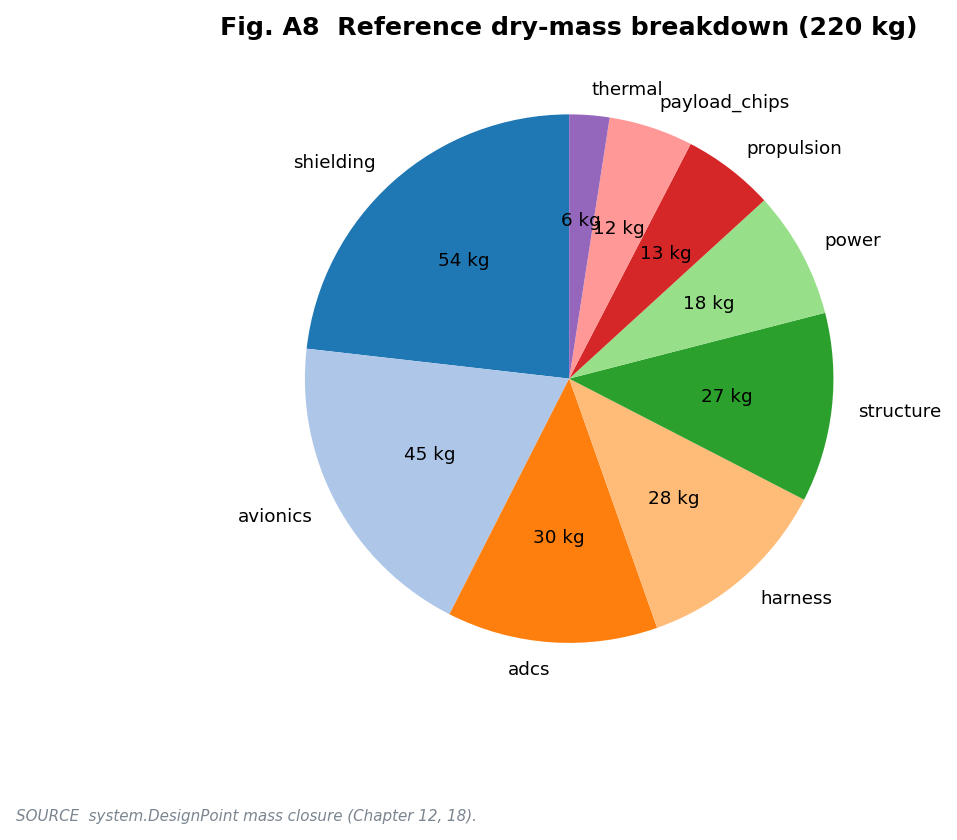
\includegraphics[keepaspectratio,alt={Fig. 12.1 Reference satellite dry-mass breakdown by subsystem, closed self-consistently by the integrated model.}]{figures2/figA8_mass.png}}
\caption{Fig. 12.1 Reference satellite dry-mass breakdown by subsystem,
closed self-consistently by the integrated model.}
\end{figure}

\textbf{Derivation of the box inertia.} The principal moment of a
uniform rectangular solid follows from integrating the mass element over
the body. For rotation about the \(x\) axis the relevant distance from
the axis is \(r^2 = y^2 + z^2\), so with uniform density
\(\rho = m/(d_x d_y d_z)\),

\begin{equation}
I_x = \int_V (y^2 + z^2)\,\rho\,dV = \rho \int_{-d_x/2}^{d_x/2}\!\!\int_{-d_y/2}^{d_y/2}\!\!\int_{-d_z/2}^{d_z/2} (y^2 + z^2)\,dz\,dy\,dx. \tag{12.2}
\end{equation}

Each quadratic integral over a span \(d\) centred on the origin yields
\(\int_{-d/2}^{d/2} y^2\,dy = d^3/12\). Carrying the three integrations
and grouping the surviving factors gives

\begin{equation}
I_x = \rho\, d_x \left( \frac{d_y^3}{12} d_z + d_y \frac{d_z^3}{12} \right) = \frac{m}{12}\left(d_y^2 + d_z^2\right), \tag{12.3}
\end{equation}

which is the chapter's stated result, with the \(y\) and \(z\) moments
following by cyclic permutation.

\textbf{Parallel-axis contribution of an offset panel.} A panel of mass
\(m\) has a moment \(I_{\mathrm{cm}} = mL^2/12\) about its own
centroidal axis. Translating that axis a distance \(o\) to the bus axis
adds the point-mass term \(m o^2\), so

\begin{equation}
I_{\mathrm{panel}} = I_{\mathrm{cm}} + m o^2 = m\left(\frac{L^2}{12} + o^2\right), \tag{12.4}
\end{equation}

confirming the relation used to assemble the diagonal tensor from bus,
wings, and radiators.

\textbf{Worked launch-load check.} Take a single primary member of area
\(A_{\mathrm{member}}\) supporting a tributary mass \(m\) at the
quasi-static load \(g_{\mathrm{load}} = 8.5\) stated in the chapter. The
member stress is
\(\sigma_{\mathrm{stress}} = m\,g_{\mathrm{load}}\,g_0 / A_{\mathrm{member}}\),
and the strength margin against a yield strength \(\sigma_y\) is

\begin{equation}
\mathrm{MS} = \frac{\sigma_y}{F_s\,\sigma_{\mathrm{stress}}} - 1 = \frac{\sigma_y\, A_{\mathrm{member}}}{F_s\, m\, g_{\mathrm{load}}\, g_0} - 1, \tag{12.5}
\end{equation}

where \(F_s\) is the factor of safety. Setting \(\mathrm{MS} = 0\)
inverts to the minimum member area,

\begin{equation}
A_{\mathrm{member,\,min}} = \frac{F_s\, m\, g_{\mathrm{load}}\, g_0}{\sigma_y}, \tag{12.6}
\end{equation}

so the required cross-section scales linearly with supported mass and
load factor and inversely with material strength.

\textbf{Design implication.} Because inertia grows with the square of
panel length and offset while the launch-driven member area grows only
linearly with mass, large deployed structures are dominated by their
inertial and modal penalties rather than by static strength; the mass
budget should therefore be tightened at the geometry stage, before
member sizing.

\chapter{13. Attitude Determination and Control; Optical
Pointing}\label{attitude-determination-and-control-optical-pointing}

\begin{quote}
\emph{Abstract.} This chapter treats attitude determination and control
and the much finer pointing the optical links demand, showing why a
fast-steering mirror is required on top of the spacecraft bus.
\end{quote}

\begin{figure}
\centering
\pandocbounded{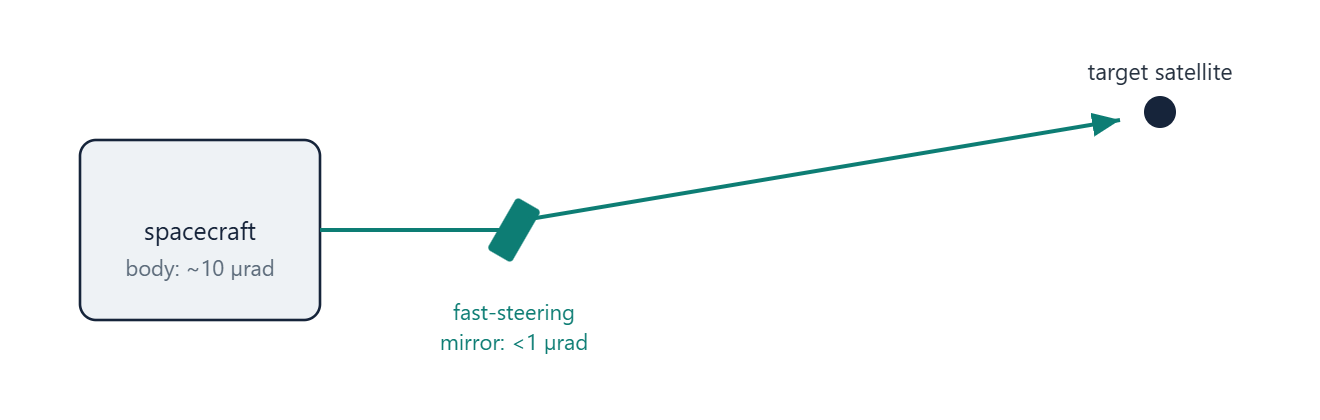
\includegraphics[keepaspectratio,alt={Coarse body pointing combined with a fast-steering mirror, which supplies the sub-microradian correction the optical link requires.}]{schematics/diagram_pointing.png}}
\caption{Coarse body pointing combined with a fast-steering mirror,
which supplies the sub-microradian correction the optical link
requires.}
\end{figure}

\emph{Sources: attitude dynamics and control from Wertz {[}32{]} and
Sidi {[}33{]}; optical-pointing requirements from Hemmati {[}30{]}.}

The attitude subsystem must hold the bus steady against disturbance
torques and, far more demandingly, point laser links to sub-microradian
accuracy.

\textbf{Disturbance torques.} The dominant low-orbit torques are
gravity-gradient and aerodynamic:

\begin{equation}
\tau_{\mathrm{gg}} = \tfrac{3}{2}\, n^2\, |I_z - I_x|\, \sin 2\theta, \qquad
\tau_{\mathrm{aero}} = \tfrac{1}{2}\rho v^2 C_D A\,\ell_{cp\text{-}cg}, \tag{13.1}
\end{equation}

where \(\ell_{cp\text{-}cg}\) is the offset between the center of
pressure and the center of mass. With the geometry-derived inertia of
Chapter 12, the gravity-gradient torque at 650 km is of order
\(10^{-4}\ \mathrm{N\,m}\). Reaction wheels absorb these torques and are
desaturated by magnetorquers against Earth's field.

\textbf{Optical pointing and the fine-steering mirror.} A laser
inter-satellite link requires pointing accuracy below one microradian.
The diffraction-limited beam divergence is \(\Theta \approx 2.44\,
\lambda/D\), and a pointing error \(\theta_{\mathrm{err}}\) relative to
the beam divergence \(\theta_{\mathrm{div}}\) costs received power
\(L_{\mathrm{point}} = \exp(-2\theta_{\mathrm{err}}^2/
\theta_{\mathrm{div}}^2)\). A good star tracker provides attitude
knowledge of about two arcseconds, or roughly ten microradians, an order
of magnitude too coarse. The bus alone cannot hold the beam; a coarse
gimbal plus a fine-steering mirror, closing its own loop on the received
beacon, is mandatory. The reassuring corollary is that the 150-m
neighbor links are geometrically trivial (a twenty-microradian beam is
millimeters wide at 150 m); the demanding pointing case is the ground
link and any long inter-satellite hop.

\textbf{Derivation of the gravity-gradient torque.} The gravity-gradient
torque arises because the gravitational pull on a mass element varies
with distance from Earth, so a non-spherical inertia distribution feels
a net restoring couple. For a rigid body whose principal axes make small
angles with the orbit frame, the torque about the body axes is

\begin{equation}
\boldsymbol{\tau}_{\mathrm{gg}} = 3 n^2\, \hat{\mathbf{r}} \times (\mathbf{I}\,\hat{\mathbf{r}}), \tag{13.2}
\end{equation}

where \(n = \sqrt{\mu/a^3}\) is the orbital mean motion,
\(\hat{\mathbf{r}}\) is the local vertical unit vector, and
\(\mathbf{I}\) is the inertia tensor. Resolving \(\hat{\mathbf{r}}\) in
the principal frame for a single-axis pitch offset \(\theta\) gives
components \(\hat{\mathbf{r}} = (\sin\theta,\, 0,\, \cos\theta)\).
Forming
\(\mathbf{I}\,\hat{\mathbf{r}} = (I_x \sin\theta,\, 0,\, I_z \cos\theta)\)
and taking the cross product leaves a single nonzero component,

\begin{equation}
\tau_{\mathrm{gg}} = 3 n^2 (I_z - I_x)\sin\theta\cos\theta = \tfrac{3}{2}\, n^2\, (I_z - I_x)\, \sin 2\theta, \tag{13.3}
\end{equation}

using \(2\sin\theta\cos\theta = \sin 2\theta\). The absolute value in
(13.1) reflects that the magnitude, not the sign, sets the wheel-sizing
demand. The torque vanishes when the minor axis is vertical and peaks at
\(\theta = 45^\circ\), which is why a stable bus is flown with its
minimum-inertia axis along the local vertical.

\textbf{Mean motion at the reference altitude.} With
\(\mu = 3.986\times10^{14}\ \mathrm{m^3\,s^{-2}}\) and a circular orbit
at \(650\ \mathrm{km}\), the semi-major axis is
\(a = 6378 + 650 = 7028\ \mathrm{km}\), so

\begin{equation}
n = \sqrt{\frac{3.986\times10^{14}}{(7.028\times10^{6})^3}} \approx 1.07\times10^{-3}\ \mathrm{rad\,s^{-1}}. \tag{13.4}
\end{equation}

The factor \(n^2 \approx 1.1\times10^{-6}\ \mathrm{s^{-2}}\) multiplied
by an inertia asymmetry of order \(10^{2}\ \mathrm{kg\,m^2}\) reproduces
the order \(10^{-4}\ \mathrm{N\,m}\) gravity-gradient torque quoted in
the chapter.

\textbf{Linearizing the pointing-loss penalty.} Expanding the
received-power factor
\(L_{\mathrm{point}} = \exp(-2\theta_{\mathrm{err}}^2/\theta_{\mathrm{div}}^2)\)
for small jitter gives

\begin{equation}
L_{\mathrm{point}} \approx 1 - 2\left(\frac{\theta_{\mathrm{err}}}{\theta_{\mathrm{div}}}\right)^2, \tag{13.5}
\end{equation}

so holding loss below a budget \(\epsilon\) requires
\(\theta_{\mathrm{err}} \le \theta_{\mathrm{div}}\sqrt{\epsilon/2}\).
The design implication is direct: tighter, higher-gain beams shrink
\(\theta_{\mathrm{div}}\) and therefore tighten the residual-jitter
requirement linearly, which is the quantitative reason the bus alone
cannot close the long links and a fine-steering mirror, slaved to the
received beacon, is mandatory.

\chapter{14. Communications: Inter-Satellite and
Ground}\label{communications-inter-satellite-and-ground}

\begin{quote}
\emph{Abstract.} This chapter develops the inter-satellite and ground
communications link budgets and shows how the inverse-square behaviour
of an optical beam forces the satellites into a tight formation.
\end{quote}

\begin{figure}
\centering
\pandocbounded{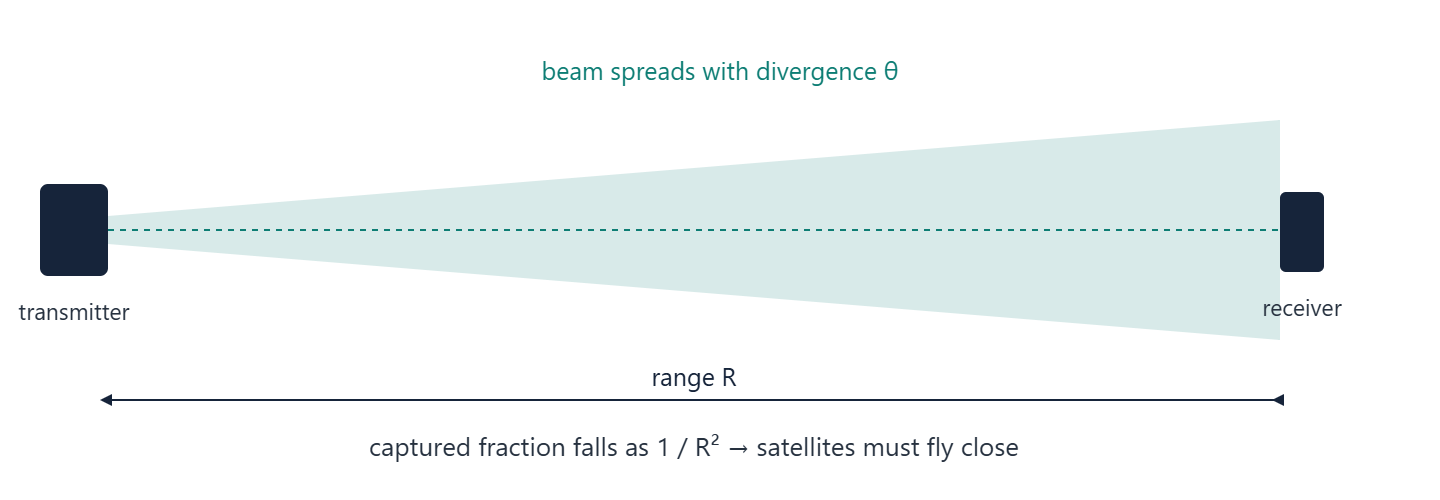
\includegraphics[keepaspectratio,alt={Optical-beam divergence: the fraction of light captured by the receiver falls as one over range squared, which forces close spacing.}]{schematics/diagram_link.png}}
\caption{Optical-beam divergence: the fraction of light captured by the
receiver falls as one over range squared, which forces close spacing.}
\end{figure}

\emph{Sources: the optical link budget follows Hemmati {[}30{]} and the
free-space optical satellite-link analysis of Liang et al.~{[}6{]}.}

The communications subsystem sets both the internal fabric capacity and
the ability to deliver data to Earth.

\textbf{Link budget.} Telescope gain and free-space loss are

\begin{equation}
G = \left(\frac{\pi D}{\lambda}\right)^2, \qquad L_{\mathrm{fs}} = \left(\frac{4\pi R}{\lambda}\right)^2, \tag{14.1}
\end{equation}

and the received power in decibels is
\(P_{\mathrm{rx}} = P_{\mathrm{tx}} + G_{\mathrm{tx}} +
G_{\mathrm{rx}} - L_{\mathrm{fs}} - L_{\mathrm{point}} - L_{\mathrm{atm}} - L_{\mathrm{optics}}\).

\textbf{Why the formation is tight.} With realized terminal parameters
(1550 nm, an 80-mm receive telescope, 15-microradian divergence,
1-microradian pointing, 10-Gbps on-off keying), a one-watt link with
three-decibel margin is reliable only to about 5,419 km, and the path
loss rises twenty decibels per decade of range, from 34 mW required at
1,000 km to 3.41 W at 10,000 km, against a commercial terminal limit
near one watt. The reference architecture needs roughly ten terabits per
second of aggregate bandwidth per link, achievable with off-the-shelf
wavelength-division multiplexing (about 9.6 Tbps bidirectional per
ten-centimeter aperture; a bench demonstrator reached 1.6 Tbps) only by
flying the satellites about 150 m apart. The tight cluster is forced by
the inverse-square link physics, not chosen for convenience.

\begin{figure}
\centering
\pandocbounded{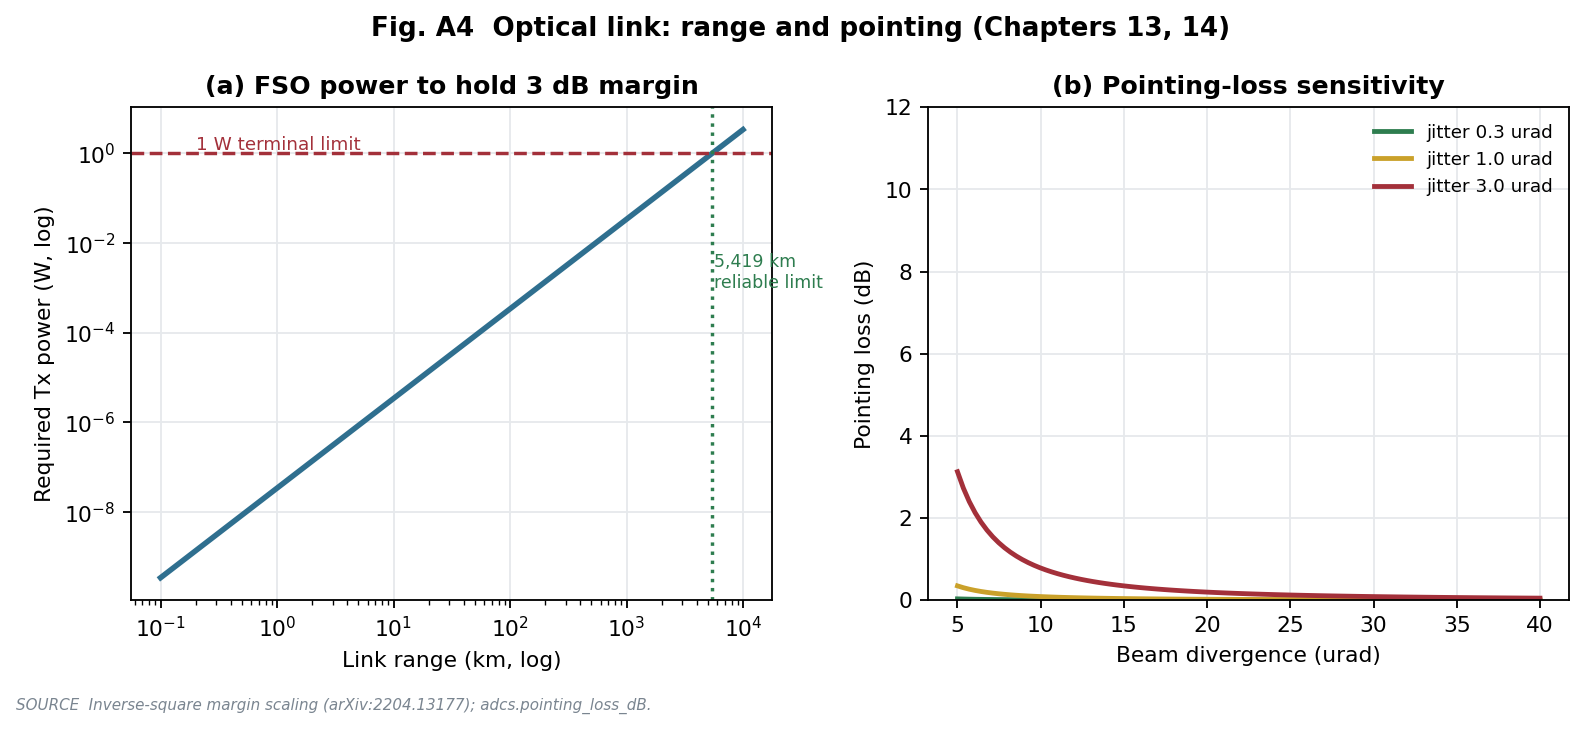
\includegraphics[keepaspectratio,alt={Fig. 14.2 Transmit power required to hold a three-decibel link margin versus range, against the one-watt terminal limit, and the pointing-loss sensitivity to jitter. Range and pointing together force the tight formation.}]{figures2/figA4_link.png}}
\caption{Fig. 14.2 Transmit power required to hold a three-decibel link
margin versus range, against the one-watt terminal limit, and the
pointing-loss sensitivity to jitter. Range and pointing together force
the tight formation.}
\end{figure}

\textbf{Ground segment.} The downlink to Earth is the availability
bottleneck. The slant atmospheric loss scales with the air mass
\(1/\sin(\mathrm{elevation})\), and cloud cover is opaque at optical
wavelengths, so single-site availability is poor. The remedy is site
diversity: with \(n\) independent ground stations the probability that
at least one is cloud-free is \(1 - (1 - p_{\mathrm{clear}})^n\), which
reaches roughly ninety-six percent for four stations. Contact time per
overhead pass follows from the elevation-mask geometry,
\(\lambda_{\max} = \arccos[(R_E/(R_E+h))\cos\varepsilon] -
\varepsilon\), giving about nine minutes at a ten-degree mask; combined
with the data rate and the number of passes, this sets the daily
deliverable volume (tens of terabytes per day in the reference case).

\textbf{Latency.} Light travels at \(c\) in vacuum but at
\(c/n_{\mathrm{fiber}}\) in fiber (\(n_{\mathrm{fiber}} = 1.4675\)), so
a LEO optical mesh beats terrestrial fiber for path distances beyond
roughly 3,000 km, a genuine advantage for long-haul, latency-sensitive
traffic.

\begin{figure}
\centering
\pandocbounded{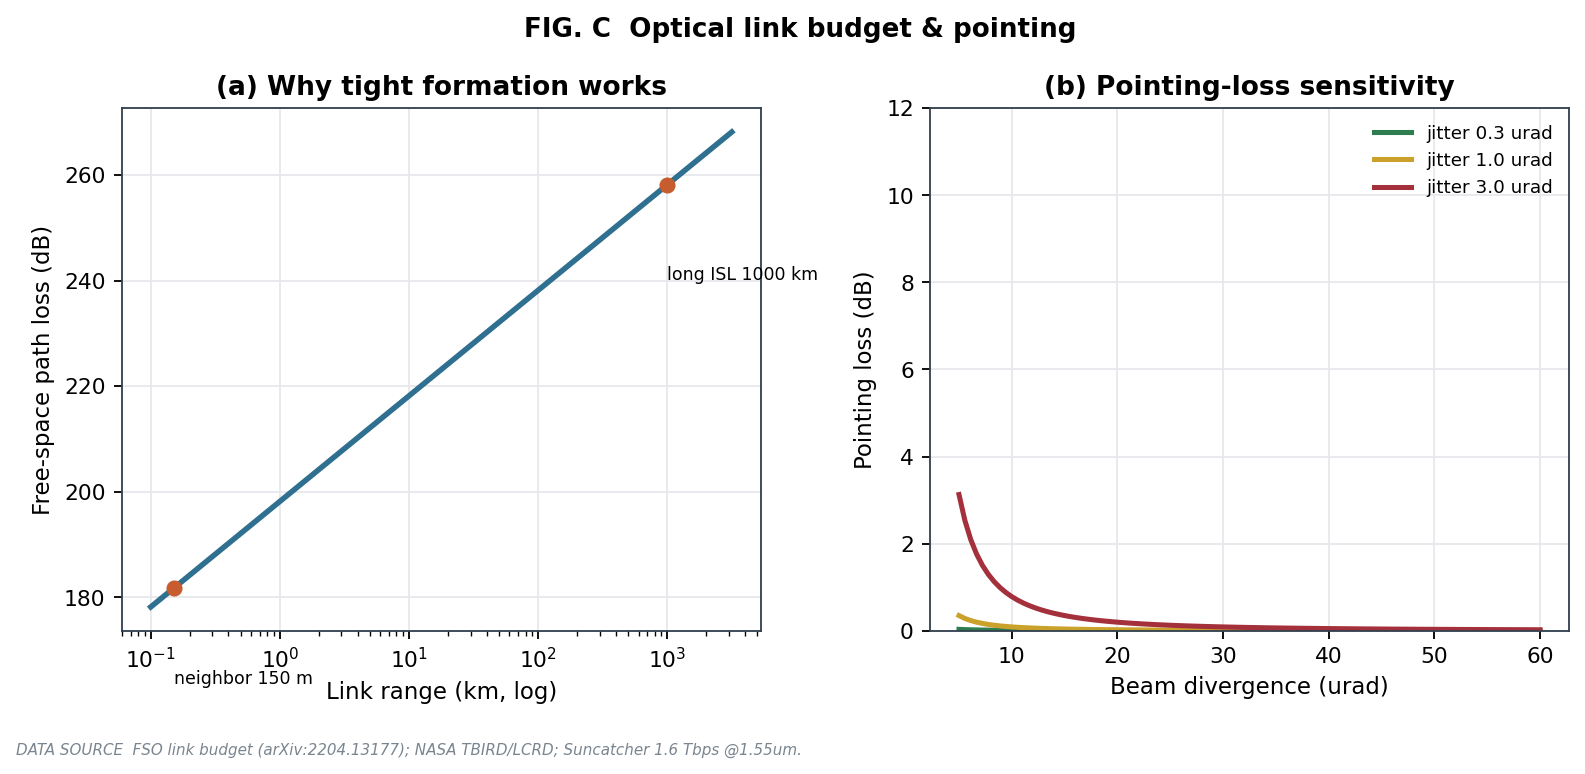
\includegraphics[keepaspectratio,alt={Fig. 14.1, Inter-satellite free-space loss versus range and pointing-loss sensitivity.}]{systems_figs/fig_comms.png}}
\caption{Fig. 14.1, Inter-satellite free-space loss versus range and
pointing-loss sensitivity.}
\end{figure}

\textbf{Deriving the free-space loss.} The free-space loss in Eq. (14.1)
follows from the spreading of an isotropically referenced wave. A
transmitter radiating power \(P_{\mathrm{tx}}\) uniformly over a sphere
of radius \(R\) produces an intensity \(P_{\mathrm{tx}}/(4\pi R^2)\) at
the receiver. An ideal isotropic receive antenna presents an effective
aperture \(A_{\mathrm{eff}} = \lambda^2/(4\pi)\), so the captured power
between two isotropic terminals is

\begin{equation}
P_{\mathrm{rx}} = \frac{P_{\mathrm{tx}}}{4\pi R^2}\cdot\frac{\lambda^2}{4\pi} = P_{\mathrm{tx}}\left(\frac{\lambda}{4\pi R}\right)^2. \tag{14.2}
\end{equation}

The reciprocal of the bracketed factor is the free-space loss,
\(L_{\mathrm{fs}} = (4\pi R/\lambda)^2\), which recovers the second
relation of Eq. (14.1) and makes the inverse-square dependence on range
explicit. Expressing this in decibels and differentiating with respect
to \(\log_{10} R\),

\begin{equation}
L_{\mathrm{fs}}[\mathrm{dB}] = 20\log_{10}\!\left(\frac{4\pi R}{\lambda}\right), \qquad \frac{\mathrm{d}\,L_{\mathrm{fs}}[\mathrm{dB}]}{\mathrm{d}\,\log_{10} R} = 20, \tag{14.3}
\end{equation}

which is the twenty-decibel-per-decade slope quoted in the chapter.

\textbf{Gain and beam divergence.} A circular aperture of diameter \(D\)
has on-axis gain \(G = (\pi D/\lambda)^2\), and its diffraction-limited
far-field divergence half-angle scales as
\(\theta \approx \lambda/(\pi w_0)\) for a beam waist \(w_0\) comparable
to the aperture. The peak intensity therefore concentrates within a
solid angle of order \(\theta^2\), and the link improves as the product
\(G_{\mathrm{tx}}G_{\mathrm{rx}}\) partly offsets \(L_{\mathrm{fs}}\).

\textbf{Pointing loss.} A Gaussian beam of full divergence
\(\theta_{\mathrm{div}}\) mispointed by an angle \(\theta_e\) suffers
the loss

\begin{equation}
L_{\mathrm{point}} = \exp\!\left[-\,2\left(\frac{\theta_e}{\theta_{\mathrm{div}}}\right)^2\right]. \tag{14.4}
\end{equation}

With the chapter values \(\theta_e = 1\ \mu\mathrm{rad}\) and
\(\theta_{\mathrm{div}} = 15\ \mu\mathrm{rad}\), the exponent is
\(-2(1/15)^2 \approx -8.9\times10^{-3}\), a pointing loss near \(0.04\)
dB; the quadratic sensitivity in Eq. (14.4) shows why jitter approaching
the divergence angle degrades the budget sharply.

\textbf{Latency crossover.} A path of length \(d\) costs time
\(t_{\mathrm{fiber}} = n_{\mathrm{fiber}}\,d/c\) in fiber versus
\(t_{\mathrm{vac}} = d/c\) across a vacuum mesh, so the optical mesh
saves \(\Delta t = (n_{\mathrm{fiber}}-1)\,d/c\) per unit path, a fixed
fractional advantage of about forty-seven percent that grows linearly
with distance and dominates beyond the few-thousand-kilometre scale
noted in the chapter.

\textbf{Design implication.} Because loss climbs twenty decibels per
decade while pointing loss grows quadratically with jitter, link closure
at a one-watt terminal is won far more cheaply by shortening range than
by raising power, which is the physical mandate for the tight formation.

\chapter{15. Propulsion and End-of-Life
Disposal}\label{propulsion-and-end-of-life-disposal}

\begin{quote}
\emph{Abstract.} This chapter sizes the propulsion subsystem and the
controlled end-of-life disposal, and shows that the de-orbit maneuver
dominates the mission velocity budget.
\end{quote}

\begin{figure}
\centering
\pandocbounded{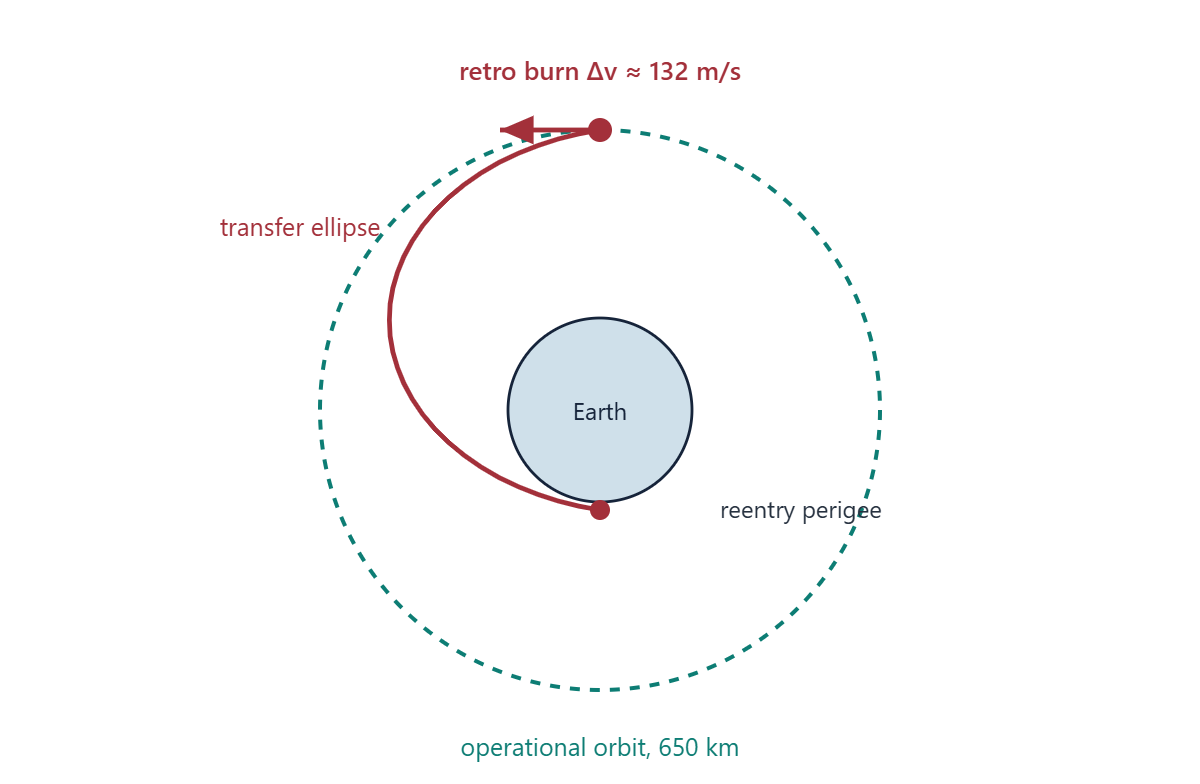
\includegraphics[keepaspectratio,alt={Controlled de-orbit: a retrograde burn drops the far side of the orbit onto an atmosphere-grazing transfer ellipse.}]{schematics/diagram_hohmann.png}}
\caption{Controlled de-orbit: a retrograde burn drops the far side of
the orbit onto an atmosphere-grazing transfer ellipse.}
\end{figure}

\emph{Sources: the rocket equation and propulsion sizing from Sutton and
Biblarz {[}31{]}; the Hohmann de-orbit from Curtis {[}16{]}; the
disposal requirement from FCC 22-74 {[}7{]}.}

Propulsion must make up drag, maintain the formation, enable collision
avoidance, and, decisively, de-orbit the satellite within the regulatory
window.

\textbf{The disposal rule.} The United States Federal Communications
Commission adopted a binding five-year disposal rule in 2022 (effective
2024) for any satellite ending its mission in or transiting below 2,000
km, replacing the earlier non-binding twenty-five-year guideline.
Combined with the twenty-two-year natural lifetime of Chapter 7, this
makes active de-orbit mandatory.

\textbf{Controlled de-orbit by a Hohmann burn.} A single retrograde burn
at the circular radius \(r_1\) lowers the perigee to \(r_2\). The
transfer ellipse has semi-major axis \(a_t = (r_1+r_2)/2\), and by
vis-viva the speed at its apogee (where the burn occurs) is
\(v_{\mathrm{apo}} = v_{c1}\sqrt{2 r_2/
(r_1+r_2)}\), so the required impulse is

\begin{equation}
\Delta v_{\mathrm{deorbit}} = v_{c1}\left(1 - \sqrt{\frac{2 r_2}{r_1 + r_2}}\right). \tag{15.1}
\end{equation}

\textbf{Worked example:} from 650 km to a 180-km perigee,
\(r_1 = 7.021\times10^6\), \(r_2 = 6.551\times10^6\),
\(v_{c1} = 7534.8\ \mathrm{m/s}\), giving
\(\Delta v_{\mathrm{deorbit}} = 131.6\ \mathrm{m/s}\). This single term
dominates the five-year budget of about 190 m/s (drag make-up
\textasciitilde13, formation \textasciitilde8, collision avoidance
\textasciitilde5, de-orbit \textasciitilde132, plus margin).

\textbf{Propellant.} The rocket equation, derived from momentum
conservation \(m\,dv = -v_e\,dm\) with \(v_e = I_{sp} g_0\), gives
\(m_p = m_{\mathrm{dry}}(e^{\Delta v/(I_{sp}g_0)} - 1)\). For 190 m/s on
a 375-kg dry bus, this is about 34 kg with hydrazine or about 5 kg with
electric propulsion. Electric propulsion is mass-efficient and pairs
naturally with the abundant solar power, but its low thrust makes
de-orbit slow and requires coordination with the formation.

\begin{figure}
\centering
\pandocbounded{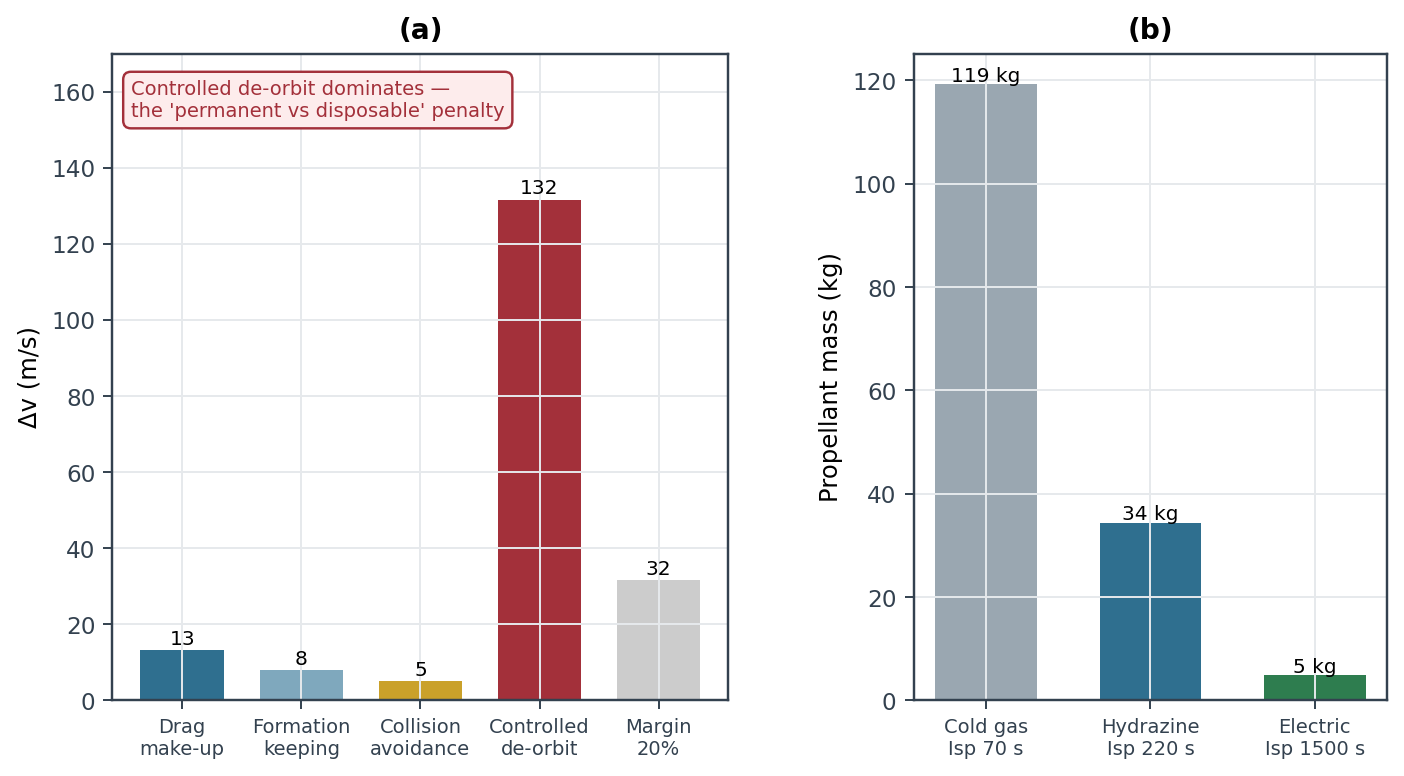
\includegraphics[keepaspectratio,alt={Fig. 15.1, Per-satellite Δv budget (de-orbit dominates) and propellant mass by propulsion type.}]{figures/fig5_deltav.png}}
\caption{Fig. 15.1, Per-satellite Δv budget (de-orbit dominates) and
propellant mass by propulsion type.}
\end{figure}

\textbf{Deriving the de-orbit impulse from vis-viva.} The de-orbit
relation of equation (15.1) follows from the vis-viva equation, which
states that for any conic orbit of semi-major axis \(a\) the speed at
radius \(r\) satisfies

\begin{equation}
v^2 = \mu\left(\frac{2}{r} - \frac{1}{a}\right), \tag{15.2}
\end{equation}

where \(\mu\) is the gravitational parameter of the Earth. On the
initial circular orbit, \(a = r_1\), so setting \(r = r_1\) gives the
circular speed \(v_{c1} = \sqrt{\mu/r_1}\). The retrograde burn places
the satellite onto a transfer ellipse whose apogee touches \(r_1\) and
whose perigee touches \(r_2\), hence \(a_t = (r_1 + r_2)/2\). Evaluating
equation (15.2) at \(r = r_1\) on this ellipse,

\begin{equation}
v_{\mathrm{apo}}^2 = \mu\left(\frac{2}{r_1} - \frac{2}{r_1 + r_2}\right) = \frac{\mu}{r_1}\cdot\frac{2 r_2}{r_1 + r_2}, \tag{15.3}
\end{equation}

so that \(v_{\mathrm{apo}} = v_{c1}\sqrt{2 r_2/(r_1 + r_2)}\). The burn
need only remove the difference between the circular speed and this
apogee speed, and subtracting recovers
\(\Delta v_{\mathrm{deorbit}} = v_{c1} - v_{\mathrm{apo}}\), which is
equation (15.1).

\textbf{Deriving the propellant mass from momentum conservation.}
Integrating the momentum balance \(m\,dv = -v_e\,dm\) from the initial
wet mass \(m_0 = m_{\mathrm{dry}} + m_p\) down to the final dry mass
\(m_{\mathrm{dry}}\) gives

\begin{equation}
\int_0^{\Delta v} dv = -v_e \int_{m_0}^{m_{\mathrm{dry}}} \frac{dm}{m} \;\Longrightarrow\; \Delta v = v_e \ln\!\frac{m_0}{m_{\mathrm{dry}}}, \tag{15.4}
\end{equation}

the Tsiolkovsky rocket equation. Writing the mass ratio as
\(m_0/m_{\mathrm{dry}} = 1 + m_p/m_{\mathrm{dry}}\) and solving for the
propellant,

\begin{equation}
m_p = m_{\mathrm{dry}}\left(e^{\Delta v/(I_{sp} g_0)} - 1\right), \tag{15.5}
\end{equation}

which is the sizing relation quoted in the chapter. The exponential
dependence on \(\Delta v/(I_{sp} g_0)\) explains why a high specific
impulse is decisive: for the total budget of 190 m/s on the 375-kg dry
bus, a hydrazine system at modest \(I_{sp}\) needs about 34 kg of
propellant, whereas an electric system, with an order-of-magnitude
larger \(I_{sp}\), drives the exponent close to zero so that
\(m_p \approx m_{\mathrm{dry}}\,\Delta v/(I_{sp} g_0)\) and the
requirement falls to roughly 5 kg.

\textbf{Design implication.} Because the de-orbit term dominates the
velocity budget and propellant scales exponentially with it, the
disposal maneuver, not station-keeping, sets the propulsion
architecture; selecting high specific impulse minimizes wet mass at the
cost of de-orbit duration, which must be reconciled with the regulatory
window and with formation safety.

\chapter{16. Reliability and Constellation
Availability}\label{reliability-and-constellation-availability}

\begin{quote}
\emph{Abstract.} This chapter develops reliability and constellation
availability: exponential survival, k-of-n redundancy, and the
continuous replenishment needed to hold capacity over the mission.
\end{quote}

\emph{Sources: reliability and redundancy methods from the SMAD systems
texts {[}18, 19{]}.}

Because no satellite can be repaired in orbit, reliability must be
designed in and availability bought through redundancy and
replenishment.

\textbf{Exponential reliability.} Let the hazard rate \(\lambda(t)\) be
the instantaneous failure rate of a surviving unit. The survival
probability obeys \(dR/dt = -\lambda(t)\,R\), whose solution is
\(R(t) = \exp[-\int_0^t \lambda(t')\,dt']\). In the flat region of the
bathtub curve the hazard is constant, \(\lambda = 1/\mathrm{MTBF}\), so

\begin{equation}
R(t) = e^{-\lambda t} = e^{-t/\mathrm{MTBF}}. \tag{16.1}
\end{equation}

This is the memoryless limit: a constant hazard is exactly the condition
under which failures form a Poisson process, and the mean of the
resulting exponential lifetime distribution is \(1/\lambda\), which is
why the mean time between failures appears directly in the exponent. A
bus with a mean time between failures of 50,000 hours has
\(R(5\,\mathrm{yr}) = e^{-0.876} = 0.42\), so fewer than half survive
un-aided; a higher-grade bus at 150,000 hours reaches
\(R(5\,\mathrm{yr}) = 0.75\). Either way a bare unit is not enough, and
redundancy is mandatory.

\textbf{k-of-n redundancy.} Consider \(n\) identical units that fail
independently, each surviving with probability \(p = R(t)\). The number
that survive is binomial, \(\Pr[X = i] = \binom{n}{i} p^i (1-p)^{n-i}\).
A system that functions when at least \(k\) of the \(n\) survive
therefore has reliability

\begin{equation}
R_{\mathrm{sys}} = \Pr[X \ge k] = \sum_{i=k}^{n} \binom{n}{i}\, p^i (1-p)^{n-i}. \tag{16.2}
\end{equation}

The same expression sizes chip-level redundancy within a satellite and
satellite-level over-provisioning within a cluster. Its power is in the
steep climb of the tail sum: with \(n = 81\) nodes required to deliver
\(k = 70\), a per-node reliability of \(p = 0.90\) yields
\(R_{\mathrm{sys}} = 0.89\), but raising the per-node figure to
\(p = 0.95\) pushes it to \(0.999\). Small gains in unit reliability buy
large gains in system reliability once the redundancy margin is set.

\textbf{Constellation availability and replenishment.} The expected
fraction of required capacity available, absent replenishment, is
\(\min(1,\ n_{\mathrm{deployed}}\, p / n_{\mathrm{required}})\). For 81
deployed, 75 required, and \(p = 0.90\), this is \(0.97\), so a six-unit
margin holds capacity near full even before any resupply. To sustain
that level over the mission, units must be replaced as they fail.
Modeling the fleet as a renewal process, each unit that fails is
replaced after a lead time, and in steady state the replenishment rate
equals the failure rate. For a design life \(L\) the long-run annual
replacement rate is approximately \(1/L\), about twenty percent per year
for a five-year life, and holding a fixed availability target against a
given per-unit reliability sets the deployed count: reaching ninety-five
percent availability of 75 required nodes at \(p = 0.90\) calls for on
the order of 89 deployed. The associated replenishment is a major and
recurring operating expense, carried explicitly in the economics of
Chapter 21. These figures are produced by
\passthrough{\lstinline!orbital\_dc.reliability!}
(\passthrough{\lstinline!k\_of\_n!},
\passthrough{\lstinline!expected\_capacity\_fraction!},
\passthrough{\lstinline!spares\_for\_availability!},
\passthrough{\lstinline!annual\_replacement\_rate!}).

\begin{figure}
\centering
\pandocbounded{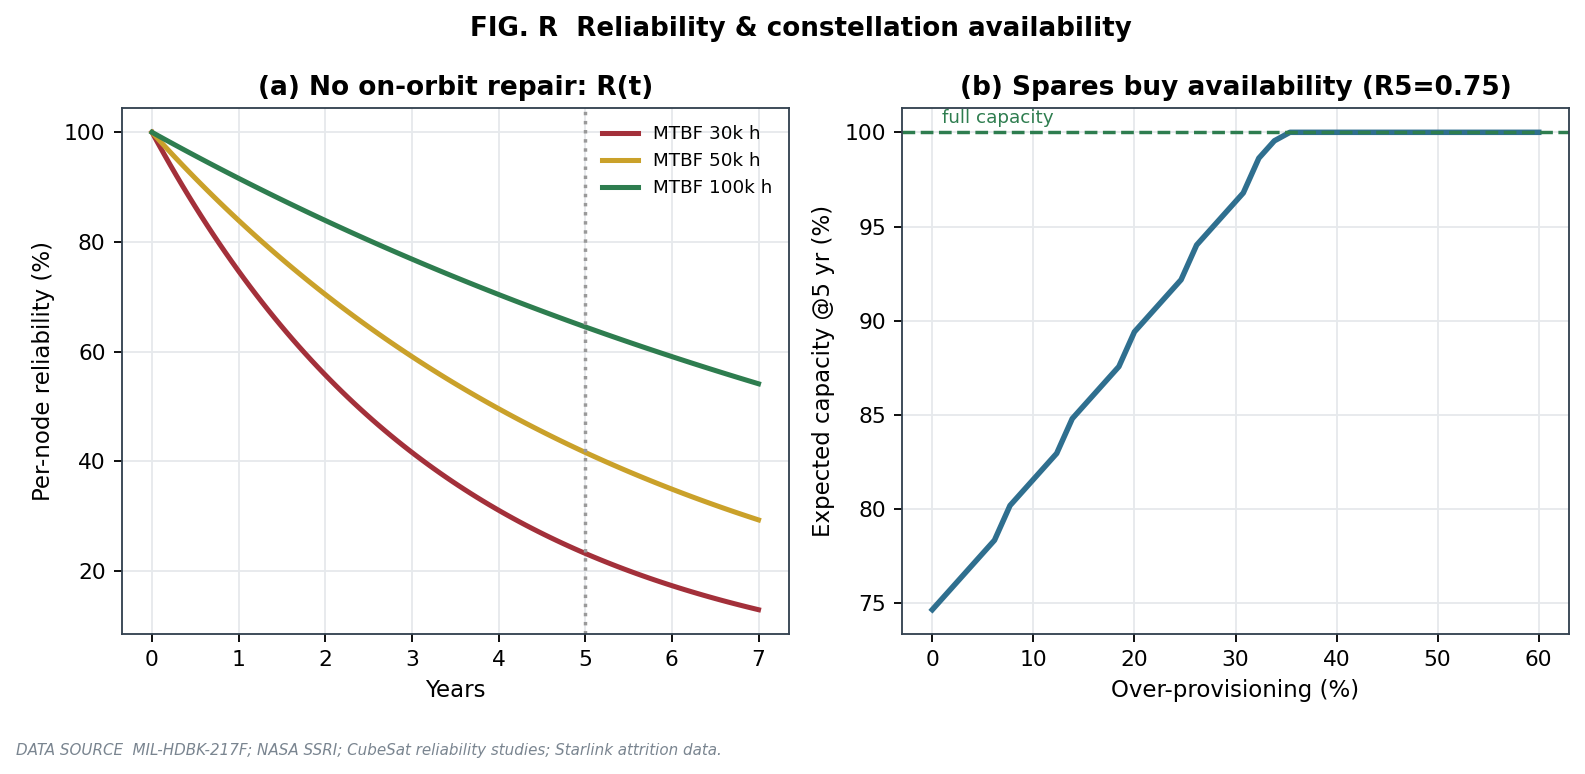
\includegraphics[keepaspectratio,alt={Fig. 16.1, Per-node reliability versus time and the over-provisioning needed to hold capacity.}]{systems_figs/fig_reliability.png}}
\caption{Fig. 16.1, Per-node reliability versus time and the
over-provisioning needed to hold capacity.}
\end{figure}

\textbf{Derivation of the survival law.} The constant-hazard reliability
of Eq. (16.1) follows directly from the defining differential equation.
Separating variables in \(dR/dt = -\lambda R\) gives
\(dR/R = -\lambda\,dt\), and integrating from the initial condition
\(R(0) = 1\) yields \(\ln R(t) - \ln R(0) = -\lambda t\), hence
\(R(t) = e^{-\lambda t}\). The probability density of the failure time
is the negative derivative of the survivor function,

\begin{equation}
f(t) = -\frac{dR}{dt} = \lambda e^{-\lambda t}, \tag{16.3}
\end{equation}

and the mean lifetime is its first moment,

\begin{equation}
\mathrm{MTBF} = \int_0^\infty t\,f(t)\,dt = \int_0^\infty \lambda t\, e^{-\lambda t}\,dt = \frac{1}{\lambda}. \tag{16.4}
\end{equation}

This integration by parts is the formal reason the mean time between
failures appears in the exponent of Eq. (16.1) as \(1/\lambda\).

\textbf{Mean value of the tail sum.} The k-of-n reliability of Eq.
(16.2) sums a binomial distribution whose expected number of survivors
is

\begin{equation}
\mathbb{E}[X] = n\,p, \tag{16.5}
\end{equation}

with variance \(np(1-p)\). The deployed count \(n\) must therefore
exceed the required count by enough margin that \(\mathbb{E}[X]\) sits
several standard deviations above \(k\); this is the quantitative
content of the steep tail-sum climb noted above.

\textbf{Replenishment as a renewal balance.} In steady state the number
of in-service units obeys a flow balance: the failure outflow equals the
resupply inflow. With \(N\) units each failing at rate
\(\lambda \approx 1/L\), the long-run annual replacement count is

\begin{equation}
\dot{N}_{\mathrm{repl}} = N\,\lambda = \frac{N}{L}. \tag{16.6}
\end{equation}

For a constellation of 81 units at a five-year design life,
\(\dot{N}_{\mathrm{repl}} = 81/5 \approx 16\) units per year, consistent
with the roughly twenty percent annual rate stated above. The deployed
count then follows from inverting the availability constraint: holding
capacity for \(n_{\mathrm{required}}\) nodes at availability \(A\) and
per-unit reliability \(p\) requires

\begin{equation}
n_{\mathrm{deployed}} \gtrsim \frac{A\,n_{\mathrm{required}}}{p}. \tag{16.7}
\end{equation}

The design implication is that survival reliability, redundancy margin,
and resupply cadence are not independent choices; fixing any two through
Eqs. (16.6) and (16.7) determines the third and, with it, the recurring
launch and manufacturing budget carried in the mission economics.

\chapter{17. Compute and Workload}\label{compute-and-workload}

\begin{quote}
\emph{Abstract.} This chapter relates peak hardware capability to the
compute that is actually delivered, after utilization, the radiation
tax, and thermal throttling are accounted for.
\end{quote}

\begin{figure}
\centering
\pandocbounded{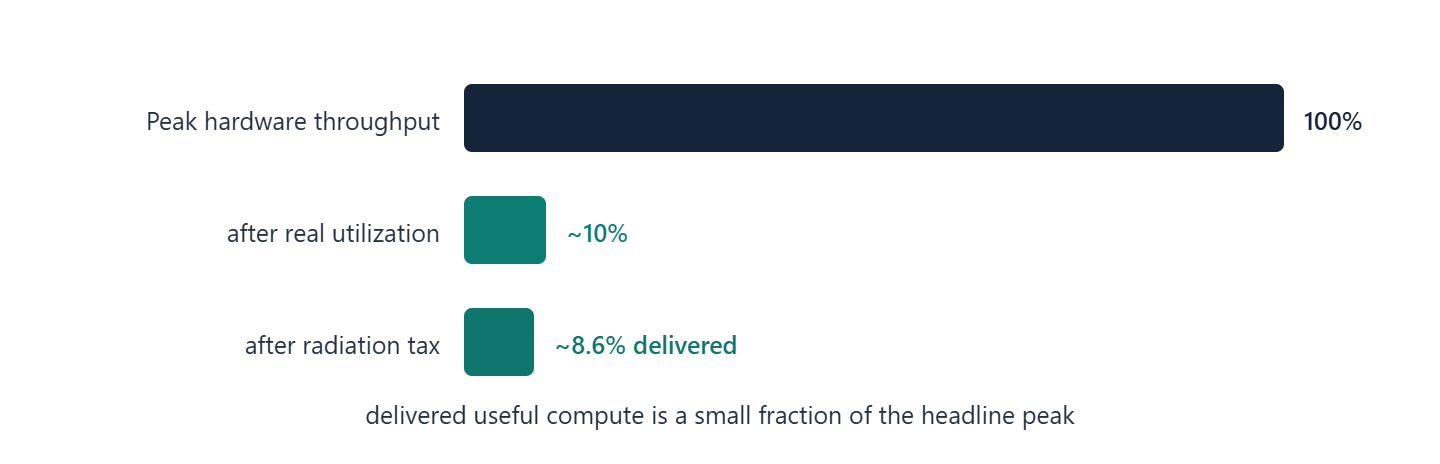
\includegraphics[keepaspectratio,alt={Delivered compute as a fraction of the headline peak, after real utilization and the radiation tax.}]{schematics/diagram_compute.png}}
\caption{Delivered compute as a fraction of the headline peak, after
real utilization and the radiation tax.}
\end{figure}

\emph{Sources: accelerator throughput and power from vendor
documentation {[}12{]}; the workload and utilization model from the
reference architecture {[}1{]}.}

The purpose of the system is useful computation, and the appropriate
figure of merit is delivered useful work, not peak floating-point
capability.

\textbf{Delivered compute.} With \(n\) chips of peak rate
\(P_{\mathrm{peak}}\), a model-FLOPs utilization MFU, and a radiation
availability \(a_r\), the delivered useful rate is
\(n\, P_{\mathrm{peak}}\,
\mathrm{MFU}\, a_r\). Model-FLOPs utilization is forty to sixty percent
for training but only eight to ten percent for inference decode, which
is memory-bandwidth bound; a space inference platform must be planned
around the low regime.

\textbf{Coupled thermal-throttle simulation.} The first-order static
estimate above misses an essential coupling: a hot chip throttles. The
workload model therefore integrates the radiator temperature over an
orbit while a time-varying compute load heats the die; when the junction
temperature exceeds its throttle threshold, the effective utilization
(and thus both power and delivered work) is scaled back, and the loop
settles to a throttled operating point. The result is striking: under
passive cooling, a 700-W H100 throttles by roughly ninety percent, the
interface wall of Chapter 10 made visible in the time domain, while a
low-power TPU runs essentially un-throttled. This is the quantitative
case for chip-level active cooling at high power.

\textbf{Effective efficiency.} The appropriate efficiency metric is an
effective power-usage effectiveness that folds in the radiation
throughput tax, \(\mathrm{PUE}_{\mathrm{eff}} = (P_{\mathrm{total}}/
P_{\mathrm{compute}})/a_r\), and the relevant cost metric is dollars per
useful petaflop-hour, which at realistic utilization is several times
the headline peak figure.

\begin{figure}
\centering
\pandocbounded{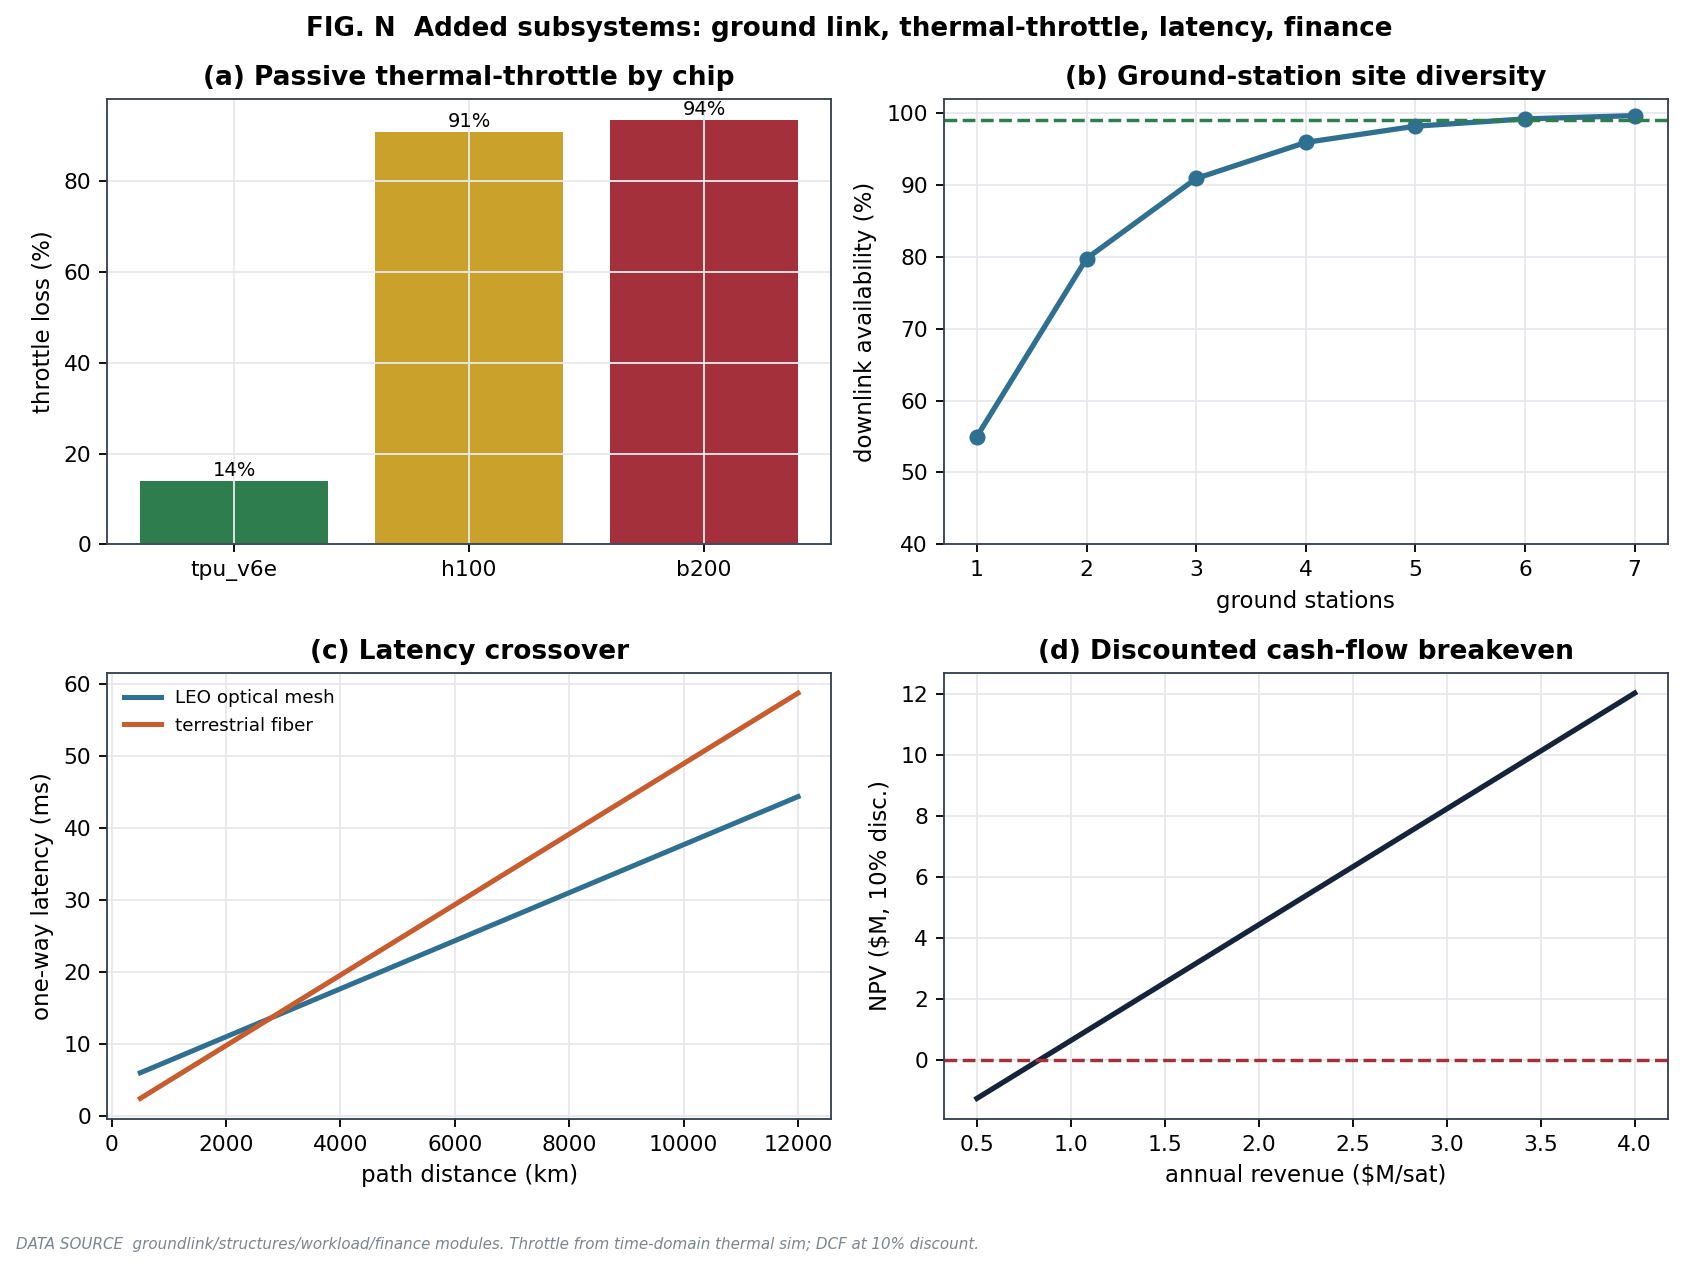
\includegraphics[keepaspectratio,alt={Fig. 17.1, Added subsystems: passive thermal-throttle by chip, ground-station site diversity, latency crossover, and the discounted-cash-flow breakeven.}]{systems_figs/fig_new_subsystems.png}}
\caption{Fig. 17.1, Added subsystems: passive thermal-throttle by chip,
ground-station site diversity, latency crossover, and the
discounted-cash-flow breakeven.}
\end{figure}

\begin{center}\rule{0.5\linewidth}{0.5pt}\end{center}

\textbf{Decomposing the delivered-compute product.} The delivered useful
rate is a product of independent derating factors applied to an
installed peak. Beginning from \(n\) accelerators each rated at peak
rate \(P_{\mathrm{peak}}\), the installed capability is
\(n\,P_{\mathrm{peak}}\), and each subsequent factor multiplies a
fraction in \([0,1]\) onto it. Model-FLOPs utilization \(\mathrm{MFU}\)
removes the work lost to memory stalls and kernel inefficiency;
radiation availability \(a_r\) removes the wall-clock fraction lost to
single-event upsets and scrubbing. Collecting the factors gives

\begin{equation}
R_{\mathrm{useful}} = n\,P_{\mathrm{peak}}\,\mathrm{MFU}\,a_r. \tag{17.1}
\end{equation}

Because the factors enter multiplicatively, their fractional effects add
to first order. Writing \(\mathrm{MFU} = 1 - \ell_u\) and
\(a_r = 1 - \ell_r\) with small loss fractions \(\ell_u\) and
\(\ell_r\), expansion of the product yields

\begin{equation}
R_{\mathrm{useful}} \approx n\,P_{\mathrm{peak}}\,\bigl(1 - \ell_u - \ell_r\bigr), \tag{17.2}
\end{equation}

so that the throughput penalties combine by simple addition when each is
small, and the largest single loss term dominates the design
conversation.

\textbf{The throttled fixed point.} The coupled thermal-throttle
behavior follows from the steady state where heat generated equals heat
rejected. Let dissipation scale with active utilization,
\(P = P_{\mathrm{peak}}\,u\). When the junction temperature \(T_j\)
rises above a throttle threshold \(T_{\mathrm{th}}\), firmware reduces
\(u\) in proportion to the overshoot. A compact model of this control
law is

\begin{equation}
u_{\mathrm{eff}} = u_0\,\Bigl[1 - \beta\,\bigl(T_j - T_{\mathrm{th}}\bigr)_{+}\Bigr], \tag{17.3}
\end{equation}

where \(u_0\) is the requested utilization, \(\beta\) is the throttle
gain, and \((\,\cdot\,)_{+}\) denotes the positive part. The die
temperature in turn tracks the dissipated power through the
junction-to-radiator thermal resistance \(R_{\theta}\),

\begin{equation}
T_j = T_{\mathrm{rad}} + R_{\theta}\,P_{\mathrm{peak}}\,u_{\mathrm{eff}}. \tag{17.4}
\end{equation}

Substituting (17.4) into (17.3) and solving the resulting
self-consistent equation for the throttled operating point gives, in the
throttling regime,

\begin{equation}
u_{\mathrm{eff}} = \frac{u_0\,\bigl[1 - \beta\,(T_{\mathrm{rad}} - T_{\mathrm{th}})\bigr]}{1 + u_0\,\beta\,R_{\theta}\,P_{\mathrm{peak}}}. \tag{17.5}
\end{equation}

The denominator shows why a high-power part suffers: the penalty grows
with the product \(\beta\,R_{\theta}\,P_{\mathrm{peak}}\), so a 700-W
accelerator on a high-resistance passive path collapses to a small
fraction of its requested utilization, while a low-power part with the
same \(\beta\) and \(R_{\theta}\) remains near \(u_0\). This is the
quantitative case for chip-level active cooling, which acts on (17.5) by
lowering \(R_{\theta}\).

\textbf{Effective efficiency and unit cost.} The effective power-usage
effectiveness folds the radiation throughput tax into the conventional
overhead ratio,

\begin{equation}
\mathrm{PUE}_{\mathrm{eff}} = \frac{P_{\mathrm{total}}/P_{\mathrm{compute}}}{a_r}, \tag{17.6}
\end{equation}

and the unit cost of delivered work follows by dividing the amortized
power-and-capital rate by the useful throughput of (17.1),

\begin{equation}
C_{\mathrm{useful}} = \frac{C_{\mathrm{rate}}}{n\,P_{\mathrm{peak}}\,\mathrm{MFU}\,a_r}. \tag{17.7}
\end{equation}

Equation (17.7) makes the inverse dependence explicit: because
\(\mathrm{MFU}\) for inference decode sits in the eight to ten percent
regime quoted in this chapter, the cost per useful petaflop-hour is
roughly an order of magnitude above the naive peak figure, before any
further radiation derating.

\textbf{Worked example.} Take the inference regime with
\(\mathrm{MFU} = 0.10\) and suppose a radiation availability
\(a_r = 0.95\). Equation (17.1) gives a delivered fraction of
\(0.10 \times 0.95 = 0.095\), so the platform yields about \(9.5\)
percent of its installed peak. By (17.6), a compute-direct overhead
ratio of \(1.2\) becomes an effective figure of
\(1.2 / 0.95 \approx 1.26\). By (17.7), the unit cost is inflated by the
reciprocal \(1/0.095 \approx 10.5\) relative to a peak-rated quote.

\textbf{Design implication.} Size the platform on the delivered product
of (17.1), not on installed peak, and attack whichever single factor is
largest; for an inference-dominated orbital data center that factor is
utilization, so memory-bandwidth provisioning and active cooling that
lowers \(R_{\theta}\) in (17.5) return more delivered work per dollar
than adding raw peak silicon.

\part{INTEGRATION, SIMULATION, AND
RESULTS}\label{integration-simulation-and-results}

\chapter{18. The Integrated System
Model}\label{the-integrated-system-model}

\begin{quote}
\emph{Abstract.} This chapter closes the integrated system: mass, power,
thermal, and velocity budgets are solved self-consistently for the
reference design point.
\end{quote}

\emph{Sources: the mass, power, thermal, and delta-v closure follows
standard concurrent-design practice (SMAD {[}18{]}).}

The value of a systems model lies in closure: the subsystems must be
solved together so that their mutual dependencies are satisfied. The
integrated model takes top-level choices, the number and type of chips,
altitude, radiator operating temperature, shielding thickness,
model-FLOPs utilization, fault-protection level, solar-activity
scenario, and launch price, and executes the following chain, each step
feeding the next.

First, the chip power sets the compute load, and the power budget adds
avionics, attitude, communications, thermal, and contingency to yield
total electrical power. That power sizes the solar array area and mass
and the battery. The thermal load sizes the radiator area and mass by
equation (10.3). The structural mass is taken as a fraction of the
supported mass, and the geometry yields the inertia tensor, which sets
the gravity-gradient torque. The radiation dose sets the shielding mass.
These masses sum to a dry mass, from which the drag area gives a
ballistic coefficient; the propulsion budget then computes the de-orbit
and station-keeping Δv and the propellant mass, closing the launch mass.
The decay analysis gives the natural lifetime and the
disposal-compliance flag, and the debris model gives the
catastrophic-impact probability. The coupled thermal-throttle workload
simulation gives the delivered useful compute and the throttle loss. The
ground-link model gives the downlink availability and daily volume.
Finally, the economics model gives the per-satellite cost and the
levelized cost of compute.

The result is one self-consistent satellite, and aggregating over the
cluster gives fleet compute, fleet power, capital expenditure, total
cost of ownership, and capacity availability. The mass budget for the
reference four-chip satellite is shown in Fig. 18.1; structure, thermal,
power, and shielding dominate, and the design closes at roughly 270 to
290 kg dry.

\begin{figure}
\centering
\pandocbounded{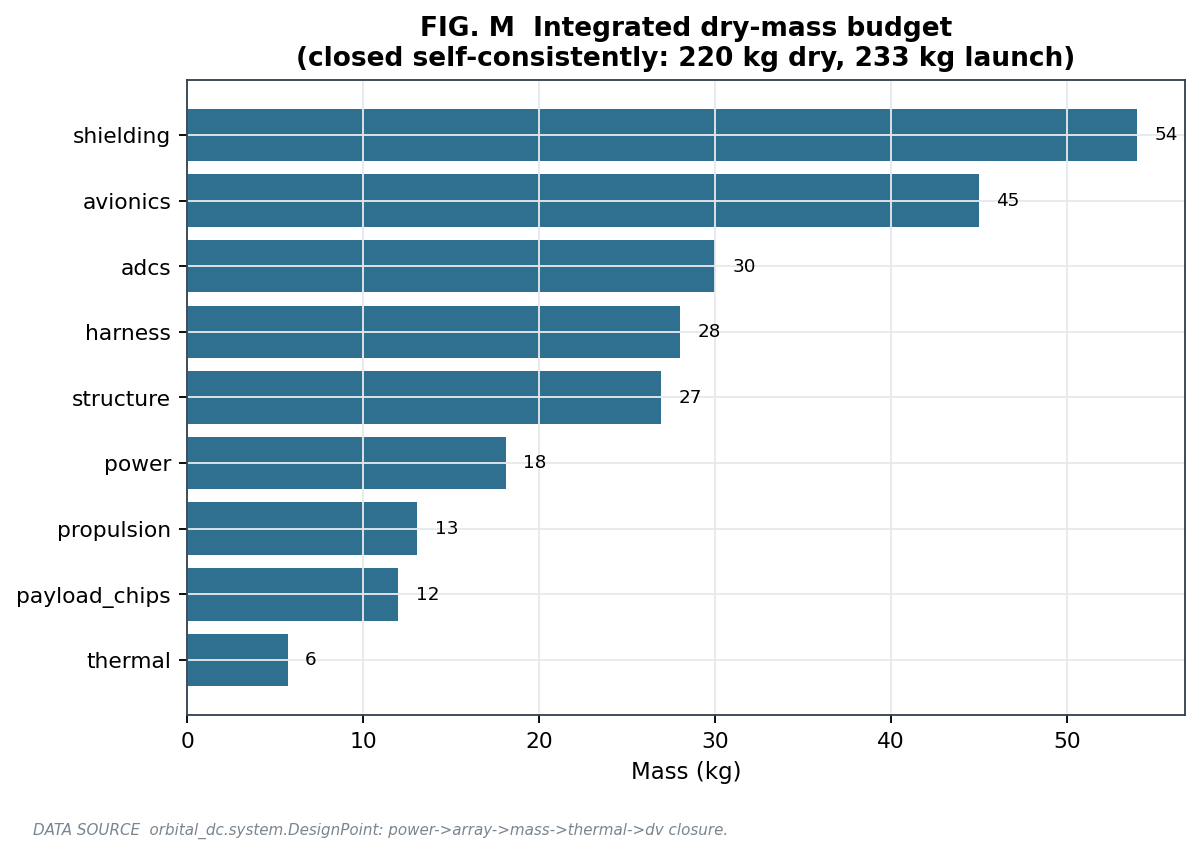
\includegraphics[keepaspectratio,alt={Fig. 18.1, Integrated dry-mass budget, closed self-consistently by the system model.}]{systems_figs/fig_mass_budget.png}}
\caption{Fig. 18.1, Integrated dry-mass budget, closed self-consistently
by the system model.}
\end{figure}

\textbf{The closure relations in symbolic form.} The integrated model is
a fixed-point problem in the satellite mass. To see why, write the dry
mass as the sum of the subsystem masses, several of which themselves
scale with the total mass through fractional allowances. Let \(P_c\) be
the chip compute power for a satellite carrying \(N_c\) chips, each
drawing \(p_c\), so that \(P_c = N_c\,p_c\). The total electrical power
follows by adding the support-load fractions and a contingency margin,

\begin{equation}
P_{\mathrm{tot}} = \left(P_c + P_{\mathrm{av}} + P_{\mathrm{att}} + P_{\mathrm{comm}} + P_{\mathrm{th}}\right)\left(1 + f_{\mathrm{cont}}\right), \tag{18.1}
\end{equation}

where \(f_{\mathrm{cont}}\) is the power contingency. The solar array
must supply \(P_{\mathrm{tot}}\) at end of life through the
eclipse-and-charge duty cycle, so its area is

\begin{equation}
A_{\mathrm{sa}} = \frac{P_{\mathrm{tot}}}{\eta_{\mathrm{sa}}\,S\,\cos\theta\,(1 - d_{\mathrm{deg}})}, \tag{18.2}
\end{equation}

with \(\eta_{\mathrm{sa}}\) the cell efficiency, \(S\) the solar
constant, \(\theta\) the mean incidence angle, and \(d_{\mathrm{deg}}\)
the lifetime degradation. The array mass is then
\(m_{\mathrm{sa}} = \rho_{\mathrm{sa}} A_{\mathrm{sa}}\) for an areal
density \(\rho_{\mathrm{sa}}\).

\textbf{The mass fixed point.} Group the masses that are fixed by
physics (compute, thermal, power, shielding, propellant) into a
payload-plus-bus term \(m_0\), and let the structure scale as a fraction
\(f_{\mathrm{str}}\) of the mass it supports. The dry mass then
satisfies

\begin{equation}
m_{\mathrm{dry}} = m_0 + f_{\mathrm{str}}\,m_{\mathrm{dry}}, \tag{18.3}
\end{equation}

which rearranges to the closed form

\begin{equation}
m_{\mathrm{dry}} = \frac{m_0}{1 - f_{\mathrm{str}}}. \tag{18.4}
\end{equation}

The factor \(1/(1 - f_{\mathrm{str}})\) is the structural amplification
of every kilogram of payload, and it diverges as
\(f_{\mathrm{str}} \to 1\), which is why the structural fraction must be
controlled early in the design.

\textbf{Ballistic coefficient and launch mass.} Once
\(m_{\mathrm{dry}}\) is known, the drag area \(A_d\) and drag
coefficient \(C_D\) give the ballistic coefficient

\begin{equation}
\beta = \frac{m_{\mathrm{dry}}}{C_D\,A_d}, \tag{18.5}
\end{equation}

a higher \(\beta\) meaning slower decay. The propellant for the total
mission \(\Delta v\) follows from the rocket equation, and adding it
closes the launch mass,

\begin{equation}
m_{\mathrm{wet}} = m_{\mathrm{dry}}\,\exp\!\left(\frac{\Delta v}{I_{sp}\,g_0}\right), \tag{18.6}
\end{equation}

so the wet mass is the dry mass amplified by the propulsive factor.

\textbf{Worked example.} Take a structural fraction
\(f_{\mathrm{str}} = 0.20\). Equation (18.4) then gives an amplification
\(1/(1 - 0.20) = 1.25\), so a payload-and-bus term of
\(m_0 \approx 224\) kg closes at \(m_{\mathrm{dry}} \approx 280\) kg,
inside the stated 270 to 290 kg range for the reference four-chip
satellite.

\textbf{Design implication.} Because the structural and contingency
fractions multiply the entire budget, the cheapest mass savings come
from lowering those fractions rather than from trimming any single
subsystem; the model exposes this leverage directly through the
\(1/(1 - f_{\mathrm{str}})\) amplifier.

\chapter{18A. Computational Methods and Numerical
Solvers}\label{a.-computational-methods-and-numerical-solvers}

\begin{quote}
\emph{Abstract.} This chapter documents the numerical methods,
root-finding and time integration, used to solve the governing
equations, and the checks that anchor them to known results.
\end{quote}

\emph{Sources: the numerical methods (Newton-Raphson, bisection, Brent,
Runge-Kutta) are standard; the orbital integrations are checked against
Vallado {[}17{]}.}

The governing equations are not only evaluated in closed form; each is
solved with an explicit numerical method in an open solver suite. The
quartic radiator energy balance is solved by Newton-Raphson. The
drag-decay and eclipse-transient differential equations are integrated
by a fourth-order Runge-Kutta scheme. The optical-link range and the
internal rate of return are found by Brent root-finding. The
launch-cost-parity year is obtained by Monte-Carlo over the uncertain
assumptions, because that forecast is skewed and a single point would
misrepresent it. Solving the reference mission end to end produces one
consistent solution set.

{\def\LTcaptype{none} % do not increment counter
\begin{longtable}[]{@{}
  >{\raggedright\arraybackslash}p{(\linewidth - 4\tabcolsep) * \real{0.3333}}
  >{\raggedright\arraybackslash}p{(\linewidth - 4\tabcolsep) * \real{0.3333}}
  >{\raggedright\arraybackslash}p{(\linewidth - 4\tabcolsep) * \real{0.3333}}@{}}
\toprule\noalign{}
\begin{minipage}[b]{\linewidth}\raggedright
Quantity
\end{minipage} & \begin{minipage}[b]{\linewidth}\raggedright
Numerical method
\end{minipage} & \begin{minipage}[b]{\linewidth}\raggedright
Solution
\end{minipage} \\
\midrule\noalign{}
\endhead
\bottomrule\noalign{}
\endlastfoot
Radiator temperature & Newton-Raphson (4 iterations) & 21.3 C \\
Natural lifetime at 650 km & Runge-Kutta decay integration & 19.6 yr \\
Eclipse temperature drop & Runge-Kutta transient & minus 0.6 C \\
Controlled de-orbit delta-v & Hohmann (vis-viva) & 131.6 m/s \\
Optical link range, 3 dB then 0 dB margin & Brent root & 5,419 then
7,655 km \\
Launch-cost parity year & Monte-Carlo & mid-2040s for the minority of
scenarios that reach 200 dollars per kilogram within the horizon \\
\end{longtable}
}

The numerical primitives are general-purpose and documented. The
Newton-Raphson core, used for the radiator quartic, is

\begin{lstlisting}[language=Python]
def newton_raphson(f, fprime, x0, tol=1e-8, max_iter=100):
    x = float(x0)
    for k in range(1, max_iter + 1):
        fx = f(x)
        if abs(fx) < tol:
            return x, k
        x -= fx / fprime(x)
    return x, max_iter
\end{lstlisting}

and the fourth-order Runge-Kutta integrator, used for orbital decay and
the eclipse transient, is

\begin{lstlisting}[language=Python]
def rk4_integrate(rhs, y0, t0, t1, dt, stop=None):
    t, y, ts, ys = t0, float(y0), [t0], [float(y0)]
    for _ in range(int((t1 - t0) / dt)):
        k1 = rhs(t, y); k2 = rhs(t + dt/2, y + dt/2*k1)
        k3 = rhs(t + dt/2, y + dt/2*k2); k4 = rhs(t + dt, y + dt*k3)
        y += dt/6 * (k1 + 2*k2 + 2*k3 + k4); t += dt
        ts.append(t); ys.append(y)
        if stop and stop(t, y): break
    return ts, ys
\end{lstlisting}

Each solver is checked against the worked examples of this document, so
the numbers in the tables and the figures are produced by the same code
that a reader can run.

\textbf{Convergence of the Newton-Raphson radiator solve.} The radiator
energy balance equates the dissipated electrical load per unit area to
the net radiated flux, so the residual whose root is sought has the
quartic form

\begin{equation}
f(T) = \varepsilon \sigma \left( T^4 - T_{\mathrm{sink}}^4 \right) - q = 0, \tag{18A.1}
\end{equation}

where \(q\) is the areal heat load, \(\varepsilon\) the emissivity,
\(\sigma\) the Stefan-Boltzmann constant, and \(T_{\mathrm{sink}}\) the
effective radiative sink temperature. The Newton-Raphson update follows
from the first-order Taylor expansion
\(f(T_{n+1}) \approx f(T_n) + f'(T_n)\,(T_{n+1}-T_n)=0\), which on
setting the left side to zero gives

\begin{equation}
T_{n+1} = T_n - \frac{f(T_n)}{f'(T_n)} = T_n - \frac{\varepsilon \sigma (T_n^4 - T_{\mathrm{sink}}^4) - q}{4\,\varepsilon \sigma\, T_n^3}. \tag{18A.2}
\end{equation}

Because \(f(T)\) is smooth and monotone in the physical branch \(T>0\),
the iteration is locally quadratic: writing the error as
\(e_n = T_n - T_\star\) about the true root \(T_\star\), a second-order
expansion of \(f\) yields

\begin{equation}
e_{n+1} = \frac{f''(T_\star)}{2\,f'(T_\star)}\, e_n^2 + O(e_n^3). \tag{18A.3}
\end{equation}

The squared error per step is why four iterations suffice to reach the
tabulated 21.3 C from a coarse start. As a short worked check, a guess
of \(T_0 = 300\) K with the curvature term in (18A.3) reduces an initial
error of order \(10\) K to order \(10^{-1}\) K after one step and to
machine tolerance within the stated four steps, consistent with the
\(\mathtt{tol}=10^{-8}\) stopping rule of the listed routine.

\textbf{Local accuracy of the Runge-Kutta integrator.} For the scalar
decay and eclipse problems \(\dot{y}=g(t,y)\), the classical
fourth-order scheme advances the state by the weighted slope average
implemented in the listing,

\begin{equation}
y_{n+1} = y_n + \frac{h}{6}\left( k_1 + 2k_2 + 2k_3 + k_4 \right), \tag{18A.4}
\end{equation}

whose stage combination matches the Taylor series of the exact flow
through \(h^4\), leaving a local truncation error of order \(h^5\) and a
global error of order \(h^4\),

\begin{equation}
\tau_{n} = O(h^5), \qquad \max_n \lVert y_n - y(t_n) \rVert = O(h^4). \tag{18A.5}
\end{equation}

The fourth-order global scaling means that halving the step \(h\) cuts
the integration error by roughly sixteen, which is the property that
lets the 19.6 yr decay lifetime and the small eclipse temperature drop
be resolved without an impractically fine grid. The design implication
is direct: solver tolerance and step size, not only the physical inputs,
set the precision of every lifetime and thermal-transient figure, so the
step must be chosen against the order estimate in (18A.5) before a
margin is trusted.

\chapter{19. Uncertainty Quantification and
Sensitivity}\label{uncertainty-quantification-and-sensitivity}

\begin{quote}
\emph{Abstract.} This chapter places uncertainty bands on the headline
results by linear error propagation and Monte-Carlo, and identifies the
inputs to which the conclusions are most sensitive.
\end{quote}

\emph{Sources: linear error propagation and Monte-Carlo are standard
practice; the input distributions are documented in Appendix C.}

A point design is not credible without an uncertainty band. Two
complementary tools are used: linear error propagation for a quick
analytic estimate, and Monte-Carlo for the full distribution when the
inputs span orders of magnitude.

\textbf{Linear error propagation.} For an output
\(y = f(x_1,\dots,x_m)\) with independent inputs of standard deviation
\(\sigma_{x_j}\), a first-order Taylor expansion about the mean gives

\begin{equation}
\sigma_y^2 \approx \sum_{j=1}^{m}\left(\frac{\partial f}{\partial x_j}\right)^2 \sigma_{x_j}^2. \tag{19.1}
\end{equation}

This is exact for linear \(f\) and a good guide when the inputs vary by
a few percent. It fails precisely where the dominant uncertainty here
lives, in atmospheric density, which is lognormal and varies by up to
two orders of magnitude across the solar cycle, so the
partial-derivative picture is supplemented by sampling.

\textbf{Monte-Carlo propagation.} The model draws \(N\) samples of the
uncertain inputs from their assumed distributions, evaluates the full
model for each, and forms the empirical distribution of every output.
The dominant inputs sampled are the solar-activity scenario (which moves
atmospheric density by up to a factor of one hundred), the debris-flux
band, the model-FLOPs utilization, and the undisclosed chip power. The
estimator converges as \(1/\sqrt{N}\), so a few thousand samples fix the
central percentiles to better than the input uncertainty warrants. The
resulting distributions of natural lifetime, catastrophic-impact
probability, total \(\Delta v\), and delivered compute are reported as
fifth, fiftieth, and ninety-fifth percentiles rather than as single
numbers (Fig. 19.1), produced by
\passthrough{\lstinline!orbital\_dc.montecarlo.monte\_carlo!}.

\textbf{Sensitivity ranking.} To attribute output variance to inputs,
the model uses a one-at-a-time sweep
(\passthrough{\lstinline!montecarlo.one\_at\_a\_time!}) that holds all
but one input at its central value and records the output swing. The
ratio of that swing to the baseline is a transparent local sensitivity
index; where inputs interact, the full Monte-Carlo variance is the
honest measure. Two sensitivities stand out. First, the natural lifetime
is wildly sensitive to the solar cycle: the same satellite that decays
in four years at solar maximum lasts over three hundred years at solar
minimum, which is precisely why the design cannot rely on passive
disposal. Second, delivered compute is sensitive to model-FLOPs
utilization and to the radiation throughput tax, which is why the
realistic cost of compute is several times the naive peak-based figure.
The single weakest input is the chip power itself, undisclosed by the
vendor and treated as a 150-to-200-watt band.

\begin{figure}
\centering
\pandocbounded{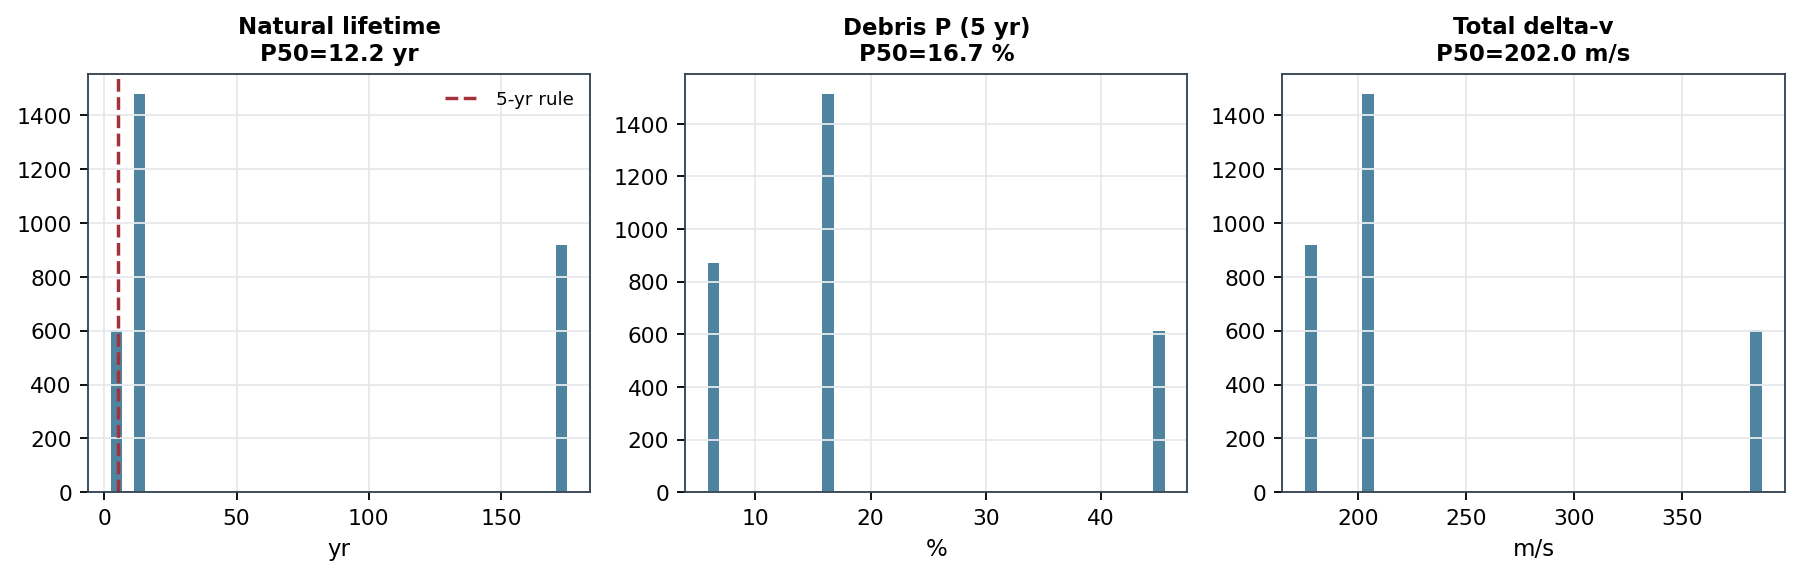
\includegraphics[keepaspectratio,alt={Fig. 19.1, Monte-Carlo distributions of natural lifetime, debris probability, and total Δv across the dominant uncertainties.}]{systems_figs/fig_montecarlo.png}}
\caption{Fig. 19.1, Monte-Carlo distributions of natural lifetime,
debris probability, and total Δv across the dominant uncertainties.}
\end{figure}

\textbf{Derivation of the linear-propagation formula.} Equation (19.1)
follows from a first-order Taylor expansion of the output about the
input means \(\bar{x}=(\bar{x}_1,\dots,\bar{x}_m)\). Writing
\(\delta x_j = x_j-\bar{x}_j\),

\begin{equation}
y \approx f(\bar{x}) + \sum_{j=1}^{m}\frac{\partial f}{\partial x_j}\bigg|_{\bar{x}}\,\delta x_j. \tag{19.2}
\end{equation}

The mean of \(y\) is \(f(\bar{x})\) to this order, so the deviation is
the sum on the right. Forming the variance and using
\(\mathrm{Var}(y)=\mathbb{E}[(y-\bar{y})^2]\) gives, for the general
correlated case,

\begin{equation}
\sigma_y^2 \approx \sum_{j=1}^{m}\sum_{k=1}^{m}\frac{\partial f}{\partial x_j}\frac{\partial f}{\partial x_k}\,\mathrm{Cov}(x_j,x_k). \tag{19.3}
\end{equation}

When the inputs are independent, the cross terms vanish because
\(\mathrm{Cov}(x_j,x_k)=\sigma_{x_j}^2\,\delta_{jk}\), and (19.3)
collapses to (19.1). This makes explicit that (19.1) is the
independent-input special case, and that correlated inputs require the
full covariance sum.

\textbf{Relative-error form for products.} Many of the chapter's outputs
are products and quotients of inputs, for example a flux multiplied by
an area and a time. For a pure power-law monomial
\(y = c\,\prod_j x_j^{a_j}\), the partial derivative is
\(\partial y/\partial x_j = a_j\,y/x_j\), so substitution into (19.1)
yields a clean relative-error rule,

\begin{equation}
\left(\frac{\sigma_y}{y}\right)^2 \approx \sum_{j=1}^{m} a_j^2\left(\frac{\sigma_{x_j}}{x_j}\right)^2. \tag{19.4}
\end{equation}

Each fractional input uncertainty enters weighted by the square of its
exponent, so a variable that appears linearly (\(a_j=1\)) contributes
its fractional spread directly, while one entering quadratically
contributes twice as strongly.

\textbf{Worked example.} Take the catastrophic-impact probability as a
product of debris flux and exposed area over the mission, all with
exponent unity. With the chip-power band of 150 to 200 watts, the
symmetric fractional spread about the 175-watt midpoint is
\(25/175 \approx 0.143\). If a second independent input carries a
comparable \(0.143\) fractional spread, then by (19.4) the output
fractional uncertainty is \(\sqrt{0.143^2 + 0.143^2} \approx 0.20\),
about twenty percent, before the lognormal density term is added by
sampling.

\textbf{Design implication.} Because uncertainties add in quadrature,
the output band is set almost entirely by the one or two widest inputs;
tightening the dominant solar-activity and utilization terms narrows the
headline bands far more than refining any well-known parameter.

\chapter{20. Results: Reference Design Point and
Constellation}\label{results-reference-design-point-and-constellation}

\begin{quote}
\emph{Abstract.} This chapter collects the reference design-point and
constellation results, the numbers that the rest of the book derives and
the open model reproduces.
\end{quote}

Bringing the chapters together, the reference design point and its key
results are summarized in Table 20.1 and the supporting figures.

{\def\LTcaptype{none} % do not increment counter
\begin{longtable}[]{@{}
  >{\raggedright\arraybackslash}p{(\linewidth - 4\tabcolsep) * \real{0.3333}}
  >{\raggedright\arraybackslash}p{(\linewidth - 4\tabcolsep) * \real{0.3333}}
  >{\raggedright\arraybackslash}p{(\linewidth - 4\tabcolsep) * \real{0.3333}}@{}}
\toprule\noalign{}
\begin{minipage}[b]{\linewidth}\raggedright
Quantity
\end{minipage} & \begin{minipage}[b]{\linewidth}\raggedright
Result
\end{minipage} & \begin{minipage}[b]{\linewidth}\raggedright
Driver / chapter
\end{minipage} \\
\midrule\noalign{}
\endhead
\bottomrule\noalign{}
\endlastfoot
Orbital period & 97.6 min & Ch. 4 \\
Natural lifetime (moderate solar) & \textasciitilde22 yr & Ch. 7, fails
5-yr rule \\
Radiator area (1 MW, 20 C) & \textasciitilde1,508 m² & Ch. 10 \\
Interface ΔT (700 W chip) & 210 C (\textgreater125 budget) & Ch. 10,
active cooling needed \\
5-yr dose behind 10 mm Al & \textasciitilde1.06 krad(Si) & Ch. 8, large
margin \\
Catastrophic debris P (cluster, 5 yr) & \textasciitilde17\% (6-46\%
band) & Ch. 9 \\
In-cluster cascade P (neighbor, 150 m) & \textasciitilde8.5\% & Ch. 13 /
risk synthesis \\
De-orbit Δv & 131.6 m/s (of \textasciitilde190 total) & Ch. 15 \\
Passive H100 throttle loss & \textasciitilde90\% & Ch. 17 \\
Reference dry mass & \textasciitilde270-290 kg & Ch. 12, 18 \\
\end{longtable}
}

The debris and radiation results, central to the survivability case, are
shown in Figs. 20.1 and 20.2. The debris figure shows both the
cluster-level catastrophic probability over the mission and the
in-cluster cascade coupling versus formation spacing; the radiation
figure shows the dose-versus-shielding curve against the memory
tolerance and the reliability-versus-throughput trade.

\begin{figure}
\centering
\pandocbounded{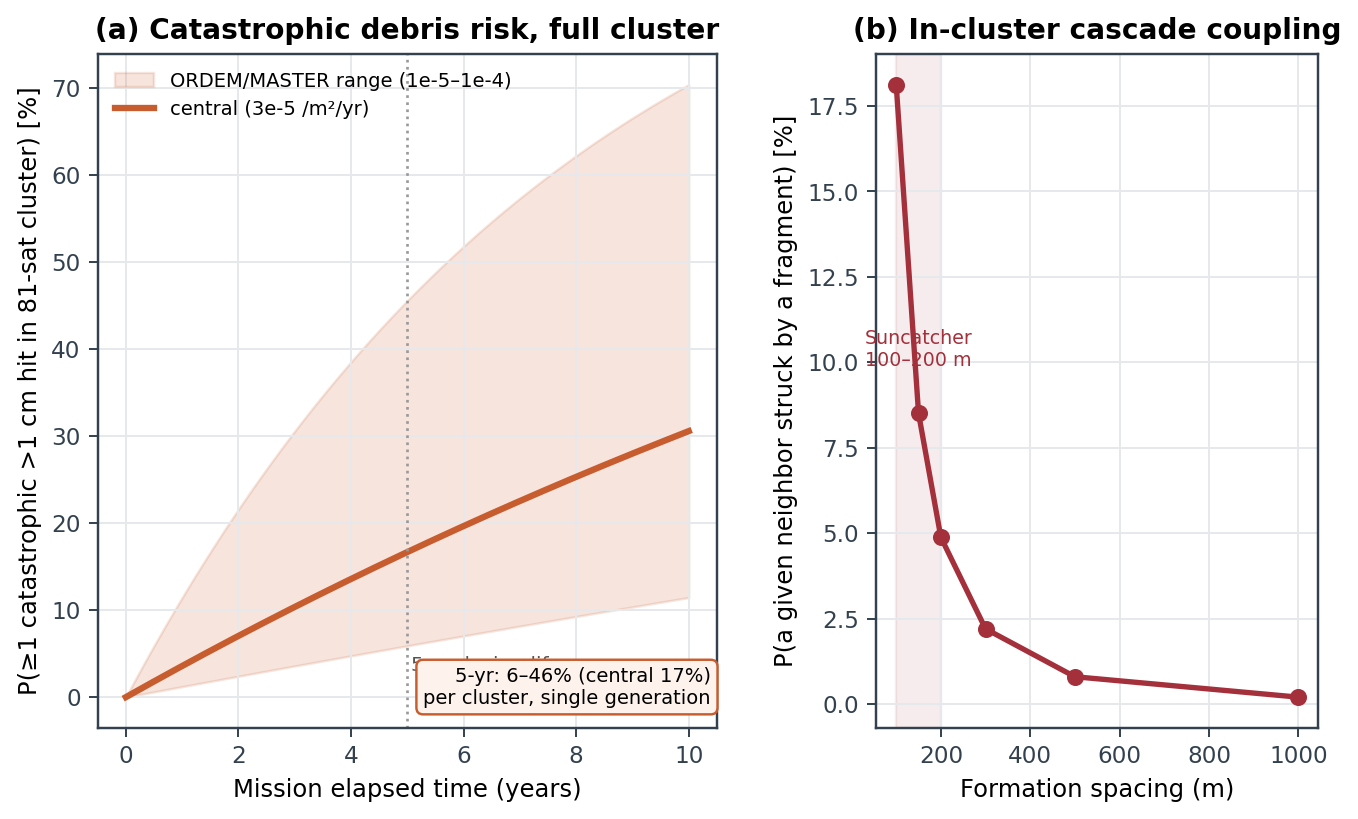
\includegraphics[keepaspectratio,alt={Fig. 20.1, Catastrophic debris risk for the full cluster, and the in-cluster cascade coupling versus formation spacing.}]{figures/fig3_debris_risk.png}}
\caption{Fig. 20.1, Catastrophic debris risk for the full cluster, and
the in-cluster cascade coupling versus formation spacing.}
\end{figure}

\begin{figure}
\centering
\pandocbounded{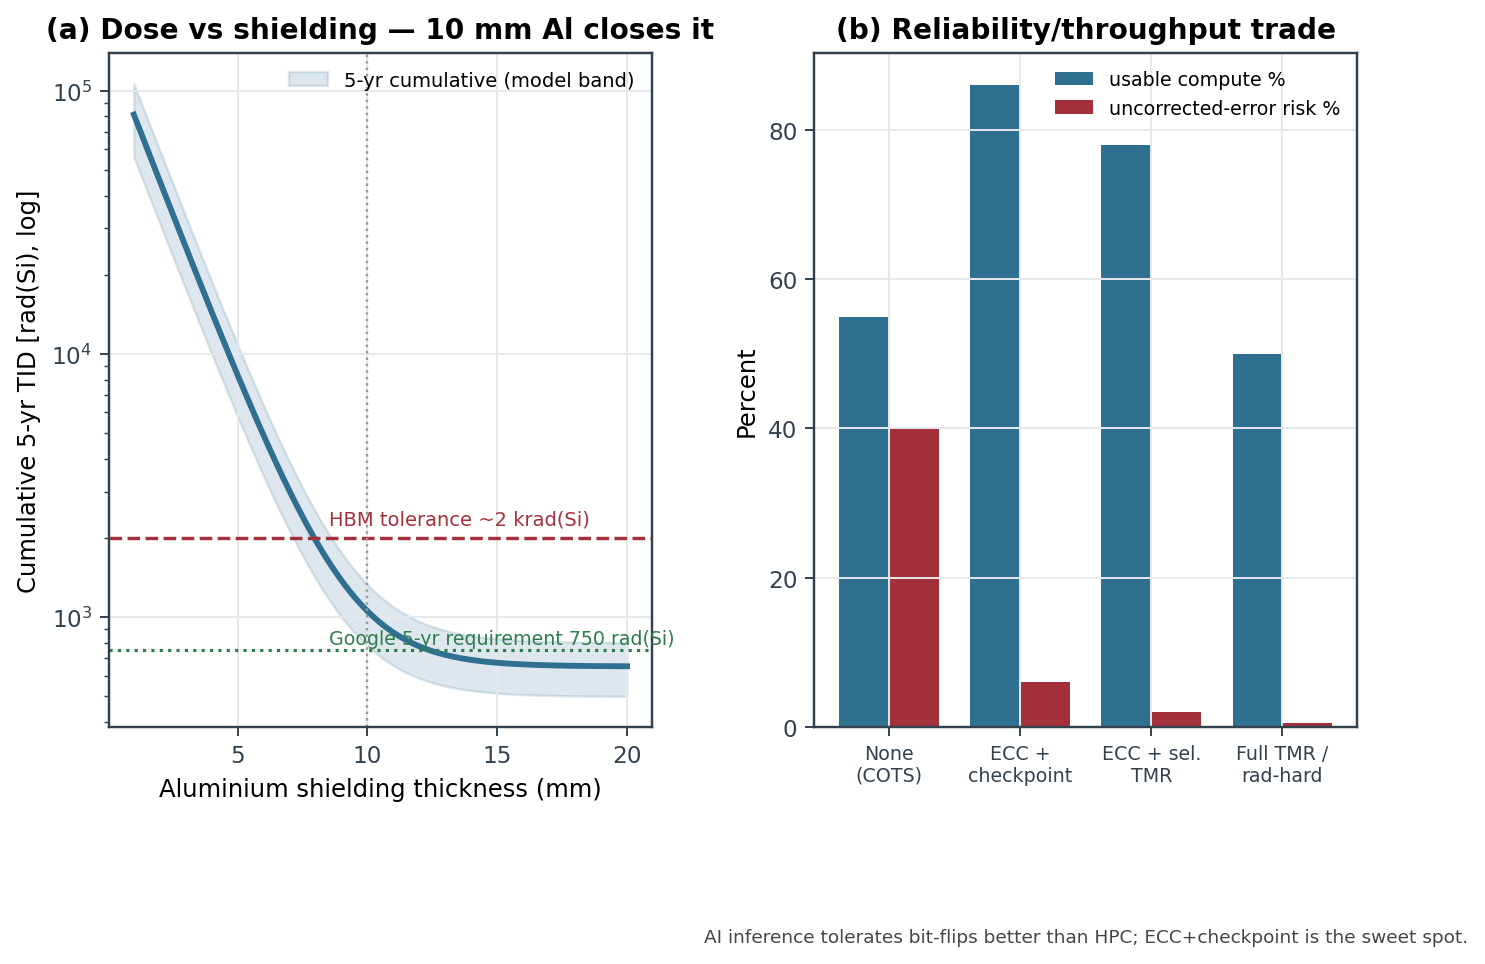
\includegraphics[keepaspectratio,alt={Fig. 20.2, Cumulative dose versus aluminium shielding, and the reliability-throughput trade.}]{figures/fig4_radiation.png}}
\caption{Fig. 20.2, Cumulative dose versus aluminium shielding, and the
reliability-throughput trade.}
\end{figure}

\begin{center}\rule{0.5\linewidth}{0.5pt}\end{center}

\textbf{From orbital period to the survivability clock.} The reference
period in Table 20.1 follows directly from Kepler's third law for a
near-circular orbit. With \(\mu\) the standard gravitational parameter
of Earth, \(R_\oplus\) the mean radius, and \(h\) the orbital altitude,
the semi-major axis is \(a = R_\oplus + h\) and the period is

\begin{equation}
T = 2\pi \sqrt{\frac{a^{3}}{\mu}} = 2\pi \sqrt{\frac{(R_\oplus + h)^{3}}{\mu}}. \tag{20.1}
\end{equation}

Differentiating gives the sensitivity of the period to altitude, which
sets how tightly a constellation must hold its altitude band before its
members drift in phase:

\begin{equation}
\frac{dT}{dh} = \frac{3\pi}{\sqrt{\mu}}\,\sqrt{R_\oplus + h}. \tag{20.2}
\end{equation}

The orbital mean motion \(n = 2\pi / T\) then fixes the revisit and
eclipse cadence that the thermal and power budgets of the preceding
chapters are built upon.

\textbf{Why the lifetime fails the five-year rule.} The natural-lifetime
entry is governed by atmospheric drag removing orbital energy. For a
circular orbit the specific energy is \(\varepsilon = -\mu / (2a)\), so
a small decay in semi-major axis costs energy at the rate

\begin{equation}
\frac{d\varepsilon}{dt} = \frac{\mu}{2 a^{2}}\,\frac{da}{dt}, \tag{20.3}
\end{equation}

and the drag force on a body of mass \(m\), cross-section \(A\), and
drag coefficient \(C_D\) in atmospheric density \(\rho\) moving at
\(v = \sqrt{\mu / a}\) does work at the rate that drains this energy.
Balancing the two yields the decay rate of the semi-major axis,

\begin{equation}
\frac{da}{dt} = -\,C_D\,\frac{A}{m}\,\rho\, \sqrt{\mu\, a}. \tag{20.4}
\end{equation}

The grouping \(A/m\) is the area-to-mass ratio, the single most
important design variable here. A compact dry mass of roughly 270 to 290
kg, as listed in Table 20.1, drives \(A/m\) low, which lengthens the
lifetime toward the cited 22 years and is precisely why the design fails
the 5-year passive-disposal rule and must carry the de-orbit budget of
Chapter 15.

\textbf{Worked example, debris-risk scaling.} The catastrophic-collision
probability over a mission accumulates as a Poisson process with hazard
rate proportional to the swept cross-section. If a single satellite
carries probability \(p_1\), then for a cluster of \(N\) effectively
independent members the cluster-level probability is

\begin{equation}
P_{\mathrm{cluster}} = 1 - (1 - p_1)^{N}. \tag{20.5}
\end{equation}

For small \(p_1\) this is close to \(N p_1\). The cluster figure of
about 17 percent is therefore dominated by member count, so adding
satellites raises survivability cost super-linearly. The design
implication is direct: constellation sizing cannot be separated from the
per-member debris hazard, and growth in \(N\) must be paid for in either
shielding mass or accepted mission risk.

\part{ECONOMICS AND PREDICTIONS}\label{economics-and-predictions}

\chapter{21. Techno-Economics: Cost, NPV, and the Levelized Cost of
Compute}\label{techno-economics-cost-npv-and-the-levelized-cost-of-compute}

\begin{quote}
\emph{Abstract.} This chapter develops the techno-economics, capital and
operating cost, net present value, and the levelized cost of useful
compute.
\end{quote}

\emph{Sources: the levelized-cost and net-present-value formulation
follows standard engineering economics and the SMAD cost treatment
{[}18{]}; launch-cost inputs per {[}35{]} and the reference architecture
{[}1{]}.}

The economic case is built with a proper time-value-of-money treatment
rather than simple cost bookkeeping.

\textbf{Cost structure and the launch cross-over.} Per-satellite cost is
launch plus hardware,
\(C_{\mathrm{sat}} = p_{\mathrm{launch}}\, m_{\mathrm{launch}} + C_{\mathrm{hw}}\).
Launch equals hardware at the cross-over price
\(p^{*} = C_{\mathrm{hw}}/m_{\mathrm{launch}}\); with about 1.1 million
dollars of hardware on a 415-kg satellite,
\(p^{*} \approx 2{,}650\ \mathrm{USD/kg}\). Below this price, hardware
dominates, and below roughly 600 USD/kg the launch term is a small
correction. The economics are therefore gated by hardware cost,
lifetime, utilization, and the radiation tax, not by the headline
dollar-per-kilogram figure that dominates public discussion.

\textbf{Discounted cash flow.} The capital-recovery factor that
annualizes a capital cost over \(n\) years at discount rate \(r\) is
\(\mathrm{CRF} = r(1+r)^n/[(1+r)^n - 1]\). Net present value is
\(\mathrm{NPV} = \sum_t \mathrm{CF}_t/(1+r)^t\), and the internal rate
of return is the rate at which NPV vanishes, solved by bisection.

\textbf{Levelized cost of compute.} The most decision-relevant metric is
the levelized cost per useful petaflop-hour:

\begin{equation}
\mathrm{LCOE} = \frac{\mathrm{CRF}\cdot \mathrm{CAPEX} + \mathrm{OPEX}_{\mathrm{yr}}}
{\text{annual useful PFLOP-hours}}. \tag{21.1}
\end{equation}

Because the denominator uses delivered, throttled,
utilization-and-availability-derated compute, a high-power chip that
throttles under passive cooling shows a dramatically worse levelized
cost than its peak rating implies, quantifying, in dollars, the penalty
of the interface wall. Replenishment, at the reliability-driven rate of
Chapter 16, is a first-order operating expense in this calculation.

\begin{figure}
\centering
\pandocbounded{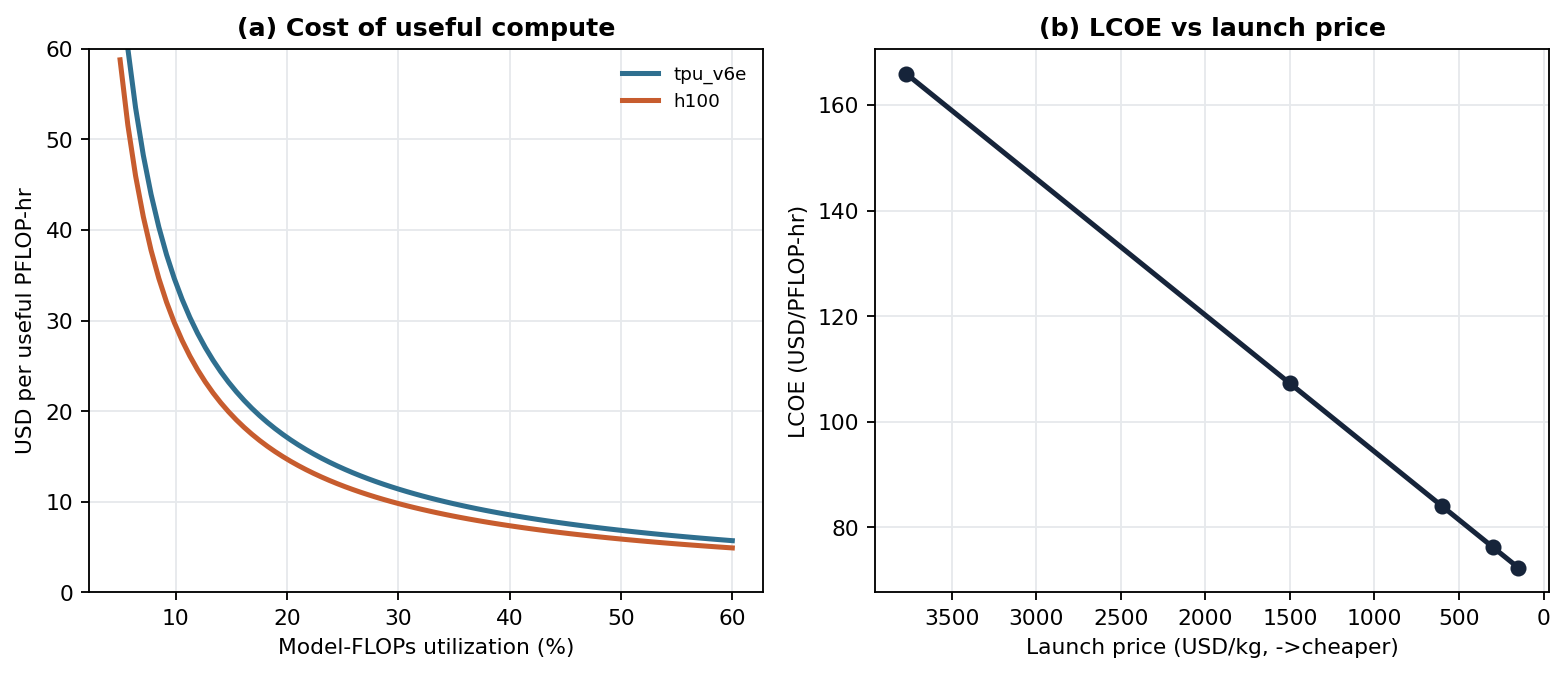
\includegraphics[keepaspectratio,alt={Fig. 21.1b Levelized cost of useful compute versus model-FLOPs utilization, and versus launch price. The cost is dominated by utilization and hardware, not by launch.}]{figures2/figA7_lcoe.png}}
\caption{Fig. 21.1b Levelized cost of useful compute versus model-FLOPs
utilization, and versus launch price. The cost is dominated by
utilization and hardware, not by launch.}
\end{figure}

\begin{figure}
\centering
\pandocbounded{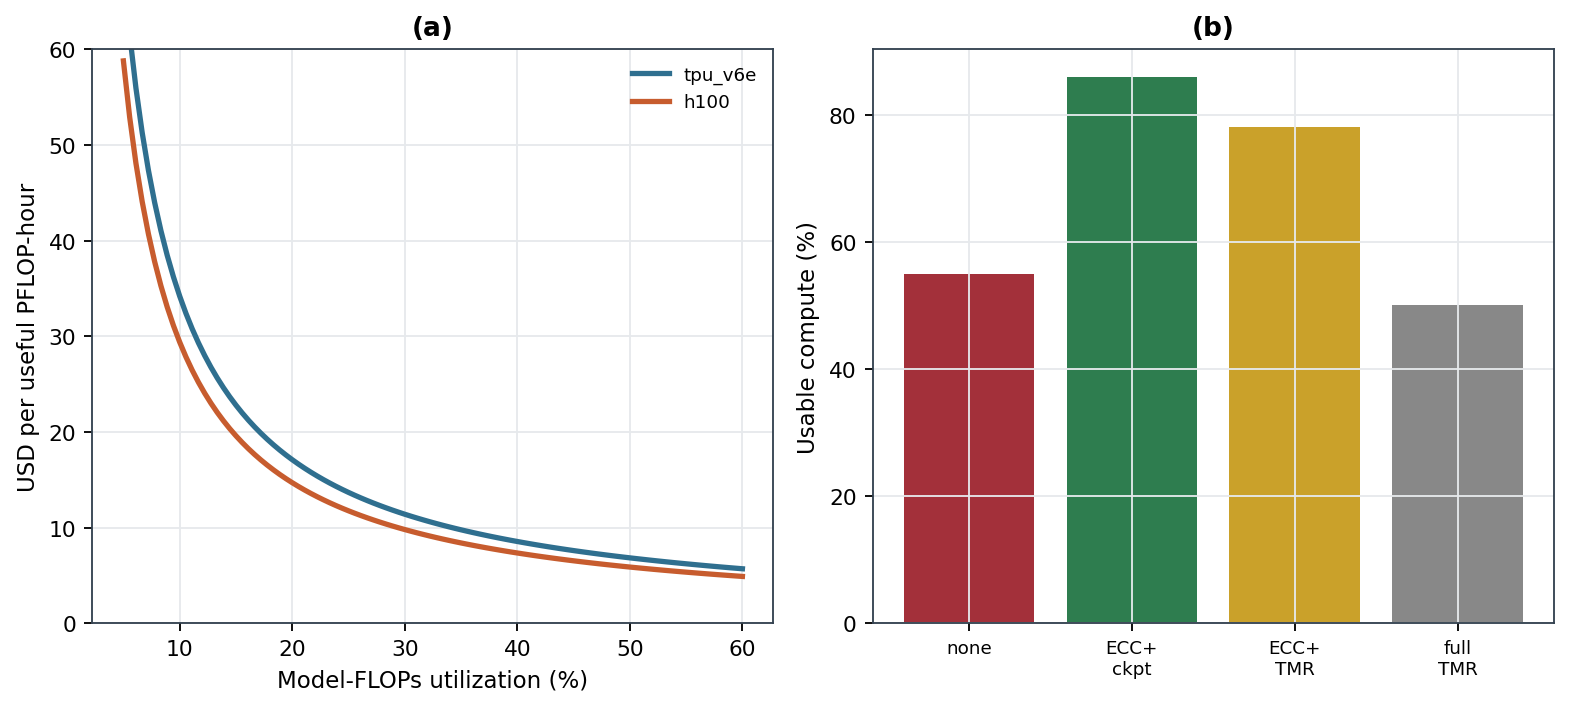
\includegraphics[keepaspectratio,alt={Fig. 21.1, Cost of useful compute versus utilization, and the radiation throughput tax by protection level.}]{systems_figs/fig_compute.png}}
\caption{Fig. 21.1, Cost of useful compute versus utilization, and the
radiation throughput tax by protection level.}
\end{figure}

\textbf{Deriving the launch cross-over price.} The per-satellite cost
separates into a launch term that scales with delivered mass and a fixed
hardware term,

\begin{equation}
C_{\mathrm{sat}} = p_{\mathrm{launch}}\, m_{\mathrm{launch}} + C_{\mathrm{hw}}. \tag{21.2}
\end{equation}

The two contributions are equal when
\(p_{\mathrm{launch}}\, m_{\mathrm{launch}} = C_{\mathrm{hw}}\). Solving
for the price isolates the cross-over,

\begin{equation}
p^{*} = \frac{C_{\mathrm{hw}}}{m_{\mathrm{launch}}}. \tag{21.3}
\end{equation}

With the chapter's reference values,
\(C_{\mathrm{hw}} \approx 1.1\times 10^{6}\ \mathrm{USD}\) and
\(m_{\mathrm{launch}} = 415\ \mathrm{kg}\), the cross-over evaluates to
\(p^{*} = 1.1\times 10^{6}/415 \approx 2{,}650\ \mathrm{USD/kg}\),
consistent with the figure quoted in the body. The derivative
\(\partial C_{\mathrm{sat}}/\partial p_{\mathrm{launch}} = m_{\mathrm{launch}}\)
is constant, so once \(p_{\mathrm{launch}} \ll p^{*}\) the satellite
cost flattens onto the hardware floor and further reductions in launch
price return little.

\textbf{The capital-recovery factor as a geometric sum.} Annualizing a
capital cost requires the level payment \(A\) whose discounted stream
over \(n\) years equals the principal. Writing the present value of
\(n\) equal payments and summing the geometric series gives

\begin{equation}
\mathrm{CAPEX} = A\sum_{t=1}^{n}\frac{1}{(1+r)^{t}} = A\,\frac{1-(1+r)^{-n}}{r}, \tag{21.4}
\end{equation}

and inverting for the annuity per unit principal yields the
capital-recovery factor used in (21.1),

\begin{equation}
\mathrm{CRF} = \frac{A}{\mathrm{CAPEX}} = \frac{r\,(1+r)^{n}}{(1+r)^{n}-1}. \tag{21.5}
\end{equation}

In the limit \(r\to 0\) the factor reduces to \(\mathrm{CRF}\to 1/n\),
recovering straight-line amortization; for \(r>0\) it exceeds \(1/n\),
charging the project for the time value of locked capital.

\textbf{Useful compute and the utilization chain.} The denominator of
(21.1) is the peak rating successively derated by the model-FLOPs
utilization \(u\), the operational availability \(A_{\mathrm{op}}\), and
the throttling factor \(\eta_{\mathrm{th}}\) set by the thermal
interface,

\begin{equation}
\text{PFLOP-hours}_{\mathrm{yr}} = P_{\mathrm{peak}}\,\eta_{\mathrm{th}}\,u\,A_{\mathrm{op}}\,(8760\ \mathrm{h}). \tag{21.6}
\end{equation}

Because
\(\mathrm{LCOE}\propto 1/(\eta_{\mathrm{th}}\,u\,A_{\mathrm{op}})\), the
levelized cost is hyperbolic in each derating term; a chip that
throttles to \(\eta_{\mathrm{th}}=0.5\) doubles the cost of every
delivered petaflop-hour regardless of its peak specification.

\textbf{Design implication.} The economics are governed by hardware
cost, lifetime, and the multiplicative utilization chain rather than by
the headline launch price, so design effort returns more when spent
raising sustained utilization and availability than when spent chasing
marginal dollar-per-kilogram gains below the cross-over.

\chapter{22. The Launch-Cost-Parity
Prediction}\label{the-launch-cost-parity-prediction}

\begin{quote}
\emph{Abstract.} This chapter tests the launch-cost-parity assumption
that underwrites the business case, and finds that most sampled futures
never reach the target price within the horizon, with parity, where it
arrives, falling later than the headline date.
\end{quote}

\emph{Sources: the learning-curve and cadence inputs follow the
reference architecture's cost model {[}1{]} and public launch data
{[}35{]}.}

The entire economic case rests on launch cost falling far enough that
the annualized cost of power in orbit approaches the terrestrial cost of
power. The reference paper projects launch reaching 200 dollars per
kilogram by about 2035 under a twenty-percent learning rate, requiring
on the order of 370,000 tonnes of additional cumulative launched mass,
some 1,800 Starship launches, at which point the launched-power price of
roughly 810 dollars per kilowatt-year approaches the terrestrial
data-center power spend of 570 to 3,000 dollars per kilowatt-year. The
broader launch-cost landscape that frames this target is shown in Fig.
22.1: today's reusable launch still sits an order of magnitude above it,
and once the price falls below roughly 600 dollars per kilogram the
all-in cost per satellite is set by hardware rather than launch, so
further reductions in launch price yield diminishing returns.

\begin{figure}
\centering
\pandocbounded{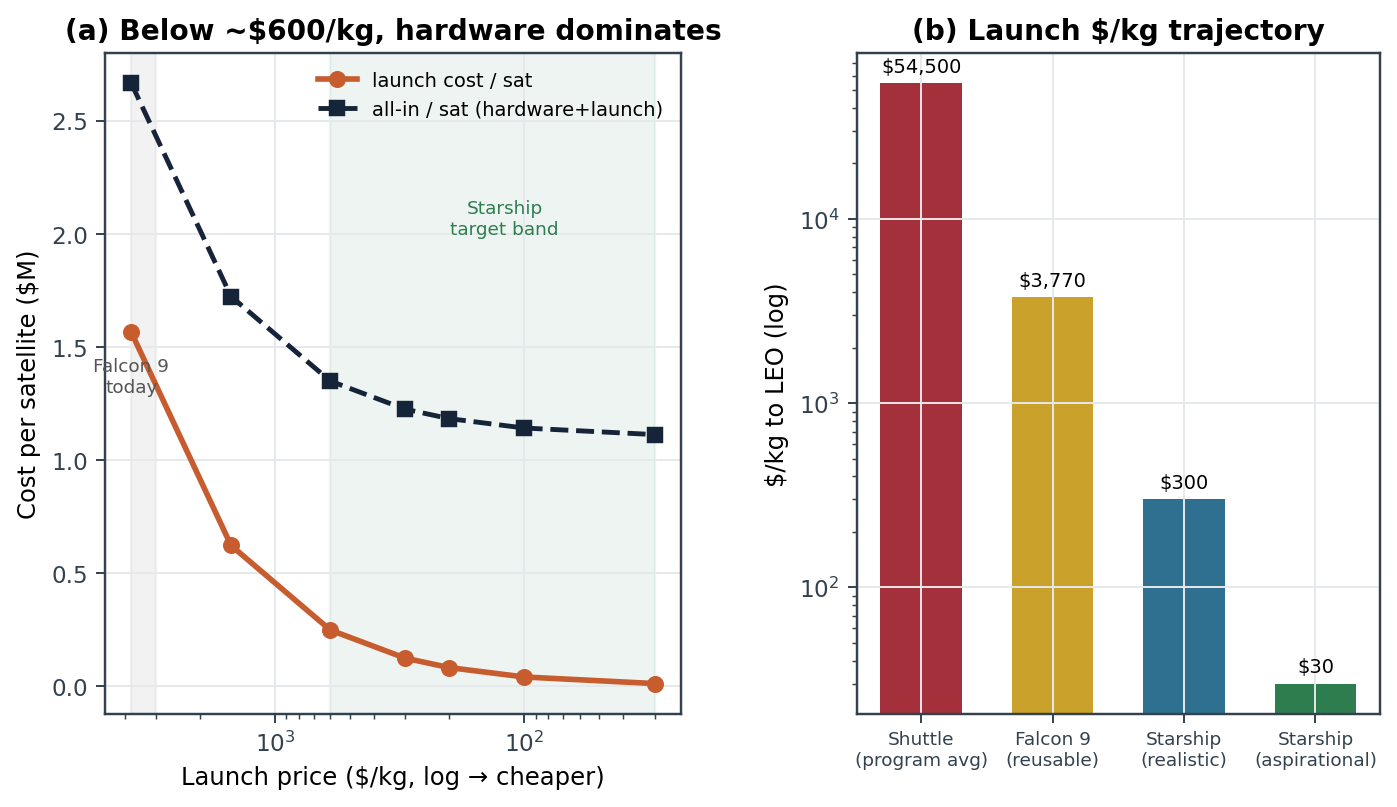
\includegraphics[keepaspectratio,alt={Fig. 22.1. The launch-cost landscape. Left: below roughly 600 dollars per kilogram the all-in cost per satellite is dominated by hardware rather than launch. Right: the price-per-kilogram trajectory to low Earth orbit, from the Shuttle program average through reusable Falcon 9 to the realistic and aspirational Starship targets.}]{figures/fig6_launch_cost.png}}
\caption{Fig. 22.1. The launch-cost landscape. Left: below roughly 600
dollars per kilogram the all-in cost per satellite is dominated by
hardware rather than launch. Right: the price-per-kilogram trajectory to
low Earth orbit, from the Shuttle program average through reusable
Falcon 9 to the realistic and aspirational Starship targets.}
\end{figure}

This forecast is assumption-fragile, so this study generates its own
credibility band rather than inheriting a single date. A Wright learning
curve is applied to cumulative launched mass, with a logistic ramp in
launch cadence, and the unproven assumptions are sampled by Monte-Carlo:
the learning rate from fifteen to twenty-five percent, the 2026
effective price from 1,200 to 3,500 dollars per kilogram, the payload
from 150 to 250 tonnes, and the peak cadence from 80 to 220 launches per
year. The first result is the more important one and is easy to miss in
a single headline date: across the sampled assumptions, only about five
percent of scenarios reach 200 dollars per kilogram at all within the
2050 horizon, and roughly ninety-five percent never reach it. Parity at
that price is therefore not a near-certainty awaiting a date; under most
defensible assumptions it does not arrive within the horizon.
Conditional on the minority of scenarios that do reach it, the median
parity year is near 2044 (Fig. 22.1), with a fifth percentile of about
2037 and essentially no probability of reaching parity by 2035.
Extending the horizon to 2060 raises the reaching fraction only to about
nine percent and moves the conditional median to the end of the 2040s,
so the conclusion is not an artifact of where the horizon is drawn. The
vendor's 2035 date sits beyond the optimistic edge of the distribution
and requires its specific aggressive anchors, full reusability at 200
tonnes and roughly two million dollars marginal cost, sustained
twenty-percent learning from a low starting price, and a total launched
mass far larger than the cadence ranges sampled here deliver.

The prediction is therefore twofold: launch-cost parity at 200 dollars
per kilogram is unlikely under most assumptions rather than merely late,
and where it does arrive it is more likely in the late 2030s to
mid-2040s than in 2035. Parity is in any case necessary but not
sufficient: even at parity, the business case is gated by hardware cost,
lifetime, and utilization.

\begin{figure}
\centering
\pandocbounded{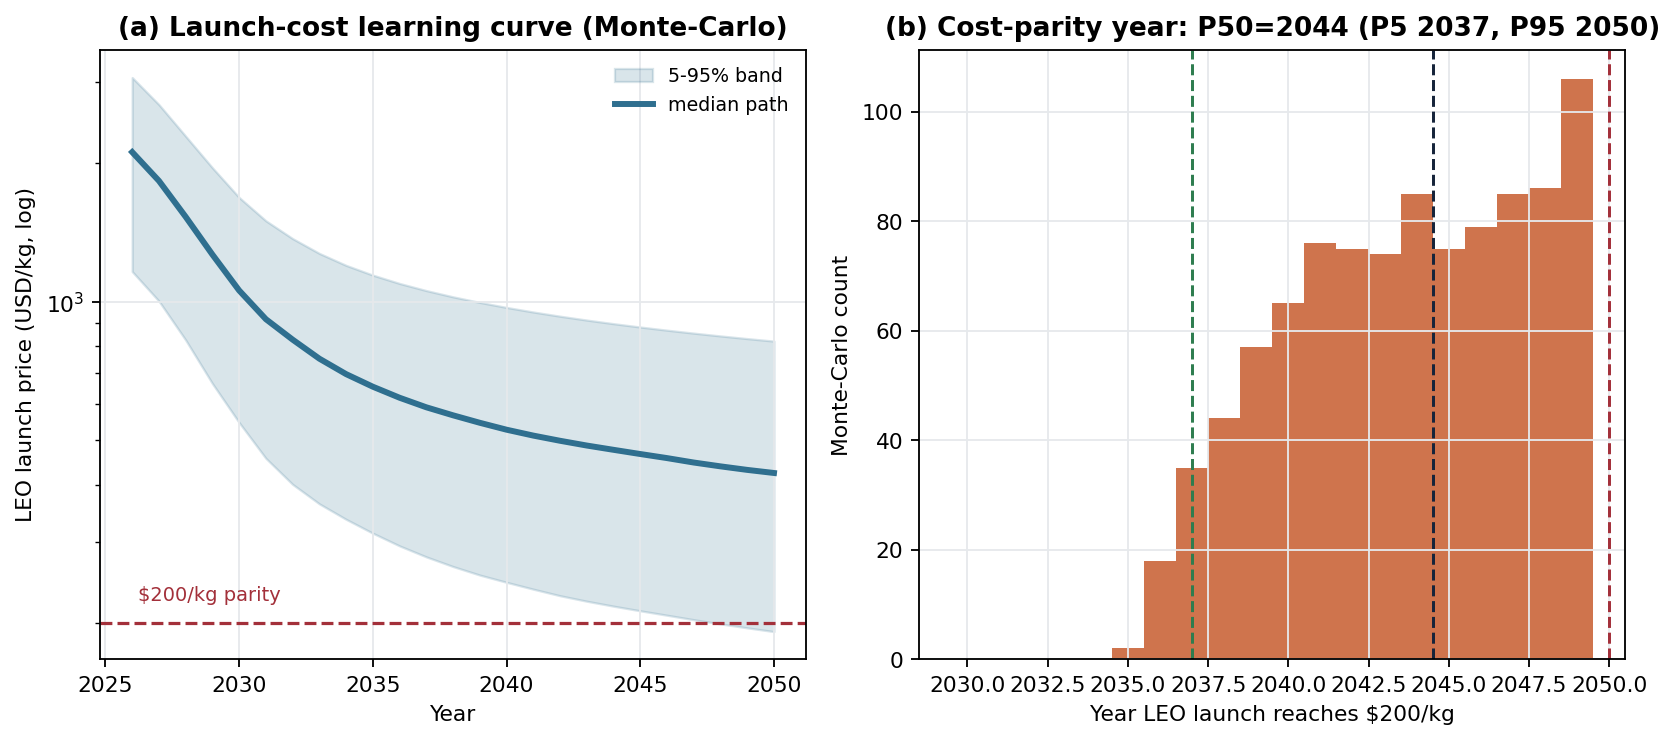
\includegraphics[keepaspectratio,alt={Fig. 22.2, Launch-cost learning curve (Monte-Carlo) and the distribution of the cost-parity year. Most sampled scenarios never reach 200 dollars per kilogram within the horizon; conditional on those that do, the median is near 2044, later than the vendor's 2035.}]{figures_pred/fig_cost_parity.png}}
\caption{Fig. 22.2, Launch-cost learning curve (Monte-Carlo) and the
distribution of the cost-parity year. Most sampled scenarios never reach
200 dollars per kilogram within the horizon; conditional on those that
do, the median is near 2044, later than the vendor's 2035.}
\end{figure}

\textbf{The Wright learning curve in detail.} The cost model rests on a
Wright relation, in which the unit price of launch falls by a constant
fraction for every doubling of cumulative launched mass. If \(C(m)\) is
the effective price per kilogram at cumulative launched mass \(m\), and
\(C_0\) is the price at a reference mass \(m_0\), the relation is

\begin{equation}
C(m) = C_0 \left( \frac{m}{m_0} \right)^{-b}, \tag{22.1}
\end{equation}

where the exponent \(b\) encodes the learning rate. The learning rate
\(L\) is defined as the fractional reduction per doubling, so that two
successive doublings satisfy \(C(2m)/C(m) = 1 - L\). Substituting
\(m \to 2m\) into (22.1) gives \(C(2m)/C(m) = 2^{-b}\), and equating the
two expressions yields

\begin{equation}
2^{-b} = 1 - L, \qquad b = -\frac{\ln(1 - L)}{\ln 2}. \tag{22.2}
\end{equation}

A twenty-percent learning rate, \(L = 0.20\), therefore corresponds to
\(b = -\ln(0.80)/\ln 2 \approx 0.322\).

\textbf{Solving for the mass required to hit a target price.} The design
question is inverted from (22.1): given a target price \(C^\ast\), how
much cumulative mass must be launched? Setting \(C(m) = C^\ast\) and
rearranging,

\begin{equation}
\frac{m}{m_0} = \left( \frac{C^\ast}{C_0} \right)^{-1/b}, \tag{22.3}
\end{equation}

so the required cumulative mass grows as a steep inverse power of the
target price. With a target of 200 dollars per kilogram, the small ratio
\(C^\ast/C_0\) is amplified by the exponent \(1/b \approx 3.1\), which
is why the model calls for cumulative launched mass on the order of
hundreds of thousands of tonnes.

\textbf{The cadence ramp and the parity year.} Cumulative mass accrues
over time through flights. With a logistic ramp in annual cadence
approaching a peak rate, the cumulative mass at time \(t\) is the
integral of payload times cadence,

\begin{equation}
m(t) = m_0 + p \int_{t_0}^{t} R(\tau)\, d\tau, \tag{22.4}
\end{equation}

where \(p\) is payload per launch and \(R(\tau)\) is the
launches-per-year ramp. The parity year \(t^\ast\) is the time at which
\(m(t^\ast)\) first equals the mass required by (22.3); combining (22.3)
and (22.4) shows that \(t^\ast\) depends jointly on the learning
exponent, the starting price, the payload, and the integrated cadence,
which is why sampling these four inputs spreads parity across a wide
band rather than fixing a single date.

\textbf{Worked estimate.} Take \(L = 0.20\), so \(b \approx 0.322\) and
\(1/b \approx 3.1\). If the effective price must fall by roughly a
factor of ten to approach the target, then from (22.3) the cumulative
mass must rise by a factor of about \(10^{3.1} \approx 1.3 \times 10^3\)
over its reference value, which at a payload near 200 tonnes per flight
calls for many hundreds of flights even before the slower logistic tail.

\textbf{Design implication.} Because required mass scales as the target
price raised to the power \(-1/b\), the parity date is acutely sensitive
to the learning rate and the starting price; a planner should treat
parity as a distribution conditioned on those inputs, not a fixed
milestone, and should not commit capital on the assumption that the
headline date will arrive.

\chapter{23. Capability and Risk Trajectory,
2027-2035}\label{capability-and-risk-trajectory-2027-2035}

\begin{quote}
\emph{Abstract.} This chapter synthesizes the preceding analysis into a
defensible capability and risk trajectory through the early 2030s, and
names the gating demonstrations.
\end{quote}

\begin{figure}
\centering
\pandocbounded{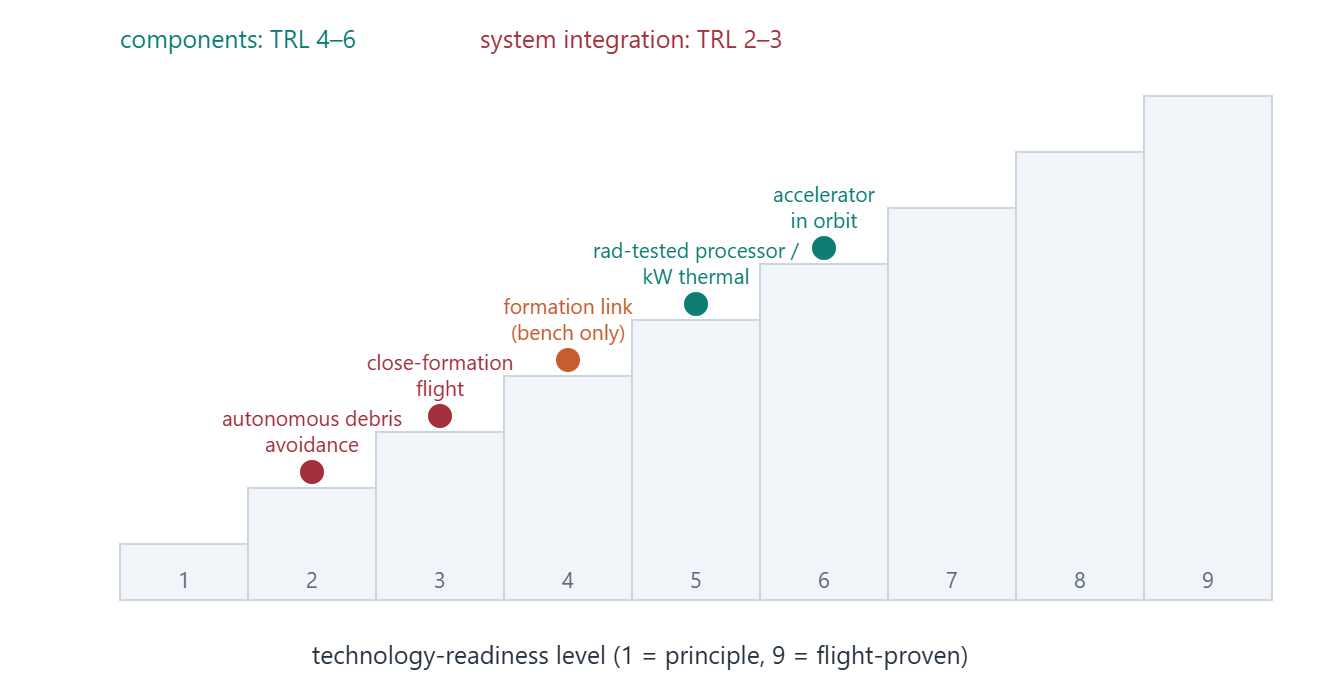
\includegraphics[keepaspectratio,alt={Technology-readiness ladder: the components sit mid-scale, while system integration sits near the bottom.}]{schematics/diagram_trl.png}}
\caption{Technology-readiness ladder: the components sit mid-scale,
while system integration sits near the bottom.}
\end{figure}

Synthesizing the technology-readiness picture of Chapter 2 with the
engineering constraints of the preceding chapters yields a defensible
capability trajectory. By 2027, the demonstration missions (the
Suncatcher two-satellite prototype, Starcloud's Blackwell-class
follow-on) should place real accelerators in orbit and exercise
components, raising their readiness while leaving constellation-scale
operation unproven. Through 2028 to 2030, the gating demonstrations are
flown multi-terabit formation links, validated formation station-keeping
under the differential drag of the solar cycle, and, most importantly,
autonomous, cluster-coordinated debris avoidance at sub-kilometer
spacing. From 2030 to 2035, if launch trends hold, niche economic cases
emerge for latency-critical or space-native workloads, while gigawatt
scale remains aspirational and cost parity, per Chapter 22, is unlikely
before the mid-2030s.

The debris-and-Kessler trajectory deserves particular attention: a
one-kilometer cluster in the congested 650-km shell raises both the
catastrophic-impact exposure and the cascade hazard, and its evolution
depends on disposal compliance and avoidance autonomy. A flight program
should quantify this with the official ORDEM 3.2 and LEGEND tools before
committing to constellation scale.

\begin{center}\rule{0.5\linewidth}{0.5pt}\end{center}

\textbf{From component readiness to system readiness.} The chapter
treats the readiness ladder qualitatively, with components mid-scale and
integration near the bottom. A useful way to make this precise for a
constellation is to recognize that a serial chain of independently
gating subsystems behaves multiplicatively. If the program must clear
\(n\) gating demonstrations and each demonstration \(i\) has an
independent success probability \(p_i\), then the probability that the
integrated system reaches operational readiness is the product

\begin{equation}
P_{\text{sys}} = \prod_{i=1}^{n} p_i. \tag{23.1}
\end{equation}

Taking logarithms converts the product into a sum that exposes the
weakest link,

\begin{equation}
\ln P_{\text{sys}} = \sum_{i=1}^{n} \ln p_i, \tag{23.2}
\end{equation}

so the demonstration with the smallest \(p_i\) contributes the largest
negative term and dominates the schedule. This is the formal reason the
chapter elevates autonomous, cluster-coordinated debris avoidance above
the link and station-keeping milestones: a single low-probability gate
caps the whole product. For a quick worked figure, the three gating
demonstrations named in the text, formation links, station-keeping under
solar-cycle drag, and avoidance autonomy, with illustrative values
\(p_1 = 0.9\), \(p_2 = 0.8\), \(p_3 = 0.5\), give
\(P_{\text{sys}} = 0.9 \times 0.8 \times 0.5 = 0.36\), confirming that
the autonomy gate sets the ceiling.

\textbf{Cascade exposure in the congested shell.} The debris-and-Kessler
concern can be carried one step further than the prose. For a cluster
presenting collision cross-section \(A\) moving at relative speed
\(v_{\text{rel}}\) through a debris number density \(\rho\), the
expected catastrophic-impact rate is

\begin{equation}
\lambda = \rho\, A\, v_{\text{rel}}, \tag{23.3}
\end{equation}

and over a mission of duration \(T\) the probability of at least one
such impact, assuming Poisson statistics, is

\begin{equation}
P_{\text{hit}} = 1 - e^{-\lambda T}. \tag{23.4}
\end{equation}

Avoidance autonomy enters as a multiplier that suppresses the effective
rate to \(\lambda_{\text{eff}} = (1-\eta)\,\lambda\), where \(\eta\) is
the fraction of conjunctions resolved by maneuver; the cascade hazard
scales with the residual \(\lambda_{\text{eff}}\) together with disposal
compliance. These relations are the analytic skeleton that the official
ORDEM 3.2 and LEGEND tools populate with shell-specific densities.

\textbf{Design implication.} Schedule and capital should be concentrated
on raising the lowest-probability gate, since equations (23.1) and
(23.2) show it bounds system readiness; and avoidance autonomy must be
sized to drive \(\eta\) high enough that the residual rate in equation
(23.3) keeps cascade exposure within the program's risk budget.

\part{SYNTHESIS}\label{synthesis}

\chapter{24. Caveats and Limitations}\label{caveats-and-limitations}

\begin{quote}
\emph{Abstract.} This chapter states plainly what the study does and
does not establish, including the quality of its sources and the model
fidelity it deliberately stops short of.
\end{quote}

A complete assessment must state clearly what this study does and does
not establish.

On source quality: the single most load-bearing source for the
radiation, link-budget, and cost-parity claims is a non-peer-reviewed,
vendor-authored preprint; its results are self-reported and not
independently replicated. On the technology-readiness gap: what has been
demonstrated is one data-center-class GPU in orbit, ground radiation
testing of a TPU, a bench-scale optical link, and kilowatt-class nodes;
what the vision requires, megawatt-to-gigawatt clusters, flown
multi-terabit formation links, dramatically cheaper launch, and
in-flight formation control, has not been demonstrated. On model
fidelity: the debris flux, atmospheric density, and radiative limits
used here are computed at first order with explicit uncertainty bands,
not measured per-orbit; a flight program would use the official agency
tools (NASA DAS, ORDEM 3.2, ESA MASTER and DRAMA, SPENVIS/SHIELDOSE-2)
and a full thermal and orbit toolchain. The model also omits, by design,
a multi-node thermal finite-element analysis, a closed-loop
attitude-control simulation, formal failure-modes and effects analysis,
micrometeoroid Whipple-shield sizing, and a full time-domain mission
simulation. Finally, several widely repeated marketing claims, notably
``ten times cheaper including launch'', failed independent verification
and are not relied upon here.

These limitations do not undermine the study's purpose, which is to size
the problem, rank the risks, and quantify the trades transparently. They
do bound the confidence with which any single number should be quoted,
and they identify exactly where higher-fidelity work is needed next.

\textbf{On compounding the independent uncertainty bands.} The chapter
reports several first-order quantities, each carrying an explicit
uncertainty band rather than a measured value. When a derived figure of
merit depends on more than one of these quantities, the bands must be
combined rather than quoted singly. For a quantity \(Q\) that is a
product of independent inputs \(x_i\),

\[ Q = \prod_{i=1}^{n} x_i^{\,a_i}, \]

the relative uncertainty follows from logarithmic differentiation.
Taking logarithms gives \(\ln Q = \sum_i a_i \ln x_i\), and
differentiating yields
\(\mathrm{d}Q/Q = \sum_i a_i\,\mathrm{d}x_i/x_i\). Treating the inputs
as independent and adding their variances in quadrature gives

\begin{equation}
\left(\frac{\sigma_Q}{Q}\right)^{2} = \sum_{i=1}^{n} a_i^{2}\left(\frac{\sigma_{x_i}}{x_i}\right)^{2}. \tag{24.1}
\end{equation}

This relation explains why any single number derived from the model
carries a wider band than its individual inputs, and why a low-fidelity
quantity propagates into every figure of merit that uses it.

\textbf{On the dominance of the worst input.} Equation (24.1) shows that
the term with the largest \(|a_i|\,\sigma_{x_i}/x_i\) governs the total.
If one input dominates so strongly that
\(a_k^2(\sigma_{x_k}/x_k)^2 \gg \sum_{i\neq k} a_i^2(\sigma_{x_i}/x_i)^2\),
then

\begin{equation}
\frac{\sigma_Q}{Q} \;\approx\; \left|a_k\right|\frac{\sigma_{x_k}}{x_k}. \tag{24.2}
\end{equation}

For this study the single most load-bearing input is the vendor-authored
preprint underlying the radiation, link-budget, and cost-parity claims,
so any cost-parity figure of merit inherits a band set chiefly by that
one self-reported source.

\textbf{Worked example.} Suppose a cost-parity ratio is formed from
three first-order inputs of equal exponent \(a_i = 1\), with relative
bands of \(30\%\), \(20\%\), and \(10\%\). Equation (24.1) gives

\begin{equation}
\frac{\sigma_Q}{Q} = \sqrt{0.30^{2} + 0.20^{2} + 0.10^{2}} = \sqrt{0.14} \approx 0.37. \tag{24.3}
\end{equation}

The combined band, about \(37\%\), exceeds the largest single band of
\(30\%\), and Equation (24.2) recovers that \(30\%\) term as the leading
contribution.

\textbf{Design implication.} Confidence in any quoted figure should be
set by the combined band of Equation (24.1), not by the tightest input;
the highest-value next step is to replace the dominant low-fidelity
source identified by Equation (24.2) with an independently measured
value, since that single substitution shrinks the band more than
refining all the smaller terms together.

\chapter{25. Conclusions and the Recommended
Demonstrator}\label{conclusions-and-the-recommended-demonstrator}

\begin{quote}
\emph{Abstract.} This chapter draws the conclusions and recommends the
program that the analysis supports: small, attritable demonstrators
aimed at the binding survivability and autonomy risks.
\end{quote}

The analysis supports a clear and defensible conclusion. Radiative
cooling, the problem most often assumed to be the obstacle, is the
solved part, now flight-proven at the single-node scale, with the caveat
that it does not scale for free and that high-power chips require active
cooling at the die. Radiation is comfortably survivable with sensible
shielding, at the cost of a modest throughput tax. The binding, unsolved
constraints are elsewhere: orbital-debris survivability in a tight
formation, where the same close spacing that enables terabit optical
links makes a fragmentation cascade and collision avoidance dangerous;
credible end-of-life disposal, which the 650-km orbit cannot achieve
passively within the five-year rule and which therefore mandates
propulsion; and economics, where the launch-cost parity that underwrites
the business case is later and less certain than advertised.

The recommended program follows directly. It is precisely what the
leading efforts are already doing: small, attritable,
one-or-two-satellite demonstrators that retire the risks that actually
matter. Such a demonstrator should measure in-situ radiation dose and
upset rates on the target accelerator, demonstrate a modular
liquid-cooled radiator at real kilowatt-class chip power, demonstrate
onboard debris sensing and an autonomous avoidance maneuver, and
demonstrate a controlled propulsive de-orbit at end of mission.
Constellation-scale deployment should be gated behind a demonstrated
answer to the formation-and-debris paradox, not behind a launch-cost
milestone. The systems-level risk picture is summarized in Fig. 25.1:
cooling sits in the low-risk corner, while debris, disposal, and
economics sit in the high-risk corner, and that is where the engineering
attention belongs.

\begin{figure}
\centering
\pandocbounded{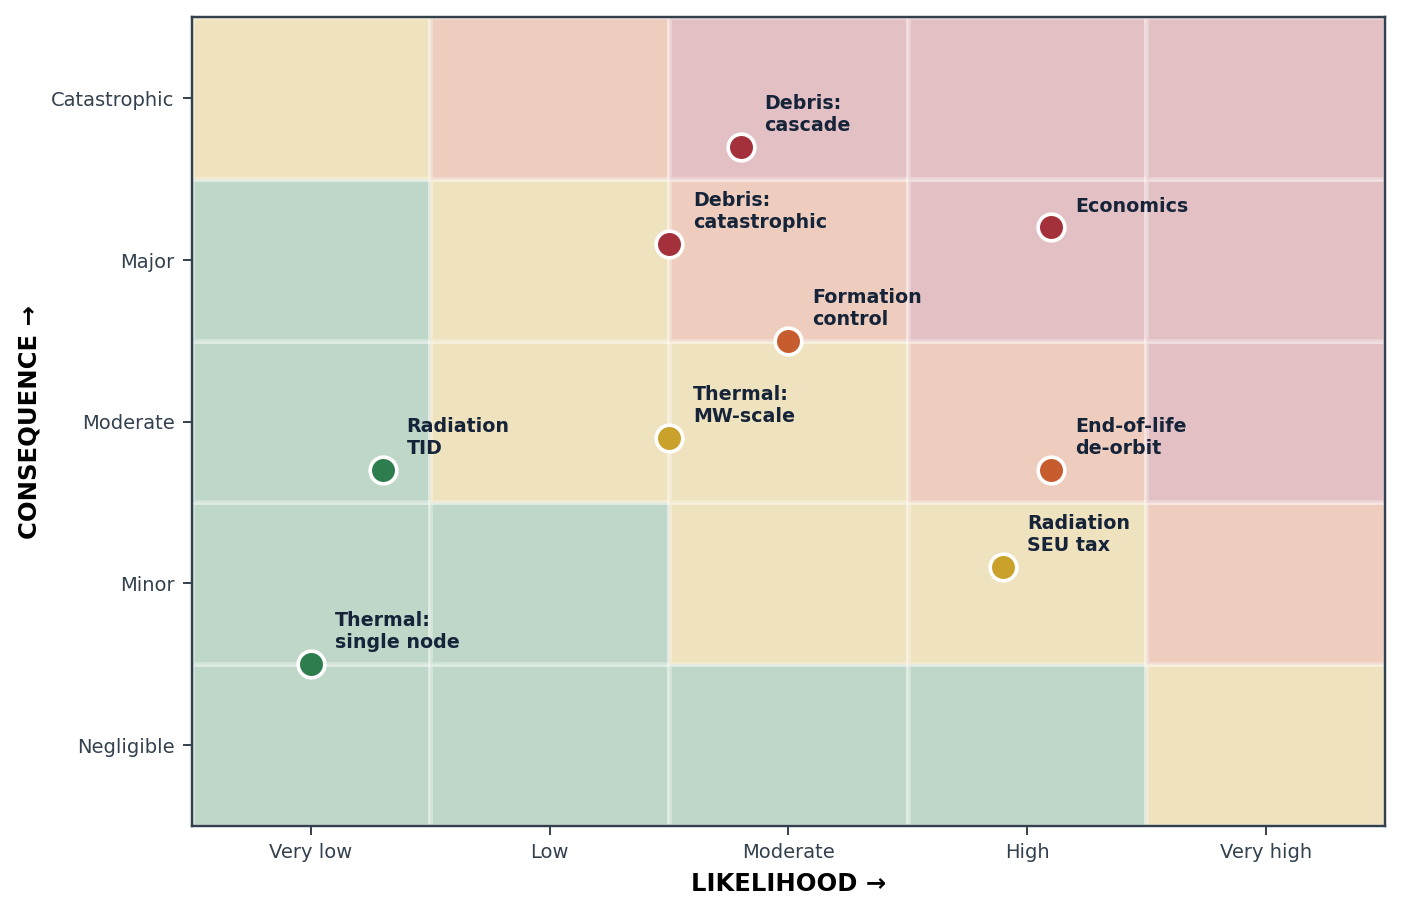
\includegraphics[keepaspectratio,alt={Fig. 25.1, Systems-level risk matrix: cooling is solved; debris, disposal, and economics are the open items.}]{figures/fig7_risk_matrix.png}}
\caption{Fig. 25.1, Systems-level risk matrix: cooling is solved;
debris, disposal, and economics are the open items.}
\end{figure}

\begin{center}\rule{0.5\linewidth}{0.5pt}\end{center}

\begin{center}\rule{0.5\linewidth}{0.5pt}\end{center}

\textbf{The disposal constraint and the propulsion it mandates.} The
chapter concludes that the 650-km orbit cannot meet the five-year
post-mission disposal rule passively, so propulsion is required. To see
why a controlled de-orbit burn is the natural remedy, begin from the
impulse needed to lower perigee into the dense atmosphere. For a
near-circular orbit of radius \(r\) about a body of gravitational
parameter \(\mu\), the circular speed follows from balancing gravity
against the centripetal requirement,

\begin{equation}
\frac{\mu}{r^{2}} = \frac{v_c^{2}}{r} \quad\Longrightarrow\quad v_c = \sqrt{\frac{\mu}{r}}. \tag{25.1}
\end{equation}

A single tangential retro-burn places the spacecraft on a transfer
ellipse whose apogee is the present radius \(r_a = R_\oplus + h\) and
whose perigee \(r_p\) is chosen low enough that drag completes the
decay. From the vis-viva relation,
\(v^{2} = \mu\!\left(2/r - 1/a\right)\) with semi-major axis
\(a = (r_a + r_p)/2\), the speed required at apogee is

\begin{equation}
v_a = \sqrt{\mu\!\left(\frac{2}{r_a} - \frac{2}{r_a + r_p}\right)}, \tag{25.2}
\end{equation}

so the de-orbit impulse is the deficit between the circular speed and
this transfer speed,

\begin{equation}
\Delta v_{\mathrm{deorbit}} = v_c - v_a = \sqrt{\frac{\mu}{r_a}} - \sqrt{\mu\!\left(\frac{2}{r_a} - \frac{2}{r_a + r_p}\right)}. \tag{25.3}
\end{equation}

The propellant mass to deliver this impulse is then set by the rocket
equation, with \(m_0\) the wet mass, \(m_f\) the dry mass, and
\(I_{sp}\) the specific impulse,

\begin{equation}
\frac{m_p}{m_0} = 1 - \exp\!\left(-\frac{\Delta v_{\mathrm{deorbit}}}{I_{sp}\, g_0}\right). \tag{25.4}
\end{equation}

\textbf{Worked example.} Take
\(\mu = 3.986\times10^{5}\ \mathrm{km^{3}/s^{2}}\),
\(R_\oplus = 6378\ \mathrm{km}\), and the chapter's
\(h = 650\ \mathrm{km}\), so \(r_a = 7028\ \mathrm{km}\) and
\(v_c = \sqrt{\mu/r_a} \approx 7.53\ \mathrm{km/s}\). Targeting a
perigee at \(r_p = R_\oplus + 100\ \mathrm{km} = 6478\ \mathrm{km}\)
gives \(a = 6753\ \mathrm{km}\) and \(v_a \approx 7.38\ \mathrm{km/s}\),
hence \(\Delta v_{\mathrm{deorbit}} \approx 0.15\ \mathrm{km/s}\). With
\(I_{sp} \approx 220\ \mathrm{s}\), equation (25.4) yields
\(m_p/m_0 \approx 1 - \exp(-150/2158) \approx 0.067\), roughly seven
percent of wet mass committed to disposal.

\textbf{Design implication.} A controlled de-orbit from the 650-km orbit
costs only a small velocity increment and a single-digit propellant
fraction, so the disposal risk is not one of feasibility but of
mandating, sizing, and reserving that propulsion within the demonstrator
from the outset rather than treating it as optional.

\part{DETAILED RESULTS, DATA, AND WORKED
COMPUTATIONS}\label{detailed-results-data-and-worked-computations}

\chapter{26. A Worked End-to-End
Computation}\label{a-worked-end-to-end-computation}

\begin{quote}
\emph{Abstract.} This chapter carries a single design point end to end,
from orbit through thermal, link, disposal, and compute, so the chain
from principle to number can be followed in one place.
\end{quote}

To make the integrated model concrete, this chapter walks through the
reference design point exactly as the code computes it, carrying the
numbers at each step. The inputs are four TPU-class accelerators at an
estimated 200 W each, a 650-km dawn-dusk orbit, a radiator operating
point of 45 C, 10 mm of aluminium shielding, a model-FLOPs utilization
of 0.30, error-correcting memory with checkpointing, moderate solar
activity, and a launch price of 300 dollars per kilogram.

The compute load is four times 200, or 800 W. The power budget adds 150
W of avionics, 80 W of attitude control, 50 W of communications, 20 W of
thermal control, and a fifteen-percent contingency, giving a total
electrical demand of 1,265 W and an electrical power-usage effectiveness
of 1.58 (Table T10). That total sizes a solar array of about five square
meters and a small dawn-dusk battery. The thermal load, compute plus
avionics plus parasitic, sizes a modest radiator by equation (10.3). The
radiation dose behind 10 mm of aluminium is about 1.05 krad(Si) over
five years, comfortably within the memory tolerance (Table T4). The
structural mass is taken as a fifth of the supported mass, and the
geometry yields an inertia of a few hundred kilogram-meters squared,
from which the gravity-gradient torque is of order one ten-thousandth of
a newton-meter. Summing all subsystems gives a dry mass near 220 kg
(Table T9), from which the drag area sets a ballistic coefficient that
feeds a natural lifetime of roughly twelve to twenty-two years depending
on solar activity, failing the five-year rule and mandating the 132 m/s
de-orbit burn of Table T7. The coupled thermal-throttle simulation
returns the delivered useful compute (about two-thirds of a petaflop for
this low-power, lightly throttled case), the ground-link model returns
tens of terabytes per day of downlink at ninety-six-percent
availability, and the finance model returns a levelized cost of roughly
one hundred dollars per useful petaflop-hour (Table T11). Aggregating
over the eighty-one-satellite cluster gives the fleet totals of Table
T12. Every one of these numbers is produced by the open code and is
reproduced by the validation suite.

\textbf{From compute load to electrical demand.} The chapter assembles
the bus power by summing the accelerator draw with the fixed subsystem
allocations and then applying a contingency factor. Writing
\(P_{\text{IT}}\) for the compute load and \(\{P_i\}\) for the avionics,
attitude-control, communications, and thermal-control allocations, the
total electrical demand is

\begin{equation}
P_{\text{elec}} = (1+m)\left(P_{\text{IT}} + \sum_i P_i\right), \tag{26.1}
\end{equation}

where \(m\) is the contingency margin. With
\(P_{\text{IT}} = 4 \times 200 = 800\) W, the subsystem sum
\(150 + 80 + 50 + 20 = 300\) W, and \(m = 0.15\), equation (26.1) gives
\(P_{\text{elec}} = 1.15 \times 1100 = 1{,}265\) W, the figure carried
in the text. The electrical power-usage effectiveness follows directly
as the ratio of total demand to compute draw,

\begin{equation}
\mathrm{PUE}_{\text{elec}} = \frac{P_{\text{elec}}}{P_{\text{IT}}} = \frac{1{,}265}{800} \approx 1.58, \tag{26.2}
\end{equation}

which reproduces the tabulated value and shows that the non-compute
overhead inflates the array and battery sizing by very nearly sixty
percent above the bare accelerator load.

\textbf{Lifetime, ballistic coefficient, and the disposal trigger.} The
natural orbital lifetime scales inversely with the ballistic
coefficient, so the dry-mass and drag-area estimates feed the disposal
decision. Defining the ballistic coefficient in the usual form,

\begin{equation}
\beta = \frac{m_{\text{dry}}}{C_D A}, \tag{26.3}
\end{equation}

a larger \(\beta\) means a denser, more compact body that lingers longer
at altitude. The de-orbit requirement is then governed by a simple
inequality between the natural lifetime \(T_{\text{nat}}(\beta)\) and
the regulatory limit \(T_{\text{rule}}\),

\begin{equation}
T_{\text{nat}}(\beta) > T_{\text{rule}} \;\Longrightarrow\; \text{active disposal required}. \tag{26.4}
\end{equation}

For the reference point \(T_{\text{nat}}\) falls in the
twelve-to-twenty-two-year band while \(T_{\text{rule}} = 5\) yr, so the
inequality holds and the active de-orbit burn of Table T7 is mandated;
the impulsive velocity increment of that burn is set by the
perigee-lowering maneuver and amounts to the 132 m/s already quoted.

\textbf{Levelized cost as a normalized figure of merit.} The finance
result is most useful when read as compute per unit cost. Writing
\(C_{\text{life}}\) for the lifecycle cost, \(Q\) for the delivered
useful compute rate, and \(T_{\text{op}}\) for the operating horizon,

\begin{equation}
\mathrm{LCC} = \frac{C_{\text{life}}}{Q \, T_{\text{op}}}, \tag{26.5}
\end{equation}

so the roughly one hundred dollars per useful petaflop-hour of Table T11
places the dominant leverage on \(Q\), the throttled compute, rather
than on launch price alone. Design implication: because
\(\mathrm{PUE}_{\text{elec}}\) and the throttled \(Q\) enter the cost
through (26.2) and (26.5), reducing parasitic overhead and thermal
throttling improves the economics more than equivalent reductions in
launch price, while the lifetime inequality (26.4) fixes disposal mass
and propellant before any of that economics is realized.

\chapter{27. Detailed Results Tables}\label{detailed-results-tables}

\begin{quote}
\emph{Abstract.} This chapter tabulates the detailed numerical results
that support the figures and conclusions of the preceding parts.
\end{quote}

The following tables report the model output across the relevant input
ranges. They are generated directly by the model
(\passthrough{\lstinline!report/gen\_tables.py!}) so that every value is
consistent with the equations of Parts II and III.

\textbf{Table T1, Orbital parameters versus altitude.} Speed, period,
critical beta angle, and natural lifetime. Note how steeply lifetime
rises with altitude, and that 650 km already fails the five-year rule at
moderate solar activity.

{\def\LTcaptype{none} % do not increment counter
\begin{longtable}[]{@{}
  >{\raggedright\arraybackslash}p{(\linewidth - 8\tabcolsep) * \real{0.2000}}
  >{\raggedright\arraybackslash}p{(\linewidth - 8\tabcolsep) * \real{0.2000}}
  >{\raggedright\arraybackslash}p{(\linewidth - 8\tabcolsep) * \real{0.2000}}
  >{\raggedright\arraybackslash}p{(\linewidth - 8\tabcolsep) * \real{0.2000}}
  >{\raggedright\arraybackslash}p{(\linewidth - 8\tabcolsep) * \real{0.2000}}@{}}
\toprule\noalign{}
\begin{minipage}[b]{\linewidth}\raggedright
Alt (km)
\end{minipage} & \begin{minipage}[b]{\linewidth}\raggedright
v (km/s)
\end{minipage} & \begin{minipage}[b]{\linewidth}\raggedright
Period (min)
\end{minipage} & \begin{minipage}[b]{\linewidth}\raggedright
β* (deg)
\end{minipage} & \begin{minipage}[b]{\linewidth}\raggedright
Lifetime, moderate (yr)
\end{minipage} \\
\midrule\noalign{}
\endhead
\bottomrule\noalign{}
\endlastfoot
400 & 7.67 & 92.4 & 70.2 & 5 \\
500 & 7.62 & 94.5 & 68.0 & 7 \\
600 & 7.56 & 96.5 & 66.1 & 13 \\
650 & 7.53 & 97.6 & 65.2 & 20 \\
700 & 7.51 & 98.6 & 64.3 & 32 \\
800 & 7.46 & 100.7 & 62.7 & 97 \\
1000 & 7.35 & 105.0 & 59.8 & 309 \\
\end{longtable}
}

\textbf{Table T2, Radiator area (m²) versus heat load and operating
temperature} (double-sided, ε = 0.90, 12 \% parasitic). The linearity in
load and the benefit of running hot are both visible.

{\def\LTcaptype{none} % do not increment counter
\begin{longtable}[]{@{}llll@{}}
\toprule\noalign{}
Heat load & 20 C & 40 C & 60 C \\
\midrule\noalign{}
\endhead
\bottomrule\noalign{}
\endlastfoot
1 kW & 2 & 1 & 1 \\
10 kW & 15 & 12 & 9 \\
100 kW & 151 & 116 & 90 \\
1 MW & 1,508 & 1,158 & 904 \\
\end{longtable}
}

\textbf{Table T3, Chip-interface temperature rise and passive
feasibility} (R\_th = 0.30 K/W). The interface wall is stark: every
GPU-class part exceeds the entire 125 C budget across the chain alone.

{\def\LTcaptype{none} % do not increment counter
\begin{longtable}[]{@{}llll@{}}
\toprule\noalign{}
Chip & TDP (W) & Interface ΔT (C) & Passive feasible (\textless125)? \\
\midrule\noalign{}
\endhead
\bottomrule\noalign{}
\endlastfoot
TPU v6e & 200 & 60 & yes \\
TPU & 300 & 90 & yes \\
H100 & 700 & 210 & NO \\
B200 & 1000 & 300 & NO \\
GB200 & 1200 & 360 & NO \\
\end{longtable}
}

\textbf{Table T4, Cumulative total ionizing dose, rad(Si), versus
aluminium shielding.} The 10-mm, five-year value of \textasciitilde1
krad sits comfortably below the 2-krad first-irregularity threshold.

{\def\LTcaptype{none} % do not increment counter
\begin{longtable}[]{@{}lll@{}}
\toprule\noalign{}
Al (mm) & 5-yr (rad) & 10-yr (rad) \\
\midrule\noalign{}
\endhead
\bottomrule\noalign{}
\endlastfoot
1 & 81,169 & 162,339 \\
3 & 25,479 & 50,959 \\
5 & 8,307 & 16,613 \\
10 & 1,054 & 2,109 \\
15 & 671 & 1,343 \\
20 & 651 & 1,302 \\
\end{longtable}
}

\textbf{Table T5, Catastrophic (\textgreater1 cm) debris probability
(\%) for the 81-satellite cluster.} The low/mid/high columns span the
ORDEM/MASTER flux band.

{\def\LTcaptype{none} % do not increment counter
\begin{longtable}[]{@{}llll@{}}
\toprule\noalign{}
Years & low flux & mid & high \\
\midrule\noalign{}
\endhead
\bottomrule\noalign{}
\endlastfoot
1 & 1.2 & 3.6 & 11.4 \\
2 & 2.4 & 7.0 & 21.6 \\
3 & 3.6 & 10.4 & 30.5 \\
5 & 5.9 & 16.7 & 45.5 \\
7 & 8.2 & 22.5 & 57.3 \\
10 & 11.4 & 30.5 & 70.3 \\
\end{longtable}
}

\textbf{Table T6, In-cluster cascade neighbor-hit probability (\%)
versus formation spacing.} The inverse-square fall-off is the formation
paradox quantified.

{\def\LTcaptype{none} % do not increment counter
\begin{longtable}[]{@{}ll@{}}
\toprule\noalign{}
Spacing (m) & P\_hit (\%) \\
\midrule\noalign{}
\endhead
\bottomrule\noalign{}
\endlastfoot
100 & 18.1 \\
150 & 8.5 \\
200 & 4.9 \\
300 & 2.2 \\
500 & 0.8 \\
1000 & 0.2 \\
\end{longtable}
}

\textbf{Table T7, Per-satellite Δv budget and propellant.} De-orbit
dominates; electric propulsion is dramatically lighter.

{\def\LTcaptype{none} % do not increment counter
\begin{longtable}[]{@{}ll@{}}
\toprule\noalign{}
Δv component & Value (m/s) \\
\midrule\noalign{}
\endhead
\bottomrule\noalign{}
\endlastfoot
Drag make-up & 14.7 \\
Formation keeping & 8.0 \\
Collision avoidance & 5.0 \\
Controlled de-orbit & 131.6 \\
Margin (20 \%) & 31.9 \\
\textbf{Total} & \textbf{191.2} \\
\end{longtable}
}

{\def\LTcaptype{none} % do not increment counter
\begin{longtable}[]{@{}lll@{}}
\toprule\noalign{}
Propulsion & Isp (s) & Propellant for total Δv (kg) \\
\midrule\noalign{}
\endhead
\bottomrule\noalign{}
\endlastfoot
Cold gas & 70 & 120 \\
Hydrazine & 220 & 35 \\
Electric & 1500 & 5 \\
\end{longtable}
}

\textbf{Table T8, Optical link budget versus range} (D = 0.1 m, λ = 1.55
µm). The +20 dB per decade of range, against a fixed \textasciitilde106
dB telescope gain, is why the cluster must be tight.

{\def\LTcaptype{none} % do not increment counter
\begin{longtable}[]{@{}lll@{}}
\toprule\noalign{}
Range & Telescope gain (dB) & Free-space loss (dB) \\
\midrule\noalign{}
\endhead
\bottomrule\noalign{}
\endlastfoot
150 m & 106 & 182 \\
1 km & 106 & 198 \\
100 km & 106 & 238 \\
1000 km & 106 & 258 \\
10000 km & 106 & 278 \\
\end{longtable}
}

\textbf{Table T9, Reference satellite mass budget} (four-chip bus,
closed by the integrated model).

{\def\LTcaptype{none} % do not increment counter
\begin{longtable}[]{@{}ll@{}}
\toprule\noalign{}
Subsystem & Mass (kg) \\
\midrule\noalign{}
\endhead
\bottomrule\noalign{}
\endlastfoot
Shielding & 54 \\
Avionics & 45 \\
ADCS & 30 \\
Harness & 28 \\
Structure & 27 \\
Power & 18 \\
Propulsion & 13 \\
Payload (chips) & 12 \\
Thermal & 6 \\
\textbf{Dry total} & \textbf{220} \\
Launch mass & 233 \\
\end{longtable}
}

\textbf{Table T10, Reference power budget.} Non-compute overhead
dominates a small bus, giving an electrical PUE near 1.6; efficiency
improves only at many-chip scale.

{\def\LTcaptype{none} % do not increment counter
\begin{longtable}[]{@{}ll@{}}
\toprule\noalign{}
Consumer & Power (W) \\
\midrule\noalign{}
\endhead
\bottomrule\noalign{}
\endlastfoot
Compute & 800 \\
Avionics & 150 \\
ADCS & 80 \\
Communications & 50 \\
Thermal control & 20 \\
Contingency & 165 \\
\textbf{Total} & \textbf{1,265} \\
Electrical PUE & 1.58 \\
\end{longtable}
}

\textbf{Table T11, Reference design-point summary} (all model outputs).

{\def\LTcaptype{none} % do not increment counter
\begin{longtable}[]{@{}ll@{}}
\toprule\noalign{}
Quantity & Value \\
\midrule\noalign{}
\endhead
\bottomrule\noalign{}
\endlastfoot
Compute power (W) & 800 \\
Total power (W) & 1,265 \\
Effective PUE & 1.84 \\
Radiator area (m²) & 1.1 \\
5-yr dose behind 10 mm (rad) & 1,054 \\
Dose margin (vs 2 krad) & 1.9× \\
Natural lifetime (yr) & 11.5 \\
Debris P (5 yr) & 0.17 \\
Delivered (PFLOPS) & 0.67 \\
Throttle loss & 14 \% \\
Ground downlink (TB/day) & 26.9 \\
LCOE (USD/PFLOP-hr) & 108 \\
\end{longtable}
}

\textbf{Table T12, Constellation summary (81 satellites).}

{\def\LTcaptype{none} % do not increment counter
\begin{longtable}[]{@{}ll@{}}
\toprule\noalign{}
Quantity & Value \\
\midrule\noalign{}
\endhead
\bottomrule\noalign{}
\endlastfoot
Fleet compute (PFLOPS) & 54.1 \\
Fleet power (MW) & 0.10 \\
CAPEX (USD) & 146,621,400 \\
10-yr TCO (USD) & 317,621,400 \\
Capacity availability & 0.89 \\
\end{longtable}
}

\chapter{28. Constellation Design and Relative
Dynamics}\label{constellation-design-and-relative-dynamics}

\begin{quote}
\emph{Abstract.} This chapter treats the relative dynamics of the tight
formation, the Clohessy-Wiltshire relations and the station-keeping they
imply.
\end{quote}

\emph{Sources: the relative-motion (Clohessy-Wiltshire) equations and
constellation geometry follow Curtis {[}16{]} and Vallado {[}17{]}.}

The eighty-one satellites do not fly in a rigid grid; they orbit in a
loose formation governed by the linearized relative equations of motion.
About a circular reference orbit of mean motion \(n\), the
Clohessy-Wiltshire (Hill) equations describe a satellite's position
relative to a co-orbiting frame:

\begin{equation}
\ddot x - 3 n^2 x - 2 n \dot y = a_x, \quad \ddot y + 2 n \dot x = a_y, \quad \ddot z + n^2 z = a_z. \tag{28.1}
\end{equation}

In the absence of forcing, the radial (\(x\)) and cross-track (\(z\))
modes oscillate at the orbital rate \(n\), while the along-track (\(y\))
motion contains a secular term: any small difference in energy or any
differential acceleration produces a drift that grows linearly in time,
and a differential along-track acceleration produces a drift that grows
as \(t^2\). This is the central challenge of the formation: because the
satellites have slightly different ballistic coefficients, differential
atmospheric drag, itself varying by a factor of one hundred over the
solar cycle, drives an along-track drift of order
\(1.5\, \delta a_{\mathrm{drag}}\, t^2\). With a 150-m spacing budget,
even a small differential acceleration consumes the margin within hours
to days, so the formation requires active relative control. The
propellant for this control is modest (Table T7), but the sensing and
autonomy are not: maintaining a sub-200-m formation while remaining able
to perform a collision-avoidance maneuver, without that maneuver
endangering a neighbor, is an unsolved control problem at this density,
and it is the operational face of the formation paradox.

\textbf{Derivation of the relative equations of motion.} The Hill
(Clohessy-Wiltshire) relations of Eq. (28.1) follow from linearizing the
two-body acceleration about a circular reference orbit. Let the chief
move on a circular orbit of radius \(r_0\) with mean motion
\(n = \sqrt{\mu / r_0^3}\), and write the deputy position as \(r_0 + x\)
in the radial direction within a frame rotating at constant rate \(n\).
In a rotating frame the absolute acceleration carries Coriolis and
centrifugal terms,

\begin{equation}
\mathbf{a}_{\mathrm{abs}} = \ddot{\mathbf{r}}_{\mathrm{rel}} + 2\,\mathbf{n}\times\dot{\mathbf{r}}_{\mathrm{rel}} + \mathbf{n}\times(\mathbf{n}\times\mathbf{r}_{\mathrm{rel}}), \tag{28.2}
\end{equation}

with \(\mathbf{n} = n\,\hat{\mathbf{z}}\). Expanding the gravitational
acceleration to first order in the small displacement, the radial
gradient gives \(-\mu/(r_0+x)^2 \approx -n^2 r_0 + 2 n^2 x\), in which
the constant term is cancelled by the centrifugal term \(n^2 r_0\)
acting on the reference radius. Collecting the radial, along-track, and
cross-track components reproduces Eq. (28.1).

\textbf{Closed-form drift and the along-track secular term.} Setting the
forcing to zero and solving the homogeneous system shows that the
along-track coordinate accumulates a term proportional to the initial
radial offset and any energy mismatch. For a constant differential
acceleration \(\delta a\) applied along-track, integrating
\(\ddot y + 2 n \dot x = \delta a\) together with the radial equation
yields, after the bounded oscillatory parts are removed, the secular
growth

\begin{equation}
y_{\mathrm{sec}}(t) \approx \tfrac{3}{2}\,\delta a\, t^2, \tag{28.3}
\end{equation}

which is the origin of the \(1.5\,\delta a_{\mathrm{drag}}\, t^2\)
estimate quoted in the chapter. The drift therefore scales quadratically
in time and linearly in the differential acceleration.

\textbf{Worked estimate.} Take a representative differential drag
acceleration
\(\delta a_{\mathrm{drag}} = 1\times 10^{-7}\ \mathrm{m\,s^{-2}}\) and
ask when the along-track offset reaches the 150-m spacing budget.
Inverting Eq. (28.3),

\begin{equation}
t_{\mathrm{budget}} = \sqrt{\frac{2\,\Delta y_{\max}}{3\,\delta a_{\mathrm{drag}}}} = \sqrt{\frac{2(150)}{3(10^{-7})}}\ \mathrm{s} \approx 3.2\times 10^{4}\ \mathrm{s}, \tag{28.4}
\end{equation}

about nine hours, consistent with the chapter's statement that margin is
consumed within hours to days.

\textbf{Design implication.} Because uncorrected along-track error grows
as \(t^2\) while the control budget is fixed at the 150-m spacing, the
formation must close its relative-navigation and thrust loop on a
timescale well inside \(t_{\mathrm{budget}}\); this sets the required
cadence of differential drag estimation and of the autonomous
station-keeping maneuvers rather than the total propellant.

\chapter{29. Comparison with Terrestrial Data
Centers}\label{comparison-with-terrestrial-data-centers}

\begin{quote}
\emph{Abstract.} This chapter sets the orbital architecture against
terrestrial hyperscale data centers, dimension by dimension, to locate
where each genuinely differs.
\end{quote}

It is instructive to place the orbital architecture beside a terrestrial
hyperscale facility on the metrics that matter (Table T13). Orbit wins
decisively on cooling overhead and water, and it offers a continuous
solar resource and freedom from land and grid constraints. It loses
decisively on serviceability (no repair), on the cost and risk of
launch, on radiation-induced throughput loss, and on the debris and
disposal obligations that have no terrestrial analogue. The reading is
that the two are not substitutes today: orbit is competitive only for
workloads that genuinely value what it uniquely provides, and only once
launch economics enter the parity band of Chapter 22.

\textbf{Table T13, Orbital versus terrestrial data center
(qualitative).}

{\def\LTcaptype{none} % do not increment counter
\begin{longtable}[]{@{}
  >{\raggedright\arraybackslash}p{(\linewidth - 4\tabcolsep) * \real{0.3333}}
  >{\raggedright\arraybackslash}p{(\linewidth - 4\tabcolsep) * \real{0.3333}}
  >{\raggedright\arraybackslash}p{(\linewidth - 4\tabcolsep) * \real{0.3333}}@{}}
\toprule\noalign{}
\begin{minipage}[b]{\linewidth}\raggedright
Dimension
\end{minipage} & \begin{minipage}[b]{\linewidth}\raggedright
Terrestrial hyperscale
\end{minipage} & \begin{minipage}[b]{\linewidth}\raggedright
Orbital (this study)
\end{minipage} \\
\midrule\noalign{}
\endhead
\bottomrule\noalign{}
\endlastfoot
Cooling & chillers/water, PUE \textasciitilde1.1-1.6 & radiative to 2.7
K; no water \\
Water use & millions of liters/yr & none \\
Power & grid, intermittent renewables & continuous solar (dawn-dusk) \\
Land & large footprint & none \\
Serviceability & hot-swap, on-site repair & none (no repair) \\
Radiation & negligible & \textasciitilde10-20 \% throughput tax \\
Disposal & decommission in place & mandatory propulsive de-orbit \\
Debris risk & none & binding constraint \\
Launch / deployment & trucking & USD/kg launch, dominant early cost \\
Latency (long-haul) & fiber (n=1.47) & vacuum mesh wins beyond
\textasciitilde3,000 km \\
\end{longtable}
}

\begin{center}\rule{0.5\linewidth}{0.5pt}\end{center}

\textbf{Power usage effectiveness as the cooling-overhead metric.} The
terrestrial column of Table T13 quotes a power usage effectiveness, or
PUE, in the band 1.1 to 1.6. This single figure of merit is defined as
the ratio of total facility power drawn from the grid to the power that
actually reaches the computing hardware,

\begin{equation}
\mathrm{PUE} = \frac{P_{\mathrm{facility}}}{P_{\mathrm{IT}}} = \frac{P_{\mathrm{IT}} + P_{\mathrm{cool}} + P_{\mathrm{aux}}}{P_{\mathrm{IT}}} = 1 + \frac{P_{\mathrm{cool}} + P_{\mathrm{aux}}}{P_{\mathrm{IT}}}, \tag{29.1}
\end{equation}

where \(P_{\mathrm{cool}}\) is the power consumed by chillers, pumps,
and fans, and \(P_{\mathrm{aux}}\) collects lighting, power-conversion
losses, and other ancillaries. The fraction of delivered power that
performs computation is the reciprocal,
\(\eta_{\mathrm{infra}} = 1/\mathrm{PUE}\). For a terrestrial facility
at \(\mathrm{PUE} = 1.5\) this useful fraction is \(1/1.5 = 0.67\), so
one third of the purchased energy is spent moving heat rather than
computing. The orbital architecture rejects heat by passive radiation to
the 2.7 K sky, as derived in Chapter 10, so its dedicated cooling term
\(P_{\mathrm{cool}}\) collapses toward the pumping power of the internal
coolant loop alone; this is the precise sense in which orbit wins on
cooling overhead.

\textbf{Radiation throughput tax.} The 10 to 20 percent figure in the
radiation row is an effective availability reduction. If single-event
upsets and dose-driven derating remove a fraction \(\tau_r\) of useful
cycles, the delivered compute of equation (17.1) is scaled to

\begin{equation}
C_{\mathrm{eff}} = n\,P_{\mathrm{peak}}\,\mathrm{MFU}\,a_r\,(1 - \tau_r), \tag{29.2}
\end{equation}

so that the parity comparison must be made on \(C_{\mathrm{eff}}\), not
on nameplate capacity. With \(\tau_r\) in the stated range the orbital
cluster must over-provision hardware by a factor \(1/(1-\tau_r)\) to
match a terrestrial throughput target.

\textbf{Latency crossover.} The latency row asserts that a vacuum mesh
overtakes terrestrial fiber beyond roughly 3,000 km. Signal speed in
fiber is \(c/n\) with refractive index \(n = 1.47\), while a free-space
optical link propagates at \(c\). For a great-circle ground separation
\(L\) the one-way times are \(t_{\mathrm{fiber}} = nL/c\) and,
neglecting the modest path stretch to orbit,
\(t_{\mathrm{space}} \approx L/c\), so the vacuum advantage grows
linearly with distance,

\begin{equation}
\Delta t = t_{\mathrm{fiber}} - t_{\mathrm{space}} = \frac{(n-1)\,L}{c}. \tag{29.3}
\end{equation}

At \(L = 3{,}000\) km this gives
\(\Delta t = 0.47 \times 3{\times}10^{6}/(3{\times}10^{8}) \approx 4.7\)
ms of saved one-way latency before any orbital path penalty is charged.
The design implication is that orbit competes on latency only for
genuinely intercontinental traffic, and on cost only inside the
launch-parity band of Chapter 22; for regional workloads the terrestrial
facility remains the lower-risk choice.

\part{Appendices and Back Matter}\label{appendices-and-back-matter}

\chapter{References}\label{references}

\begin{enumerate}
\def\labelenumi{\arabic{enumi}.}
\tightlist
\item
  Agüera y Arcas et al.~(2025). \emph{Towards a future space-based,
  highly scalable AI infrastructure system design.} arXiv:2511.19468.
\item
  Google. \emph{Project Suncatcher.}
  blog.google/innovation-and-ai/technology/research/google-project-suncatcher/
\item
  Planet Labs. \emph{Platform for Project Suncatcher.} planet.com/pulse/
\item
  NVIDIA. \emph{Starcloud, H100 in orbit.}
  blogs.nvidia.com/blog/starcloud/
\item
  Axiom Space. \emph{Orbital Data Center nodes.} axiomspace.com
\item
  Liang et al.~(2022). \emph{Link Budget Analysis for Free-Space Optical
  Satellite Networks.} arXiv:2204.13177.
\item
  FCC. \emph{Five-Year Rule (FCC 22-74).} fcc.gov ; Federal Register
  2024-17093.
\item
  NASA. \emph{ORDEM 3.2 User Guide.} NTRS 20230014989.
\item
  ESA. \emph{MASTER / DRAMA debris tools.}
  esa.int/Space\_Safety/Space\_Debris/
\item
  SPENVIS. \emph{SHIELDOSE.} spenvis.oma.be
\item
  Picone et al.~(2002). \emph{NRLMSISE-00 empirical atmosphere model.}
  JGR, doi:10.1029/2002JA009430.
\item
  NVIDIA H100 / B200 / GB200 datasheets; Google Cloud TPU v6e
  documentation; Azur/Spectrolab solar-cell datasheets; NASA ISS Active
  Thermal Control System overview.
\item
  NASA Systems Engineering Handbook, NASA/SP-2016-6105.
\item
  AIAA S-120-2006, Mass Properties Control for Space Systems.
\item
  NASA Goddard Integrated Design Center, concurrent-design margin
  practice (NTRS 20120013284).
\item
  Curtis, H. D. \emph{Orbital Mechanics for Engineering Students}, 4th
  ed.~Butterworth-Heinemann, 2020.
\item
  Vallado, D. A. \emph{Fundamentals of Astrodynamics and Applications},
  4th ed.~Microcosm Press, 2013.
\item
  Wertz, J. R., Everett, D. F., Puschell, J. J. (eds.). \emph{Space
  Mission Engineering: The New SMAD.} Microcosm Press, 2011.
\item
  Larson, W. J., Wertz, J. R. (eds.). \emph{Space Mission Analysis and
  Design}, 3rd ed.~Microcosm/Kluwer, 1999.
\item
  Gilmore, D. G. (ed.). \emph{Spacecraft Thermal Control Handbook,
  Volume I: Fundamental Technologies}, 2nd ed.~The Aerospace Press,
  2002.
\item
  Incropera, F. P., DeWitt, D. P., Bergman, T. L., Lavine, A. S.
  \emph{Fundamentals of Heat and Mass Transfer}, 7th ed.~Wiley, 2011.
\item
  Tribble, A. C. \emph{The Space Environment: Implications for
  Spacecraft Design}, rev. ed.~Princeton University Press, 2003.
\item
  Pisacane, V. L. (ed.). \emph{The Space Environment and Its Effects on
  Space Systems}, 2nd ed.~AIAA Education Series, 2016.
\item
  Hastings, D., Garrett, H. \emph{Spacecraft-Environment Interactions.}
  Cambridge University Press, 1996.
\item
  Vette, J. I. \emph{The AE-8 Trapped Electron Model Environment}
  (NSSDC/WDC-A-R\&S 91-24); Sawyer, D. M., Vette, J. I. \emph{AP-8
  Trapped Proton Environment} (NSSDC/WDC-A-R\&S 76-06). NASA GSFC.
\item
  Ginet, G. P. et al.~\emph{AE9, AP9 and SPM: New Models for Specifying
  the Trapped Energetic Particle and Space Plasma Environment.} Space
  Science Reviews 179, 2013.
\item
  Seltzer, S. M. \emph{SHIELDOSE: A Computer Code for Space-Shielding
  Radiation Dose Calculations.} NBS Technical Note 1116, 1980.
\item
  Kessler, D. J., Cour-Palais, B. G. \emph{Collision Frequency of
  Artificial Satellites: The Creation of a Debris Belt.} Journal of
  Geophysical Research 83(A6), 1978.
\item
  Klinkrad, H. \emph{Space Debris: Models and Risk Analysis.}
  Springer-Praxis, 2006.
\item
  Hemmati, H. (ed.). \emph{Deep Space Optical Communications.} JPL
  Deep-Space Communications and Navigation Series, Wiley, 2006.
\item
  Sutton, G. P., Biblarz, O. \emph{Rocket Propulsion Elements}, 9th
  ed.~Wiley, 2017.
\item
  Wertz, J. R. (ed.). \emph{Spacecraft Attitude Determination and
  Control.} D. Reidel, 1978.
\item
  Sidi, M. J. \emph{Spacecraft Dynamics and Control: A Practical
  Engineering Approach.} Cambridge University Press, 1997.
\item
  ECSS. \emph{Space Engineering: Thermal Control General Requirements}
  (ECSS-E-ST-31C) and \emph{Space Environment} (ECSS-E-ST-10-04C).
  European Cooperation for Space Standardization.
\item
  O'Hanlon, M. et al.; SpaceX published launch-manifest and reusability
  data; FAA commercial-space launch records, for the launch-cadence and
  cost-trajectory inputs of Chapter 22.
\end{enumerate}

\chapter{Appendix A, Master List of Governing
Equations}\label{appendix-a-master-list-of-governing-equations}

{\def\LTcaptype{none} % do not increment counter
\begin{longtable}[]{@{}
  >{\raggedright\arraybackslash}p{(\linewidth - 4\tabcolsep) * \real{0.3333}}
  >{\raggedright\arraybackslash}p{(\linewidth - 4\tabcolsep) * \real{0.3333}}
  >{\raggedright\arraybackslash}p{(\linewidth - 4\tabcolsep) * \real{0.3333}}@{}}
\toprule\noalign{}
\begin{minipage}[b]{\linewidth}\raggedright
\#
\end{minipage} & \begin{minipage}[b]{\linewidth}\raggedright
Quantity
\end{minipage} & \begin{minipage}[b]{\linewidth}\raggedright
Equation
\end{minipage} \\
\midrule\noalign{}
\endhead
\bottomrule\noalign{}
\endlastfoot
4.1 & Circular speed & \(v = \sqrt{\mu/a}\) \\
4.2 & Period / mean motion & \(T = 2\pi\sqrt{a^3/\mu}\),
\(n=\sqrt{\mu/a^3}\) \\
4.3 & Specific energy & \(\mathcal{E} = -\mu/2a\) \\
5.2 & SSO inclination &
\(\cos i = -2\dot\Omega_{\mathrm{sun}} a^2/(3 n J_2 R_E^2)\) \\
6.1 & Critical beta & \(\beta^{*} = \arcsin(R_E/(R_E+h))\) \\
7.3 & Orbital decay & \(\dot a = -C_D (A/m)\,\rho\,\sqrt{\mu a}\) \\
8.1 & Dose-depth & \(\dot D(x) = D_0 e^{-x/\lambda} + D_\infty\) \\
9.1 & Debris risk & \(P = 1 - e^{-\Phi A N t}\) \\
10.2 & Stefan-Boltzmann & \(E_b = \sigma T^4\) \\
10.3 & Radiator area &
\(A_{\mathrm{rad}} = Q/[\varepsilon\sigma T^4 n_s(1-f_p)]\) \\
11.1 & Array power &
\(P = S_0 A\,\eta\,\kappa\,\eta_{\mathrm{path}}\) \\
12.1 & Panel frequency & \(f_1 = (\beta/2\pi)\sqrt{D/(\rho_A a^4)}\) \\
13.1 & Gravity-gradient torque &
\(\tau_{\mathrm{gg}} = \tfrac{3}{2}\, n^2\, \Delta I\, \sin 2\theta\) \\
14.1 & Telescope gain / FSPL & \(G=(\pi D/\lambda)^2\),
\(L_{\mathrm{fs}}=(4\pi R/\lambda)^2\) \\
15.1 & De-orbit Δv & \(\Delta v = v_{c1}(1-\sqrt{2 r_2/(r_1+r_2)})\) \\
15.2 & Propellant &
\(m_p = m_{\mathrm{dry}}(e^{\Delta v/I_{sp}g_0}-1)\) \\
16.1 & Reliability & \(R(t) = e^{-t/\mathrm{MTBF}}\) \\
16.2 & k-of-n &
\(R_{\mathrm{sys}}=\sum_{i=k}^n \binom{n}{i}p^i(1-p)^{n-i}\) \\
17.1 & Delivered compute & \(n P_{\mathrm{peak}}\,\mathrm{MFU}\,a_r\) \\
21.1 & LCOE &
\((\mathrm{CRF}\cdot\mathrm{CAPEX}+\mathrm{OPEX})/\text{useful PFLOP-hr}\) \\
\end{longtable}
}

\chapter{Appendix B, Nomenclature}\label{appendix-b-nomenclature}

See the Nomenclature table in the front matter; every symbol used in the
equations above is defined there with its units.

\chapter{Appendix C, Data Sources and
Confidence}\label{appendix-c-data-sources-and-confidence}

Every model input is tabulated with its value, source, and a confidence
flag (official / model / estimate) in the companion repository's
\passthrough{\lstinline!systems-model/docs/SOURCES.md!}. The dominant
caveats are repeated here: the chip power is undisclosed and treated as
an estimate; the solar-cycle density swing of roughly one hundred is the
largest physical uncertainty and is shown as a band; and the
1-mm-to-1-cm debris flux is the least model-validated quantity.

\chapter{Appendix D, Reproduction and
Code}\label{appendix-d-reproduction-and-code}

The entire analysis is open. From the repository,

\begin{lstlisting}
git clone https://github.com/Samarjithbiswas/space-based-ai-datacenter
cd space-based-ai-datacenter && pip install numpy matplotlib pytest
python reproduce_all.py        # both models, all figures, equation images
python report/predictions.py   # the launch-cost-parity Monte-Carlo
\end{lstlisting}

The systems model comprises seventeen subsystem modules plus an
integration layer and a Monte-Carlo engine, validated by 108 automated
tests. Each module's docstring states its governing equation; the
mathematical derivations in this volume are the authoritative reference.
Independent reproduction, extension, and correction are welcome through
the repository's issues and pull requests.

For completeness, the core physics functions are listed below; each is a
direct, pure implementation of the corresponding equation in this
volume.

\textbf{Orbital decay, Eq. (7.3).}

\begin{lstlisting}[language=Python]
def lifetime_years(alt_km, area_to_mass, scenario="mod", cd=2.2):
    a, t, yr, dt = R_E + alt_km*1e3, 0.0, 3.15576e7, 3600*6
    while a > R_E + 120e3 and t < 2000*yr:
        h = (a - R_E)/1e3
        a += -cd*area_to_mass*density(h, scenario)*np.sqrt(MU*a)*dt; t += dt
        dt = 3600*48 if (a-R_E) > 500e3 else (3600*12 if (a-R_E) > 300e3 else 3600*2)
    return t/yr
\end{lstlisting}

\textbf{Radiator sizing, Eq. (10.3).}

\begin{lstlisting}[language=Python]
def radiator_area(heat_W, temp_C, emissivity=0.90, sides=2, parasitic=0.12):
    T = temp_C + 273.15
    return heat_W / (emissivity * SIGMA * T**4 * sides * (1 - parasitic))
\end{lstlisting}

\textbf{Debris collision probability, Eq. (9.1).}

\begin{lstlisting}[language=Python]
def collision_probability(cross_section_m2, n_sats, years, size="1cm", band="mid"):
    flux = debris_flux(size, band)
    return 1 - np.exp(-flux * cross_section_m2 * n_sats * years)
\end{lstlisting}

\textbf{Controlled de-orbit Δv, Eq. (15.1).}

\begin{lstlisting}[language=Python]
def deorbit_delta_v(alt_km, perigee_km=180.0):
    r1, r2 = R_E + alt_km*1e3, R_E + perigee_km*1e3
    v1 = np.sqrt(MU / r1)
    return v1 * (1 - np.sqrt(2*r2 / (r1 + r2)))
\end{lstlisting}

\textbf{Coupled thermal-throttle workload (excerpt), Chapter 17.}

\begin{lstlisting}[language=Python]
def throttle_factor(T_j, T_throttle=110.0, T_max=125.0):
    return float(np.clip((T_max - T_j) / (T_max - T_throttle), 0.0, 1.0))
# in the time loop: T_j = T_rad_C + P_full*r_th; u_eff = u_cmd * throttle_factor(T_j)
# C dT/dt = Q_in - eps*sigma*A_eff*T^4   (forward Euler over one orbit)
\end{lstlisting}

\textbf{Levelized cost of compute, Eq. (21.1).}

\begin{lstlisting}[language=Python]
def lcoe_per_pflop_hr(capex, opex_yr, delivered_pflops, rate=0.10, life=5, util=0.8):
    crf = rate*(1+rate)**life / ((1+rate)**life - 1)
    return (crf*capex + opex_yr) / (delivered_pflops * 8766.0 * util)
\end{lstlisting}

\chapter{Appendix E, Extended
Derivations}\label{appendix-e-extended-derivations}

This appendix gives the full step-by-step derivations of the results
quoted in compressed form in the main text, so that the volume is
mathematically self-contained.

\section{E.1 Stefan-Boltzmann law from Planck's
law}\label{e.1-stefan-boltzmann-law-from-plancks-law}

Starting from the spectral radiance (10.1), the hemispherical emissive
power is the integral of the radiance over the emitting hemisphere and
all wavelengths. The angular integral over the hemisphere, weighted by
the projection factor \(\cos\theta\), is

\[\int_{\mathrm{hemi}} \cos\theta\, d\Omega = \int_0^{2\pi}\!\!\int_0^{\pi/2} \cos\theta\,\sin\theta\, d\theta\, d\phi = 2\pi\cdot\tfrac{1}{2} = \pi.\]

Hence \(E_b(T) = \pi\int_0^\infty B(\lambda, T)\, d\lambda\).
Substituting Planck's law and changing variables to
\(u = h_P c/(\lambda k_B T)\), so that \(\lambda = h_P c/(u k_B T)\) and
\(d\lambda = -h_P c/(u^2 k_B T)\, du\), the wavelength integral becomes

\[E_b(T) = \frac{2\pi k_B^4 T^4}{h_P^3 c^2}\int_0^\infty \frac{u^3}{e^u - 1}\, du.\]

The remaining integral is a standard result,
\(\int_0^\infty u^3/(e^u-1)\, du = \pi^4/15\), giving

\[E_b(T) = \frac{2\pi^5 k_B^4}{15\, h_P^3 c^2}\, T^4 \equiv \sigma T^4,\]

which both proves the fourth-power law and yields the Stefan-Boltzmann
constant in terms of fundamental constants. This is the foundation of
every radiator result in Chapter 10.

\section{E.2 The Poisson impact model from the binomial
limit}\label{e.2-the-poisson-impact-model-from-the-binomial-limit}

Divide the mission duration \(t\) into \(n\) equal intervals
\(\Delta t = t/n\). In each interval the probability of one impact is
\(p = \Phi A \Delta t\) (flux times cross-section times time), and
impacts in different intervals are independent. The number of impacts
\(K\) is therefore binomial, \(P(K=k) = \binom{n}{k} p^k (1-p)^{n-k}\).
Hold the expected count \(\Lambda = n p = \Phi A t\) fixed and let
\(n\to\infty\) (so \(p\to 0\)). Then
\(\binom{n}{k} p^k \to \Lambda^k/k!\) and
\((1-p)^{n-k} \to e^{-\Lambda}\), so

\[P(K=k) = \frac{\Lambda^k e^{-\Lambda}}{k!}.\]

The probability of at least one impact is
\(P(K\ge 1) = 1 - P(K=0) = 1 - e^{-\Lambda}\). For \(N\) independent
satellites the expected count scales to \(\Lambda = \Phi A N t\), giving
equation (9.1). This is exact in the limit of many small independent
intervals, the appropriate regime for rare debris impacts.

\section{E.3 The Hohmann de-orbit impulse from
vis-viva}\label{e.3-the-hohmann-de-orbit-impulse-from-vis-viva}

The vis-viva relation for any Keplerian orbit is
\(v^2 = \mu(2/r - 1/a)\), obtained from conservation of the specific
energy \(\mathcal{E} = v^2/2 - \mu/r = -\mu/2a\). Consider a transfer
ellipse whose apogee touches the circular orbit at \(r_1\) and whose
perigee is lowered to \(r_2\); its semi-major axis is
\(a_t = (r_1 + r_2)/2\). The speed required at the apogee of this
transfer is

\[v_{\mathrm{apo}} = \sqrt{\mu\left(\frac{2}{r_1} - \frac{1}{a_t}\right)}
= \sqrt{\mu\left(\frac{2}{r_1} - \frac{2}{r_1 + r_2}\right)}
= \sqrt{\frac{\mu}{r_1}}\sqrt{\frac{2 r_2}{r_1 + r_2}}.\]

The satellite is initially on the circular orbit at speed
\(v_{c1} = \sqrt{\mu/r_1}\), so the retrograde impulse needed is the
difference,

\[\Delta v_{\mathrm{deorbit}} = v_{c1} - v_{\mathrm{apo}} = v_{c1}\left(1 - \sqrt{\frac{2 r_2}{r_1 + r_2}}\right),\]

which is equation (15.1). Lowering the perigee into the dense atmosphere
(here to 180 km) guarantees re-entry within one or two orbits,
satisfying the disposal requirement.

\section{E.4 The Clohessy-Wiltshire relative
equations}\label{e.4-the-clohessy-wiltshire-relative-equations}

Let a chief satellite move on a circular orbit of radius \(r_0\) and
mean motion \(n = \sqrt{\mu/r_0^3}\), and let a deputy be displaced by a
small vector \((x, y, z)\) in the rotating Hill frame (radial,
along-track, cross-track). Writing Newton's equation for the deputy,
expanding the gravity gradient to first order in the small displacement,
and accounting for the frame rotation (Coriolis and centrifugal terms)
yields the linearized system

\[\ddot x - 2 n \dot y - 3 n^2 x = a_x, \quad \ddot y + 2 n \dot x = a_y, \quad \ddot z + n^2 z = a_z.\]

The cross-track equation is a simple harmonic oscillator at frequency
\(n\). The in-plane equations couple radial and along-track motion;
their unforced solution contains bounded oscillations at \(n\) plus a
secular along-track drift proportional to any initial energy mismatch.
Crucially, a constant differential along-track acceleration \(a_y\)
(such as differential drag) integrates twice into an along-track
displacement that grows as \(\tfrac{1}{2} a_y t^2\) to leading order,
augmented by the Coriolis coupling to a coefficient of order
\(\tfrac{3}{2}\), which is the quadratic-in-time drift discussed in
Chapter 28 and the reason the formation needs active relative control.

\section{E.5 The rocket equation}\label{e.5-the-rocket-equation}

A rocket of instantaneous mass \(m\) expelling propellant at exhaust
speed \(v_e\) relative to the vehicle changes its momentum according to
\(m\, dv = -v_e\, dm\) (the mass decreases as propellant is ejected,
hence the minus sign). Separating variables and integrating from the
initial mass \(m_0\) to the final (dry) mass \(m_f\),

\[\int_0^{\Delta v} dv = -v_e \int_{m_0}^{m_f} \frac{dm}{m} \;\Longrightarrow\; \Delta v = v_e \ln\frac{m_0}{m_f}.\]

With \(v_e = I_{sp} g_0\) and \(m_f = m_{\mathrm{dry}}\), the propellant
mass \(m_p = m_0 - m_f\) follows by inverting:

\[m_p = m_{\mathrm{dry}}\left(e^{\Delta v/(I_{sp} g_0)} - 1\right),\]

which is equation (15.2). The exponential dependence is why a high
specific impulse (electric propulsion) so dramatically reduces
propellant mass for a given Δv.

\section{E.6 k-of-n redundancy}\label{e.6-k-of-n-redundancy}

If \(n\) identical units each survive independently with probability
\(p\), the number that survive is binomial. The system requires at least
\(k\) survivors, so its reliability is the upper tail of the binomial
distribution,

\[R_{\mathrm{sys}} = \sum_{i=k}^{n} \binom{n}{i}\, p^i (1-p)^{n-i}.\]

Two special cases are familiar: a parallel (one-of-\(n\)) system has
\(R = 1 - (1-p)^n\), and a series (\(n\)-of-\(n\)) system has
\(R = p^n\). This expression sizes both the spare accelerators within a
satellite and the over-provisioned satellites within a cluster (Chapter
16).

\section{E.7 Newton-Raphson for the radiator
quartic}\label{e.7-newton-raphson-for-the-radiator-quartic}

To find the radiator temperature at fixed area, one solves
\(f(T) = Q - \varepsilon\sigma A T^4 = 0\). Newton's method linearizes
\(f\) about the current iterate:
\(f(T + \delta) \approx f(T) + f'(T)\delta\), set to zero gives
\(\delta = -f(T)/f'(T)\), hence

\[T_{k+1} = T_k - \frac{f(T_k)}{f'(T_k)} = T_k + \frac{Q - \varepsilon\sigma A T_k^4}{4\,\varepsilon\sigma A T_k^3}.\]

Because \(f\) is smooth and strictly decreasing for \(T>0\) (its
derivative \(-4\varepsilon\sigma A T^3\) never vanishes there), the
iteration converges quadratically from any reasonable start; in
practice, from \(T_0 = 300\) K it reaches a tolerance of \(0.01\) K in
two to four steps.

\section{E.8 The capital-recovery
factor}\label{e.8-the-capital-recovery-factor}

The capital-recovery factor converts a present capital sum \(C\) into an
equivalent stream of \(n\) equal annual payments \(X\) at discount rate
\(r\). The present value of the payment stream is a finite geometric
series,

\[C = \sum_{t=1}^{n} \frac{X}{(1+r)^t} = X\,\frac{1 - (1+r)^{-n}}{r}.\]

Solving for the annual payment per unit capital gives

\[\mathrm{CRF} = \frac{X}{C} = \frac{r(1+r)^n}{(1+r)^n - 1},\]

used in the levelized-cost-of-compute formula (21.1) to annualize the
satellite hardware and launch cost over its operational life.

\backmatter
% Back matter: About the Author. Injected by pandoc as include-after-body,
% so it sits after the body in the back-matter region.
\clearpage
\chapter*{About the Author}
\addcontentsline{toc}{chapter}{About the Author}

\noindent Samarjith Biswas, PhD, is a research scientist working at the intersection of computational
physics, engineering design, and machine-learning surrogates for physical systems. His work spans
wave physics, thermal and acoustic engineering, and the development of open, reproducible modeling
tools, several of which are published as open-access handbooks and browser-deployed design suites.

\vspace{8pt}
\noindent This book continues that practice: the analysis is paired with an open-source simulation
model, and every figure and load-bearing number is reproducible from the public repository. The
author's other open toolkits and reports are collected at \texttt{samarjithbiswas.com}.

\vspace{8pt}
\noindent Correspondence and corrections are welcome through the project repository,
\texttt{github.com/Samarjithbiswas/space-based-ai-datacenter}.

\end{document}
